%========================================================================================
%  Tesis de maestría — Predictibilidad de los precios mayoristas de alimentos en Colombia
%  Proyecto para Overleaf. Compilador: pdfLaTeX. Bibliografía: biblatex (backend bibtex).
%  Si la clase MastersDoctoralThesis.cls no está en el proyecto, se usa un diseño
%  equivalente (fallback_thesis.tex) para que el documento compile igual.
%========================================================================================
\IfFileExists{MastersDoctoralThesis.cls}{%
\documentclass[
11pt,
english, % Se mantiene como en la plantilla; los textos fijos se traducen más abajo
openany, % Sin páginas en blanco antes de cada capítulo (máximo 50 páginas)
singlespacing,
headsepline,
]{MastersDoctoralThesis}
\newcommand{\usandoplantilla}{}
}{%
\documentclass[11pt,a4paper,twoside,openany]{book}
% ---------------------------------------------------------------------------------------
% Diseño de respaldo: solo se usa si MastersDoctoralThesis.cls no está en el proyecto.
% Imita la apariencia de la plantilla Masters/Doctoral Thesis (Palatino, dos caras,
% títulos de capítulo del estilo book, encabezado con línea, páginas de resumen y
% agradecimientos centradas) para que el documento se vea igual sin la clase.
% ---------------------------------------------------------------------------------------
\usepackage[includehead]{geometry}
\usepackage{fancyhdr}
\usepackage[english,spanish,es-noshorthands,es-nodecimaldot,es-nolayout,es-tabla,es-nosectiondot]{babel}
\usepackage{setspace}
\usepackage{longtable}
\usepackage[hidelinks]{hyperref}

% ---- comandos de la plantilla
\newcommand{\thesistitle}[1]{\def\ttitle{#1}}
\newcommand{\supervisor}[1]{\def\supname{#1}}
\newcommand{\examiner}[1]{\def\examname{#1}}
\newcommand{\degree}[1]{\def\degreename{#1}}
\renewcommand{\author}[1]{\def\authorname{#1}}
\newcommand{\addresses}[1]{\def\addressname{#1}}
\newcommand{\subject}[1]{\def\subjectname{#1}}
\newcommand{\keywords}[1]{\def\keywordnames{#1}}
\newcommand{\university}[1]{\def\univname{#1}}
\newcommand{\department}[1]{\def\deptname{#1}}
\newcommand{\group}[1]{\def\groupname{#1}}
\newcommand{\faculty}[1]{\def\facname{#1}}
\newcommand{\HRule}{\rule{\linewidth}{.4mm}}
\newcommand{\addchaptertocentry}[1]{\addcontentsline{toc}{chapter}{#1}}

% ---- resumen y agradecimientos con el diseño centrado de la plantilla
\newcommand{\abstractname}{Resumen}
\newenvironment{abstract}{%
  \cleardoublepage\thispagestyle{plain}
  \begin{center}
  {\normalsize\scshape\univname\par}\bigskip
  {\huge\textit{\abstractname}\par}\bigskip
  {\normalsize\facname\par}{\normalsize\deptname\par}\bigskip
  {\normalsize\degreename\par}\bigskip
  {\normalsize\bfseries\ttitle\par}\medskip
  {\normalsize por \authorname\par}\bigskip
  \end{center}}{\vfil\null}
\newcommand{\acknowledgementname}{Agradecimientos}
\newenvironment{acknowledgements}{%
  \cleardoublepage\thispagestyle{plain}
  \begin{center}{\huge\textit{\acknowledgementname}\par}\end{center}\bigskip}{\vfil\null}
\newcommand{\abbrevname}{Lista de abreviaturas}
\newenvironment{abbreviations}[1]{\cleardoublepage\chapter*{\abbrevname}\begin{longtable}{#1}}{\end{longtable}}
\newcommand{\dedicatory}[1]{\cleardoublepage\thispagestyle{plain}\vspace*{.2\textheight}\begin{center}\itshape #1\end{center}}

% ---- encabezados (con línea bajo el encabezado, como la opción headsepline)
\fancypagestyle{thesis}{\fancyhf{}%
  \fancyhead[LE,RO]{\thepage}%
  \fancyhead[RE]{\itshape\nouppercase{\leftmark}}%
  \fancyhead[LO]{\itshape\nouppercase{\rightmark}}%
  \renewcommand{\headrulewidth}{0.4pt}}
\fancypagestyle{plain}{\fancyhf{}\fancyfoot[C]{\thepage}\renewcommand{\headrulewidth}{0pt}}

% ---- títulos de capítulo con el estilo de la plantilla, pero con menos espacio vertical
\makeatletter
\def\@makechapterhead#1{\vspace*{10\p@}{\parindent\z@\raggedright\normalfont
  \ifnum\c@secnumdepth>\m@ne\if@mainmatter\huge\bfseries\@chapapp\space\thechapter\par\nobreak\vskip 12\p@\fi\fi
  \interlinepenalty\@M\Huge\bfseries #1\par\nobreak\vskip 24\p@}}
\def\@makeschapterhead#1{\vspace*{10\p@}{\parindent\z@\raggedright\normalfont
  \interlinepenalty\@M\Huge\bfseries #1\par\nobreak\vskip 24\p@}}
\makeatother

}

\usepackage{array}
\usepackage{longtable}
\usepackage{adjustbox}
\usepackage{multirow}
\usepackage{caption}\captionsetup{font=small,skip=4pt}\setlength{\textfloatsep}{10pt plus 2pt minus 2pt}\setlength{\intextsep}{8pt plus 2pt minus 2pt}\setlength{\floatsep}{8pt plus 2pt minus 2pt}
\usepackage{amsmath}
\usepackage{amssymb}
\usepackage{float}
\usepackage{placeins}
\usepackage[titles]{tocloft}
\renewcommand{\topfraction}{0.9}\renewcommand{\bottomfraction}{0.8}\renewcommand{\textfraction}{0.07}
\renewcommand{\floatpagefraction}{0.8}\setcounter{topnumber}{3}\setcounter{bottomnumber}{2}\setcounter{totalnumber}{5}
\usepackage{graphicx}
\usepackage{booktabs}
\usepackage{xcolor}
\usepackage{listings}
\usepackage{enumitem}
\usepackage[utf8]{inputenc}
\usepackage[T1]{fontenc}
\usepackage{mathpazo}
\usepackage{amsthm}
\usepackage{threeparttable}
\usepackage{bm}
\newtheorem{proposicion}{Proposición}[chapter]
\newtheorem{definicion}{Definición}[chapter]
\AtBeginDocument{\renewcommand{\proofname}{Demostración}}

\graphicspath{{Figures/}}

% Bibliografía: biblatex autor-año (como la plantilla); si no está disponible, natbib.
\IfFileExists{biblatex.sty}{%
\usepackage[backend=bibtex,style=authoryear,natbib=true,maxcitenames=2,uniquelist=false]{biblatex}
\addbibresource{bibliothesis.bib}
\DefineBibliographyStrings{spanish}{%
  in = {En}, and = {y}, andothers = {et\addabbrvspace al\adddot},
  techreport = {Informe técnico}, mathesis = {Tesis de maestría}, phdthesis = {Tesis doctoral},
  editor = {ed\adddot}, editors = {eds\adddot}, byeditor = {editado por}, urlseen = {consultado el},
}
\renewcommand*{\bibfont}{\footnotesize}
\newcommand{\imprimirbibliografia}{\printbibliography[heading=bibintoc]}
}{%
\usepackage[authoryear,round]{natbib}
\bibliographystyle{apalike}
\newcommand{\imprimirbibliografia}{\cleardoublepage\phantomsection\addcontentsline{toc}{chapter}{\bibname}\bibliography{bibliothesis}}
}
\usepackage[autostyle=true]{csquotes}
\IfFileExists{xurl.sty}{\usepackage{xurl}}{}

\lstset{basicstyle=\ttfamily\scriptsize, breaklines=true, frame=single,
        columns=fullflexible, keepspaces=true, showstringspaces=false,
        commentstyle=\color{gray}, keywordstyle=\color{blue!60!black},
        literate={á}{{\'a}}1 {é}{{\'e}}1 {í}{{\'i}}1 {ó}{{\'o}}1 {ú}{{\'u}}1 {ñ}{{\~n}}1 {Á}{{\'A}}1 {É}{{\'E}}1 {Ó}{{\'O}}1 {ü}{{\"u}}1}

\AtBeginDocument{%
  \renewcommand{\figurename}{Figura}%
  \renewcommand{\tablename}{Tabla}%
  \renewcommand{\chaptername}{Capítulo}%
  \renewcommand{\appendixname}{Apéndice}%
  \renewcommand{\bibname}{Bibliografía}%
  \renewcommand{\contentsname}{Índice general}%
  \renewcommand{\listfigurename}{Índice de figuras}%
  \renewcommand{\listtablename}{Índice de tablas}%
  \def\abbrevname{Lista de abreviaturas}%
  \def\acknowledgementname{Agradecimientos}%
  \renewcommand{\lstlistingname}{Código}%
}

% Comandos de la tesis
\newcommand{\pct}{\,\%}
\newcommand{\dec}[2]{#1{,}#2}  % decimal con coma en modo matemático
% Cifras generadas por 08_latex.py
\newcommand{\cnfinal}{29}
\newcommand{\cselmaelo}{\ensuremath{-}0{,}023}
\newcommand{\cselmaehi}{0{,}015}
\newcommand{\cmaee}{10{,}59}
\newcommand{\cmasee}{0{,}866}
\newcommand{\cmeje}{12{,}2}
\newcommand{\cmejloe}{8{,}3}
\newcommand{\cmejhie}{16{,}9}
\newcommand{\cmacroe}{8{,}4}
\newcommand{\cmaerw}{12{,}06}
\newcommand{\cmaserw}{0{,}940}
\newcommand{\cdrw}{1{,}48}
\newcommand{\cdlorw}{0{,}95}
\newcommand{\cdhirw}{2{,}14}
\newcommand{\cdlobrw}{0{,}72}
\newcommand{\cdhibrw}{2{,}32}
\newcommand{\cmaear}{11{,}47}
\newcommand{\cmasear}{0{,}931}
\newcommand{\cmejar}{4{,}9}
\newcommand{\cmejloar}{3{,}5}
\newcommand{\cmejhiar}{7{,}0}
\newcommand{\cmacroar}{5{,}0}
\newcommand{\cdar}{0{,}88}
\newcommand{\cdloar}{0{,}51}
\newcommand{\cdhiar}{1{,}30}
\newcommand{\cdlobar}{0{,}35}
\newcommand{\cdhibar}{1{,}42}
\newcommand{\cmaesar}{11{,}50}
\newcommand{\cmasesar}{0{,}945}
\newcommand{\cmejsar}{4{,}7}
\newcommand{\cmejlosar}{1{,}5}
\newcommand{\cmejhisar}{7{,}7}
\newcommand{\cmacrosar}{1{,}8}
\newcommand{\cdsar}{0{,}91}
\newcommand{\cdlosar}{0{,}63}
\newcommand{\cdhisar}{1{,}33}
\newcommand{\cdlobsar}{0{,}54}
\newcommand{\cdhibsar}{1{,}47}
\newcommand{\cmaelin}{11{,}07}
\newcommand{\cmaselin}{0{,}938}
\newcommand{\cmejlin}{8{,}2}
\newcommand{\cmejlolin}{5{,}0}
\newcommand{\cmejhilin}{12{,}5}
\newcommand{\cmacrolin}{2{,}2}
\newcommand{\cdlin}{0{,}48}
\newcommand{\cdlolin}{0{,}34}
\newcommand{\cdhilin}{0{,}63}
\newcommand{\cdloblin}{0{,}28}
\newcommand{\cdhiblin}{0{,}68}
\newcommand{\cmaemlp}{10{,}67}
\newcommand{\cmasemlp}{0{,}867}
\newcommand{\cmejmlp}{11{,}5}
\newcommand{\cmejlomlp}{8{,}0}
\newcommand{\cmejhimlp}{15{,}8}
\newcommand{\cmacromlp}{7{,}2}
\newcommand{\cdmlp}{0{,}09}
\newcommand{\cdlomlp}{0{,}02}
\newcommand{\cdhimlp}{0{,}18}
\newcommand{\cdlobmlp}{0{,}00}
\newcommand{\cdhibmlp}{0{,}20}
\newcommand{\cmaerf}{10{,}69}
\newcommand{\cmaserf}{0{,}872}
\newcommand{\cmejrf}{11{,}4}
\newcommand{\cmejlorf}{8{,}7}
\newcommand{\cmejhirf}{14{,}8}
\newcommand{\cmacrorf}{7{,}7}
\newcommand{\cdrf}{0{,}10}
\newcommand{\cdlorf}{\ensuremath{-}0{,}06}
\newcommand{\cdhirf}{0{,}31}
\newcommand{\cdlobrf}{\ensuremath{-}0{,}14}
\newcommand{\cdhibrf}{0{,}38}
\newcommand{\cmaexgb}{10{,}60}
\newcommand{\cmasexgb}{0{,}873}
\newcommand{\cmejxgb}{12{,}2}
\newcommand{\cmejloxgb}{8{,}4}
\newcommand{\cmejhixgb}{16{,}6}
\newcommand{\cmacroxgb}{8{,}0}
\newcommand{\cdxgb}{0{,}01}
\newcommand{\cdloxgb}{\ensuremath{-}0{,}03}
\newcommand{\cdhixgb}{0{,}07}
\newcommand{\cdlobxgb}{\ensuremath{-}0{,}04}
\newcommand{\cdhibxgb}{0{,}08}
\newcommand{\cmaelgb}{10{,}59}
\newcommand{\cmaselgb}{0{,}859}
\newcommand{\cmejlgb}{12{,}2}
\newcommand{\cmejlolgb}{8{,}3}
\newcommand{\cmejhilgb}{16{,}8}
\newcommand{\cmacrolgb}{8{,}3}
\newcommand{\cdlgb}{0{,}00}
\newcommand{\cdlolgb}{\ensuremath{-}0{,}03}
\newcommand{\cdhilgb}{0{,}04}
\newcommand{\cdloblgb}{\ensuremath{-}0{,}04}
\newcommand{\cdhiblgb}{0{,}06}
\newcommand{\cmaecat}{10{,}59}
\newcommand{\cmasecat}{0{,}866}
\newcommand{\cmejcat}{12{,}2}
\newcommand{\cmejlocat}{8{,}3}
\newcommand{\cmejhicat}{16{,}9}
\newcommand{\cmacrocat}{8{,}4}
\newcommand{\cseriese}{72}
\newcommand{\cdire}{64{,}7}
\newcommand{\cphole}{<0{,}001}
\newcommand{\cmesesgana}{20}
\newcommand{\cnmeses}{21}
\newcommand{\cbonfm}{8}
\newcommand{\cgfru}{18{,}2}
\newcommand{\cgnfru}{9321}
\newcommand{\cgpfru}{<0{,}001}
\newcommand{\cggra}{\ensuremath{-}0{,}8}
\newcommand{\cgngra}{1359}
\newcommand{\cgpgra}{1{,}000}
\newcommand{\cglac}{6{,}0}
\newcommand{\cgnlac}{285}
\newcommand{\cgplac}{0{,}234}
\newcommand{\cgpes}{\ensuremath{-}3{,}2}
\newcommand{\cgnpes}{37}
\newcommand{\cgppes}{0{,}999}
\newcommand{\cgpro}{4{,}2}
\newcommand{\cgnpro}{1852}
\newcommand{\cgppro}{0{,}102}
\newcommand{\cgtub}{3{,}0}
\newcommand{\cgntub}{2839}
\newcommand{\cgptub}{1{,}000}
\newcommand{\cgver}{10{,}4}
\newcommand{\cgnver}{8128}
\newcommand{\cgpver}{<0{,}001}
\newcommand{\cvale}{11{,}7}
\newcommand{\cvalloe}{7{,}6}
\newcommand{\cvalhie}{17{,}6}
\newcommand{\cvalrw}{3.161{,}8}
\newcommand{\cvalcob}{100{,}0}
\newcommand{\cvalgfru}{20{,}6}
\newcommand{\cvalgver}{9{,}5}
\newcommand{\cnmaxens}{60}
\newcommand{\cnminens}{40}
\newcommand{\ctodosconv}{todos}
\newcommand{\cpre}{0{,}481}
\newcommand{\cprloe}{0{,}439}
\newcommand{\cprhie}{0{,}521}
\newcommand{\croce}{0{,}818}
\newcommand{\crocloe}{0{,}805}
\newcommand{\crochie}{0{,}837}
\newcommand{\cue}{0{,}22}
\newcommand{\cprece}{37{,}1}
\newcommand{\crece}{70{,}6}
\newcommand{\cfunoe}{48{,}6}
\newcommand{\calertase}{32{,}1}
\newcommand{\ccostoe}{3{,}6}
\newcommand{\cprfrec}{0{,}396}
\newcommand{\crocfrec}{0{,}766}
\newcommand{\cdprfrec}{\ensuremath{-}0{,}085}
\newcommand{\cdprlofrec}{\ensuremath{-}0{,}114}
\newcommand{\cdprhifrec}{\ensuremath{-}0{,}060}
\newcommand{\cprarl}{0{,}381}
\newcommand{\crocarl}{0{,}727}
\newcommand{\cdprarl}{\ensuremath{-}0{,}100}
\newcommand{\cdprloarl}{\ensuremath{-}0{,}120}
\newcommand{\cdprhiarl}{\ensuremath{-}0{,}077}
\newcommand{\cprsar}{0{,}431}
\newcommand{\crocsar}{0{,}789}
\newcommand{\cdprsar}{\ensuremath{-}0{,}049}
\newcommand{\cdprlosar}{\ensuremath{-}0{,}078}
\newcommand{\cdprhisar}{\ensuremath{-}0{,}028}
\newcommand{\ctasaprueba}{16{,}8}
\newcommand{\ccorrmes}{0{,}70}
\newcommand{\cvp}{2.831}
\newcommand{\cfp}{4.808}
\newcommand{\cfn}{1.177}
\newcommand{\cvn}{15.005}
\newcommand{\cbnlo}{0{,}05}
\newcommand{\cbnhi}{0{,}60}
\newcommand{\cprobsube}{40{,}2}
\newcommand{\ctasaval}{18{,}3}
\newcommand{\crecinte}{\ensuremath{-}0{,}032}
\newcommand{\ccalint}{\ensuremath{-}0{,}179}
\newcommand{\ccalpend}{1{,}004}
\newcommand{\cece}{2{,}07}
\newcommand{\cprobmedia}{18{,}9}
\newcommand{\clogloss}{0{,}3563}
\newcommand{\ccalintcrudo}{\ensuremath{-}0{,}211}
\newcommand{\cececrudo}{2{,}44}
\newcommand{\cbnvc}{5{,}40}
\newcommand{\cbndfrec}{1{,}46}
\newcommand{\cbndfreclo}{0{,}98}
\newcommand{\cbndfrechi}{2{,}17}
\newcommand{\csenslo}{8{,}3}
\newcommand{\csenshi}{9{,}4}
\newcommand{\crocmeslo}{0{,}72}
\newcommand{\crocmeshi}{0{,}89}
\newcommand{\ccorrroc}{0{,}34}
\newcommand{\ccorrprob}{0{,}36}
\newcommand{\crecfru}{73}
\newcommand{\cprcfru}{42}
\newcommand{\crecver}{75}
\newcommand{\cprcver}{35}
\newcommand{\crectub}{52}
\newcommand{\cprctub}{34}
\newcommand{\calzasotros}{16}
\newcommand{\cdetotros}{0}
\newcommand{\cprmeslo}{0{,}22}
\newcommand{\cprmeshi}{0{,}68}
\newcommand{\cncent}{23}
\newcommand{\creccentlo}{53}
\newcommand{\creccenthi}{80}
\newcommand{\creccentmed}{70}
\newcommand{\ccentlo}{Popayán}
\newcommand{\ccenthi}{Medellín, Plaza Minorista José María Villa}
\newcommand{\cibrhist}{1{,}84}
\newcommand{\cibchist}{0{,}161}
\newcommand{\cibrest}{1{,}02}
\newcommand{\cibcest}{0{,}094}
\newcommand{\cibrred}{0{,}63}
\newcommand{\cibcred}{0{,}035}
\newcommand{\cibrlug}{0{,}53}
\newcommand{\cibclug}{0{,}034}
\newcommand{\comfijo}{10{,}59}
\newcommand{\commovil}{10{,}55}
\newcommand{\comd}{\ensuremath{-}0{,}04}
\newcommand{\comdlo}{\ensuremath{-}0{,}08}
\newcommand{\comdhi}{\ensuremath{-}0{,}01}
\newcommand{\comprf}{0{,}481}
\newcommand{\comprm}{0{,}484}
\newcommand{\comdp}{0{,}003}
\newcommand{\comdplo}{\ensuremath{-}0{,}003}
\newcommand{\comdphi}{0{,}011}
\newcommand{\comar}{11{,}48}
\newcommand{\comarf}{11{,}47}
\newcommand{\comsar}{11{,}33}
\newcommand{\comsarf}{11{,}50}
\newcommand{\cdqpr}{0{,}491}
\newcommand{\cdqroc}{0{,}819}
\newcommand{\cdqbrier}{0{,}1110}
\newcommand{\cdqbrierc}{0{,}1123}
\newcommand{\cdqrho}{0{,}97}
\newcommand{\cdqd}{0{,}010}
\newcommand{\cdqdlo}{0{,}006}
\newcommand{\cdqdhi}{0{,}023}
\newcommand{\cdqpin}{3{,}11}
\newcommand{\cdqpinc}{4{,}02}
\newcommand{\cdqmae}{10{,}60}
\newcommand{\cdqcruces}{1{,}4}
\newcommand{\ccobnovq}{88{,}9}
\newcommand{\ccobnovqlo}{87{,}7}
\newcommand{\ccobnovqhi}{90{,}3}
\newcommand{\ccobnovqper}{88{,}8}
\newcommand{\ccobnovqnoper}{89{,}8}
\newcommand{\canchonovq}{43{,}6}
\newcommand{\ccobnovcg}{91{,}0}
\newcommand{\ccobnovcglo}{89{,}5}
\newcommand{\ccobnovcghi}{92{,}5}
\newcommand{\ccobnovcgper}{90{,}4}
\newcommand{\ccobnovcgnoper}{94{,}3}
\newcommand{\canchonovcg}{45{,}8}
\newcommand{\ccobnovcp}{91{,}1}
\newcommand{\ccobnovcplo}{89{,}8}
\newcommand{\ccobnovcphi}{92{,}6}
\newcommand{\ccobnovcpper}{91{,}1}
\newcommand{\ccobnovcpnoper}{91{,}5}
\newcommand{\canchonovcp}{46{,}5}
\newcommand{\ccobochq}{79{,}8}
\newcommand{\ccobochqlo}{78{,}5}
\newcommand{\ccobochqhi}{81{,}5}
\newcommand{\ccobochqper}{79{,}4}
\newcommand{\ccobochqnoper}{82{,}1}
\newcommand{\canchoochq}{33{,}4}
\newcommand{\ccobochcg}{81{,}0}
\newcommand{\ccobochcglo}{79{,}7}
\newcommand{\ccobochcghi}{82{,}7}
\newcommand{\ccobochcgper}{80{,}0}
\newcommand{\ccobochcgnoper}{86{,}9}
\newcommand{\canchoochcg}{34{,}3}
\newcommand{\ccobochcp}{81{,}2}
\newcommand{\ccobochcplo}{79{,}8}
\newcommand{\ccobochcphi}{82{,}9}
\newcommand{\ccobochcpper}{81{,}0}
\newcommand{\ccobochcpnoper}{82{,}5}
\newcommand{\canchoochcp}{34{,}8}
\newcommand{\cfatasa}{2{,}0}
\newcommand{\cfan}{107.957}
\newcommand{\cfapropf}{16{,}6}
\newcommand{\cfapropo}{18{,}0}
\newcommand{\cfacamf}{2{,}79}
\newcommand{\cfacamo}{0{,}77}
\newcommand{\cfapro}{0{,}481}
\newcommand{\cfaprt}{0{,}472}
\newcommand{\cfareco}{70{,}6}
\newcommand{\cfarect}{66{,}5}
\newcommand{\cfaprobf}{15{,}0}
\newcommand{\cfaprobo}{18{,}9}
\newcommand{\cfanprueba}{384}
\newcommand{\cfatasap}{1{,}6}
\newcommand{\cfaorprop}{1{,}13}
\newcommand{\cfaorcam}{1{,}11}
\newcommand{\cfaorabs}{0{,}83}
\newcommand{\csarseries}{1217}
\newcommand{\csarestac}{42}
\newcommand{\csarpanel}{1260}
\newcommand{\csarcob}{100{,}0}
\newcommand{\ctiempototal}{107}
\newcommand{\cmemmax}{1{,}4}
\newcommand{\cregistros}{317.322}
\newcommand{\cseries}{1.260}
\newcommand{\cfilas}{104.354}
\newcommand{\ccentrales}{28}
\newcommand{\cciudades}{21}
\newcommand{\calimentos}{103}
\newcommand{\cntr}{66.912}
\newcommand{\cnva}{13.621}
\newcommand{\cnte}{23.821}
\newcommand{\calzatr}{18{,}5}
\newcommand{\calzava}{18{,}1}
\newcommand{\calzate}{16{,}8}
\newcommand{\csdcambio}{19{,}6}
\newcommand{\cmedabs}{8{,}2}
\newcommand{\ccurtosis}{3{,}7}
\newcommand{\cfaltante}{7{,}0}
\newcommand{\cacfuno}{0{,}11}
\newcommand{\cacfdos}{\ensuremath{-}0{,}16}
\newcommand{\cacfdoce}{0{,}13}
\newcommand{\ccorrpt}{\ensuremath{-}0{,}14}
\newcommand{\ccorrpts}{\ensuremath{-}0{,}05}
\newcommand{\ccorroni}{0{,}004}
\newcommand{\chuecosdos}{80}
\newcommand{\csolabast}{172.565}
\newcommand{\cpreciokg}{140.496}
\newcommand{\cotraunidad}{4.261}
\newcommand{\cmercadosbase}{32}
\newcommand{\calimentosbase}{196}
\newcommand{\cadfseries}{1.230}
\newcommand{\cadfnivel}{51}
\newcommand{\cadfcambio}{96}
\newcommand{\cfaltserie}{5{,}6}
\newcommand{\cnhuecos}{2.526}
\newcommand{\chuecouno}{59}
\newcommand{\chuecomesuno}{20}
\newcommand{\chuecodos}{19}
\newcommand{\chuecomesdos}{13}
\newcommand{\chuecotres}{16}
\newcommand{\chuecomestres}{20}
\newcommand{\chuecolargo}{7}
\newcommand{\chuecomeslargo}{46}

% Cifras de la revisión, generadas por 18_tablas_revision.py
\newcommand{\rvsara}{\ensuremath{-}18{,}8}
\newcommand{\rvsarb}{6{,}8}
\newcommand{\rvsarc}{7{,}6}
\newcommand{\rvsardisp}{94{,}0}
\newcommand{\rvsaraabs}{18{,}8}
\newcommand{\rvkpssrech}{34{,}9}
\newcommand{\rvkpssambas}{26{,}6}
\newcommand{\rvkpssest}{40{,}2}
\newcommand{\rvadfno}{51{,}5}
\newcommand{\rvavgrel}{0{,}915}
\newcommand{\rvredgrupos}{5{,}4}
\newcommand{\rvredgruposlin}{\ensuremath{-}3{,}6}
\newcommand{\rvrazongrupos}{8{,}4}
\newcommand{\rvrazongruposlin}{2{,}2}
\newcommand{\rvrmsecat}{15{,}61}
\newcommand{\rvrmserw}{18{,}40}
\newcommand{\rvensmae}{10{,}56}
\newcommand{\rvensred}{12{,}5}
\newcommand{\rvensredic}{[8{,}5; 17{,}0]}
\newcommand{\rvensap}{0{,}493}
\newcommand{\rvensapic}{[0{,}452; 0{,}536]}
\newcommand{\rvensdif}{0{,}028}
\newcommand{\rvensdific}{[\ensuremath{-}0{,}001; 0{,}047]}
\newcommand{\rvqmae}{10{,}60}
\newcommand{\rvqred}{12{,}1}
\newcommand{\rvpinball}{3{,}13}
\newcommand{\rvcruces}{1{,}4}
\newcommand{\rvbrier}{0{,}1123}
\newcommand{\rvbss}{7{,}5}
\newcommand{\rvbssic}{[5{,}9; 10{,}0]}
\newcommand{\rvpend}{1{,}00}
\newcommand{\rvpendic}{[0{,}93; 1{,}10]}
\newcommand{\rvintercal}{\ensuremath{-}0{,}18}
\newcommand{\rvece}{2{,}1}
\newcommand{\rvlogloss}{0{,}356}
\newcommand{\rvbrierfh}{0{,}1215}
\newcommand{\rvpendsar}{0{,}65}
\newcommand{\rvlinoh}{7{,}8}
\newcommand{\rvlincand}{7{,}4}
\newcommand{\rvlininter}{10{,}2}
\newcommand{\rvlininterap}{0{,}480}
\newcommand{\rvmlpoh}{10{,}5}
\newcommand{\rvcobdecuno}{93{,}6}
\newcommand{\rvcobdecdiez}{87{,}9}
\newcommand{\rvanchdecuno}{10{,}6}
\newcommand{\rvanchdecdiez}{82{,}6}
\newcommand{\rvhdosred}{8{,}8}
\newcommand{\rvhdosredic}{[4{,}5; 14{,}4]}
\newcommand{\rvhdosap}{0{,}464}
\newcommand{\rvhdosapic}{[0{,}423; 0{,}517]}
\newcommand{\rvhdosfrec}{0{,}398}
\newcommand{\rvhdosdif}{0{,}066}
\newcommand{\rvhdosdific}{[0{,}035; 0{,}111]}
\newcommand{\rvhdostasa}{16{,}9}
\newcommand{\rvhdosauc}{0{,}802}
\newcommand{\rvhdosfru}{16{,}3}
\newcommand{\rvhdosver}{6{,}7}
\newcommand{\rvwkar}{\ensuremath{-}1{,}1}
\newcommand{\rvwkarabs}{1{,}1}
\newcommand{\rvwkcat}{13{,}2}
\newcommand{\rvwkcatic}{[10{,}2; 17{,}0]}
\newcommand{\rvwkpropio}{0{,}066}
\newcommand{\rvwknac}{0{,}141}
\newcommand{\rvwkparcial}{0{,}137}
\newcommand{\rvbtbloq}{[8{,}3; 16{,}9]}
\newcommand{\rvbtest}{[7{,}6; 16{,}6]}
\newcommand{\rvadvy}{0{,}527}
\newcommand{\rvadvx}{0{,}93}
\newcommand{\rvksfru}{0{,}037}
\newcommand{\rvksver}{0{,}061}
\newcommand{\rvksgra}{0{,}182}
\newcommand{\rvsdfrudes}{19{,}7}
\newcommand{\rvsdfrupru}{17{,}3}
\newcommand{\rvsdverdes}{24{,}5}
\newcommand{\rvsdverpru}{23{,}0}
\newcommand{\rvsdveinticinco}{21{,}6}
\newcommand{\rvsdveintiseis}{17{,}4}
\newcommand{\rvsdmin}{20{,}6}
\newcommand{\rvsdmax}{22{,}9}
\newcommand{\rvatcentdos}{611}
\newcommand{\rvatcentdosais}{80}
\newcommand{\rvatcenttres}{25}
\newcommand{\rvatcenttresais}{2}
\newcommand{\rvatcaustres}{220}
\newcommand{\rvatcaustresais}{21}
\newcommand{\rvatcauscuatro}{23}
\newcommand{\rvvarser}{335}
\newcommand{\rvvarpct}{26{,}6}
\newcommand{\rvvarprod}{20}
\newcommand{\rvmangomax}{83}
\newcommand{\rvapiorw}{10{,}3}
\newcommand{\rvapiocat}{10{,}8}
\newcommand{\rvapiodes}{15{,}2}
\newcommand{\rvlbesperado}{10{,}5}
\newcommand{\rvlbdoce}{84{,}5}

\usepackage{tikz}
\usetikzlibrary{arrows.meta,positioning,fit,backgrounds}

\geometry{
	paper=a4paper, % Igual que la plantilla
	inner=2.5cm,
	outer=2.5cm,
	bindingoffset=.5cm,
	top=1.5cm,
	bottom=1.5cm,
}

%----------------------------------------------------------------------------------------
%	THESIS INFORMATION
%----------------------------------------------------------------------------------------
\thesistitle{Aprendizaje automático para pronosticar el cambio mensual de los precios mayoristas de alimentos en Colombia y anticipar sus alzas fuertes}
\supervisor{Carlos Mario\\ \textsc{de Oro Aguado}}
\examiner{}
\degree{Maestría en Estadística Aplicada}
\author{Miguel \textsc{Herrera}}
\addresses{}
\subject{Estadística Aplicada}
\keywords{Pronóstico, precios de alimentos, aprendizaje automático, potenciación por gradiente, clasificación desbalanceada, validación temporal, SIPSA}
\university{\href{https://www.uninorte.edu.co/}{Universidad del Norte}}
\department{\href{https://www.uninorte.edu.co/web/maestria-en-estadistica-aplicada}{Departamento de Matemáticas y Estadística}}
\group{\href{https://www.uninorte.edu.co/web/ciencias-basicas}{Facultad de Ciencias Básicas}}
\faculty{\href{https://www.uninorte.edu.co/web/ciencias-basicas}{Facultad de Ciencias Básicas}}

\AtBeginDocument{
\hypersetup{pdftitle=\ttitle}
\hypersetup{pdfauthor=\authorname}
\hypersetup{pdfkeywords=\keywordnames}
}

\sloppy

% Menos espacios en blanco: sin páginas en blanco entre secciones, páginas que no se estiran
% verticalmente y figuras que pueden ocupar más de la página
\raggedbottom
\let\cleardoublepage\clearpage
\renewcommand{\topfraction}{0.9}
\renewcommand{\bottomfraction}{0.8}
\renewcommand{\textfraction}{0.07}
\renewcommand{\floatpagefraction}{0.75}
\setcounter{topnumber}{3}
\setcounter{bottomnumber}{2}
\setcounter{totalnumber}{4}

\begin{document}

\setlength{\headheight}{14.5pt}
\frontmatter
\pagestyle{plain}

%----------------------------------------------------------------------------------------
%	TITLE PAGE
%----------------------------------------------------------------------------------------
\begin{titlepage}
\begin{center}
\vspace*{.06\textheight}
{\scshape\LARGE \univname\par}\vspace{1.5cm}
\textsc{\Large Trabajo de profundización}\\[0.5cm]
\HRule \\[0.4cm]
{\huge \bfseries \ttitle\par}\vspace{0.4cm}
\HRule \\[1.5cm]
\begin{minipage}[t]{0.4\textwidth}
\begin{flushleft} \large
\emph{Autor:}\\
\href{https://www.linkedin.com/in/miguel-herrera-rocha-87075411b}{\authorname}
\end{flushleft}
\end{minipage}
\begin{minipage}[t]{0.4\textwidth}
\begin{flushright} \large
\emph{Supervisor:} \\
\supname
\end{flushright}
\end{minipage}\\[3cm]
\vfill
\large \textit{Trabajo presentado en cumplimiento de los requisitos \\ para el grado de \degreename}\\[0.3cm]
\textit{En la}\\[0.4cm]
\groupname\\\deptname\\[2cm]
\vfill
{\large Barranquilla, 2026}\\[4cm]
\vfill
\end{center}
\end{titlepage}

%----------------------------------------------------------------------------------------
%	ABSTRACT
%----------------------------------------------------------------------------------------
\renewcommand\abstractname{Resumen}
\begin{abstract}
\addchaptertocentry{\abstractname}

Este trabajo evalúa si los modelos de aprendizaje automático pronostican el cambio mensual de los precios mayoristas de alimentos en Colombia mejor que el último precio observado, y si permiten anticipar las alzas mayores al 15\pct. Con los datos abiertos del SIPSA de enero de 2018 a septiembre de 2026 se construyó un panel de \cseries\ series producto--central, con meses pronosticados de febrero de 2019 a septiembre de 2026 por el rezago de doce meses que requieren las variables. Se compararon seis modelos (regresión lineal, red neuronal, Random Forest, XGBoost, LightGBM y CatBoost) con el último precio, un modelo autorregresivo estacional y un SARIMA por serie. Los seis modelos de aprendizaje automático y el autorregresivo estacional minimizaron la misma pérdida (absoluta para el cambio y logarítmica para las alzas), y los seis primeros se ajustaron con la misma regla de búsqueda de hiperparámetros. Las decisiones se tomaron con datos hasta 2024 y la evaluación se hizo entre enero de 2025 y septiembre de 2026.

CatBoost redujo el error del último precio en un \cmeje\pct\ (intervalo del 95\pct: \cmejloe\ a \cmejhie) y el de los modelos estadísticos en cerca de un 8\pct. Los demás modelos de árboles obtuvieron resultados similares, la ganancia se concentró en frutas y verduras y se mantuvo, menor, al pronosticar el cambio entre el segundo y el tercer mes. Para las alzas fuertes, el modelo detectó el \crece\pct\ de ellas con una precisión del \cprece\pct\ y fue útil en todo el rango de costos evaluado. Los valores de Shapley muestran que el modelo se apoya en la estacionalidad de cada serie, la señal de las demás centrales y la corrección de precios extremos. El balanceo de clases no mejoró los resultados, y los intervalos de pronóstico con calibración conforme alcanzaron en promedio la cobertura buscada, aunque no en las series más volátiles.

\medskip

\textbf{Palabras clave:} pronóstico, precios de alimentos, aprendizaje automático, potenciación por gradiente, alertas, validación temporal, SIPSA.
\end{abstract}

\begin{otherlanguage}{english}
\renewcommand\abstractname{Abstract}
\begin{abstract}
\addchaptertocentry{\abstractname}
This work assesses whether machine learning models forecast monthly changes in Colombian wholesale food prices better than the last observed price, and whether they can anticipate price rises above 15\,\%. Using open SIPSA data from January 2018 to September 2026, a panel of 1,260 product--market series was built, with forecast months from February 2019 to September 2026 because the predictors require twelve months of history. Six models (linear regression, neural network, random forest, XGBoost, LightGBM and CatBoost) were compared with the last price, a seasonal autoregressive model and a per-series SARIMA. The six machine learning models and the seasonal autoregressive model minimized the same loss (absolute for changes, logarithmic for rises), and the six machine learning models were tuned with the same hyperparameter search rule. Decisions used data up to 2024, and the evaluation covered January 2025 to September 2026.

CatBoost reduced the error of the last price by 12.2\,\% (95\,\% interval: 8.3 to 16.9) and that of the statistical models by about 8\,\%. The other tree-based models performed similarly, gains concentrated in fruits and vegetables, and they persisted, smaller, when forecasting the change between the second and third months. For large rises, the model detected 70.6\,\% of them with 37.1\,\% precision and was useful across the whole range of costs considered. Shapley values show that the model relies on each series' seasonality, price signals from other markets and the correction of extreme prices. Class rebalancing did not help, and conformally calibrated prediction intervals reached their target coverage on average, though not for the most volatile series.

\medskip

\textbf{Keywords:} forecasting, food prices, machine learning, gradient boosting, early warning, temporal validation, SIPSA.
\end{abstract}
\end{otherlanguage}


%----------------------------------------------------------------------------------------
%	ACKNOWLEDGEMENTS
%----------------------------------------------------------------------------------------
\begin{acknowledgements}

A mis padres, cuya constancia y apoyo incondicional han sido fundamentales en mi crecimiento académico y personal. Su enseñanza de que la disciplina y la determinación hacen posibles los sueños ha sido clave en este logro.

Al Departamento de Matemáticas y Estadística de la Universidad del Norte, por proporcionar una formación rigurosa y por el respaldo constante en el desarrollo de este estudio.

Al profesor Carlos Mario de Oro Aguado, mi tutor, por su guía y acompañamiento a lo largo del proceso.

Al DANE, por mantener públicos los registros del SIPSA que hacen posible este trabajo.

\end{acknowledgements}
\begin{abbreviations}{lp{10.5cm}}
\addchaptertocentry{\abbrevname}
\textbf{ADF} & Prueba de Dickey--Fuller aumentada\\
\textbf{AICc} & Criterio de información de Akaike corregido para muestras pequeñas\\
\textbf{AP} & Precisión media: estimador del área bajo la curva PR\\
\textbf{AR} & Modelo autorregresivo\\
\textbf{AUC} & Área bajo la curva ROC\\
\textbf{AvgRelMAE} & Media geométrica del error absoluto medio relativo por serie\\
\textbf{BN} & Beneficio neto\\
\textbf{BSS} & \emph{Brier skill score}\\
\textbf{CQR} & Regresión cuantílica conforme\\
\textbf{DANE} & Departamento Administrativo Nacional de Estadística\\
\textbf{DM} & Prueba de Diebold--Mariano\\
\textbf{ECE} & Error esperado de calibración\\
\textbf{$F_1$} & Media armónica de la precisión y la exhaustividad\\
\textbf{KPSS} & Prueba de estacionariedad de Kwiatkowski, Phillips, Schmidt y Shin\\
\textbf{MAE} & Error absoluto medio\\
\textbf{MASE} & Error absoluto medio escalado\\
\textbf{MLP} & Perceptrón multicapa (red neuronal)\\
\textbf{NOAA} & Administración Nacional Oceánica y Atmosférica de Estados Unidos\\
\textbf{ONI} & Índice Oceánico de El Niño\\
\textbf{p.~p.} & Puntos porcentuales (en este trabajo, diferencias logarítmicas multiplicadas por 100)\\
\textbf{PR} & Curva de precisión y exhaustividad\\
\textbf{RMSE} & Raíz del error cuadrático medio\\
\textbf{ROC} & Curva característica operativa del receptor\\
\textbf{SARIMA} & Modelo autorregresivo integrado de medias móviles estacional\\
\textbf{SHAP} & Valores de Shapley para explicar pronósticos\\
\textbf{SIPSA} & Sistema de Información de Precios y Abastecimiento del Sector Agropecuario\\
\textbf{STL} & Descomposición estacional y de tendencia por regresión local\\
\textbf{VP, FP, FN} & Verdaderos positivos, falsos positivos y falsos negativos\\
\end{abbreviations}


\setcounter{tocdepth}{1}\setlength{\cftbeforechapskip}{0pt}\setlength{\cftbeforesecskip}{-1pt}\setlength{\cftparskip}{0pt}\setlength{\cftbeforetoctitleskip}{0pt}\setlength{\cftaftertoctitleskip}{8pt}\renewcommand{\cfttoctitlefont}{\LARGE\bfseries}\renewcommand{\cftchapfont}{\small\bfseries}\renewcommand{\cftchappagefont}{\small\bfseries}\renewcommand{\cftsecfont}{\small}\renewcommand{\cftsecpagefont}{\small}\tableofcontents
{\setlength{\cftbeforefigskip}{1pt}\setlength{\cftbeforetabskip}{1pt}\setlength{\cftbeforeloftitleskip}{0pt}\setlength{\cftafterloftitleskip}{8pt}\setlength{\cftbeforelottitleskip}{0pt}\setlength{\cftafterlottitleskip}{8pt}\renewcommand{\cftloftitlefont}{\LARGE\bfseries}\renewcommand{\cftlottitlefont}{\LARGE\bfseries}\renewcommand{\cftfigfont}{\small}\renewcommand{\cftfigpagefont}{\small}\renewcommand{\cfttabfont}{\small}\renewcommand{\cfttabpagefont}{\small}
\listoffigures
\listoftables}
\clearpage



%----------------------------------------------------------------------------------------
%	CHAPTERS
%----------------------------------------------------------------------------------------
\mainmatter
\pagestyle{thesis}

\chapter{Introducción}
\label{cap:intro}

En las centrales de abasto de Colombia, el precio mayorista de frutas, verduras y tubérculos sube más de un 15\pct\ de un mes a otro en cerca de uno de cada cinco meses. Estas alzas se asocian principalmente con choques de oferta, como las condiciones climáticas o los costos de transporte \citep{gafaro2020,bohorquez2026}. Su anticipación es de interés para comerciantes, compradores institucionales y entidades encargadas de vigilar el abastecimiento.

El DANE publica, a través del Sistema de Información de Precios y Abastecimiento del Sector Agropecuario (SIPSA), los precios mayoristas de más de 60 mercados y el abastecimiento de las principales centrales \citep{dane,danebol2026}. En este trabajo se utilizan esos datos, entre enero de 2018 y septiembre de 2026, para evaluar si es posible pronosticar el cambio del precio en el mes siguiente. Como cada observación requiere el precio de doce meses atrás, los meses pronosticados van de febrero de 2019 a septiembre de 2026.

\section{Variables de estudio}

La unidad de análisis es la \emph{serie}, definida como un producto en una central de abasto observado mensualmente. La tabla~\ref{tab:ficha} describe las variables principales; las dos primeras son las variables objetivo y las demás se usan para construir las variables explicativas.

\begin{table}[htbp]\centering\small
\caption{Ficha de las variables principales}\label{tab:ficha}
\begin{tabular}{>{\raggedright\arraybackslash}p{2.5cm}>{\raggedright\arraybackslash}p{4.5cm}>{\raggedright\arraybackslash}p{1.9cm}>{\raggedright\arraybackslash}p{3.4cm}}\toprule
Variable & Definición & Tipo y unidad & Interpretación\\ \midrule
Cambio del mes siguiente ($y$) & $y=\ln p_{t+1}-\ln p_t$ & Continua; diferencia logarítmica & $100\,y$ aproxima la variación porcentual para cambios pequeños; $y=0{,}10$ equivale a +10,5\pct\\
Alza fuerte ($z$) & Vale 1 si el precio sube más del 15\pct\ en el mes siguiente y 0 si no & Binaria & Evento que se quiere anticipar con una alerta\\
Precio mayorista & Promedio mensual de las cotizaciones de venta en la central, recogidas en las horas de mayor movimiento & Continua; pesos por kilogramo & Base de todas las variables de precio\\
Abastecimiento & Toneladas del producto que entran a la central en el mes & Continua; toneladas & Oferta disponible en la central\\
ONI & Promedio de tres meses de la anomalía de temperatura del mar en la región Niño 3.4 & Continua; grados Celsius & Valores mayores a 0,5 indican El Niño; menores a $-0{,}5$, La Niña\\ \bottomrule
\end{tabular}
\end{table}

Todas las variables tienen frecuencia mensual. Dado que el SIPSA se basa en un muestreo no probabilístico, los resultados se refieren a los mercados cubiertos y no al conjunto del país.

\section{Pregunta de investigación}

\begin{center}
\begin{minipage}{.88\textwidth}\itshape
¿Pueden los modelos de aprendizaje automático, estimados con los datos abiertos del SIPSA, pronosticar el cambio mensual del precio mayorista de los alimentos y anticipar sus alzas fuertes mejor que el último precio observado y que los modelos estadísticos clásicos?
\end{minipage}
\end{center}

\section{Hipótesis}
\label{sec:hipotesis}

La pregunta se responde con tres hipótesis contrastables en el periodo de prueba (enero de 2025 a septiembre de 2026), con la unidad de inferencia en el mes:
\begin{enumerate}[label=H\arabic*.,nosep]
\item El error absoluto medio del mejor modelo de aprendizaje automático, elegido en validación, es menor que el del último precio. Se contrasta con la prueba de Diebold--Mariano unilateral y con el intervalo bootstrap de la reducción del error.
\item La precisión media (AP) del mejor clasificador, elegido en validación, es mayor que la de la frecuencia histórica de alzas. Se contrasta con el intervalo bootstrap de la diferencia.
\item El beneficio neto del mejor clasificador es mayor que el de no emitir alertas y que el de emitirlas siempre para todo umbral $u\in[0{,}05;\,0{,}60]$, es decir, para razones de costos entre 1:19 y 3:2.
\end{enumerate}
Como referencia de relevancia práctica se adopta una reducción del error absoluto medio de al menos un 5\pct\ frente al último precio, cerca de 0,6 puntos logarítmicos en este panel. Este valor se propuso durante la revisión del trabajo, después de conocer los resultados, por lo que se usa solo como guía de interpretación y no como criterio de decisión.

\section{Justificación}

En el comercio mayorista es habitual tomar el último precio observado como referencia para el mes siguiente. Un pronóstico más preciso, aunque sea solo para una parte de los productos, facilita la planeación de compras, la negociación de contratos y el seguimiento de la inflación de alimentos. Del mismo modo, una alerta temprana de alza permite tomar medidas antes de que el aumento ocurra.

La literatura reciente ofrece antecedentes favorables. Los modelos estimados sobre muchas series a la vez han obtenido mejores resultados que los modelos ajustados serie por serie \citep{montero2021}, y los métodos de potenciación por gradiente ocuparon los primeros lugares en la competencia M5 \citep{m5,januschowski2022}. Para Colombia, \citet{anzola2025} pronostican la inflación de 33 canastas de alimentos con XGBoost y obtienen errores menores que con modelos lineales; \citet{bohorquez2026} documentan el efecto del clima sobre los precios mayoristas, y \citet{gafaro2020} muestran la importancia de los costos de transacción en la formación del precio. La revisión de antecedentes de la sección~\ref{sec:antecedentes} muestra que la mayoría de los estudios internacionales pronostica pocas series, con particiones que no siempre respetan el orden del tiempo y sin inferencia sobre las diferencias entre modelos. En la búsqueda realizada no se encontraron estudios que evalúen estos modelos para el precio mayorista por producto y central con validación temporal, inferencia que tenga en cuenta la correlación entre series de un mismo mes y un umbral de alerta definido a partir de costos. Este trabajo busca aportar en esa dirección con datos públicos y código reproducible.

\section{Objetivos}

\textbf{Objetivo general.} Evaluar si los modelos de aprendizaje automático pronostican el cambio mensual de los precios mayoristas de alimentos en Colombia y anticipan sus alzas fuertes mejor que el último precio y que los modelos estadísticos clásicos.

\textbf{Objetivos específicos.}
\begin{enumerate}[label=O\arabic*.,nosep]
\item Describir el comportamiento de los precios mayoristas y del abastecimiento entre 2018 y 2026, y la calidad de los datos, mediante un análisis exploratorio.
\item Construir un modelo estadístico clásico de referencia (SARIMA por serie) y evaluar su capacidad de pronóstico.
\item Construir modelos de aprendizaje automático para el cambio del mes siguiente y compararlos, en igualdad de condiciones, con las referencias.
\item Evaluar la capacidad de anticipar las alzas mayores al 15\pct\ y su utilidad para decidir según los costos de cada tipo de error.
\end{enumerate}

\section{Metodología}

El estudio emplea un panel de series de tiempo y se organiza en cuatro fases, una por cada objetivo específico:
\begin{enumerate}[nosep]
\item \emph{Análisis exploratorio} (capítulo~\ref{cap:eda}): panel, calidad de los datos, variable objetivo y variables explicativas.
\item \emph{Modelado clásico} (capítulo~\ref{cap:sarima}): un SARIMA por serie, con diagnóstico y evaluación.
\item \emph{Modelado con aprendizaje automático} (capítulo~\ref{cap:ml}): variables, comparación en igualdad de condiciones, interpretación y robustez.
\item \emph{Evaluación de las alertas} (dentro del capítulo~\ref{cap:ml}): precisión, exhaustividad, calibración y beneficio neto según los costos.
\end{enumerate}
Todas las decisiones de modelado se tomaron con datos hasta diciembre de 2024, y la evaluación final se realizó una única vez sobre el periodo comprendido entre enero de 2025 y septiembre de 2026. El capítulo~\ref{cap:marco} presenta el marco teórico, el capítulo~\ref{cap:discusion} discute los resultados y el capítulo~\ref{cap:conclusiones} presenta las conclusiones.

\FloatBarrier

\chapter{Marco teórico}
\label{cap:marco}

El capítulo se divide en dos partes. En la primera se describen los factores económicos que explican los cambios de los precios mayoristas y sus implicaciones para el pronóstico. En la segunda se presentan los fundamentos estadísticos de los modelos y de las medidas de evaluación.

\section{Cómo se forman los precios mayoristas}
\label{sec:economia}

\textbf{Oferta y demanda en la central.} El precio mayorista se forma diariamente en la central de abasto a partir del encuentro entre la oferta proveniente de las zonas productoras y la demanda de comerciantes, plazas, restaurantes y supermercados. La demanda de alimentos varía poco de un mes a otro, mientras que la oferta depende de las cosechas, el clima y las condiciones de transporte. En consecuencia, la mayor parte de los cambios de precio se origina en choques de oferta, como heladas, sequías, cierres de vías o paros de transportadores \citep{bohorquez2026}.

\textbf{Perecederos y almacenables.} De acuerdo con la teoría del almacenamiento \citep{working1949,deaton1992}, en los bienes que pueden almacenarse, como el arroz o la harina, los inventarios se acumulan cuando el precio es bajo y se liberan cuando es alto, lo que suaviza las variaciones. En este caso el precio actual incorpora la información disponible y el último precio constituye un buen pronóstico \citep{samuelson1965}. Las frutas y verduras, en cambio, tienen una vida útil corta, por lo que los choques de oferta se trasladan casi por completo al precio y se revierten con la siguiente cosecha. El resultado son variaciones amplias con un componente estacional, que ofrecen mayor margen para el pronóstico.

\textbf{Transmisión entre mercados.} Las centrales del país están conectadas por el comercio de los mismos productos. Cuando el precio aumenta en una central, se desvía producto hacia ella hasta que la diferencia de precios deja de cubrir el costo de transporte \citep{takayama1964,fackler2001}. En Colombia estos costos de transacción son altos y aumentan con la distancia \citep{gafaro2020}, de modo que los cambios de precio en otras centrales pueden anticipar, con algún rezago, los cambios en una central determinada.

\textbf{Precios promedio.} El SIPSA publica el promedio mensual de cotizaciones recogidas a diario en los perecederos y semanalmente en los demás productos \citep{danefme2022}. \citet{working1960} mostró que, aunque el precio puntual siga un paseo aleatorio, la primera diferencia de sus promedios por periodo tiene una autocorrelación de primer orden cercana a 0,25. Una parte de la persistencia del cambio mensual puede deberse entonces a que se trabaja con promedios, y no a información sobre el mes siguiente. El argumento de \citet{samuelson1965} sobre la impredecibilidad del precio se refiere a precios puntuales. Este efecto se evalúa en la sección~\ref{sec:res_robustez} con una referencia que lo incorpora y con un pronóstico a dos meses, que no se ve afectado por él.

\textbf{Qué implica para el pronóstico.} De lo anterior se espera que el pronóstico sea más preciso en los productos perecederos que en los almacenables, que la estacionalidad y la información de otras centrales contribuyan al pronóstico y que una parte importante de la variación no sea predecible, dado que los choques climáticos y de transporte no se conocen con anticipación.

\section{Antecedentes}
\label{sec:antecedentes}

La revisión se hizo en noviembre de 2026 en buscadores web y en repositorios de acceso abierto (PubMed Central, arXiv, RePEc y DOAJ), con combinaciones de los términos \emph{food price forecasting}, \emph{wholesale price}, \emph{agricultural commodity price}, \emph{machine learning}, \emph{XGBoost}, \emph{LSTM}, \emph{early warning} y \emph{price spike}, y sus equivalentes en español, para el periodo 2015--2026. Se incluyeron estudios que pronostican precios de alimentos con modelos de aprendizaje automático, sistemas operativos de alerta temprana y revisiones sistemáticas recientes. No se consultaron Scopus ni Web of Science, de modo que la revisión no es exhaustiva. La tabla~\ref{tab:antecedentes} resume los estudios seleccionados.

\begin{table}[htbp]\centering\scriptsize\setlength{\tabcolsep}{3pt}
\caption{Antecedentes seleccionados sobre pronóstico de precios de alimentos y alertas tempranas}\label{tab:antecedentes}
\begin{tabular}{>{\raggedright\arraybackslash}p{2.1cm}>{\raggedright\arraybackslash}p{1.3cm}>{\raggedright\arraybackslash}p{2.6cm}>{\raggedright\arraybackslash}p{1.3cm}>{\raggedright\arraybackslash}p{2.3cm}>{\raggedright\arraybackslash}p{1.5cm}>{\raggedright\arraybackslash}p{2.5cm}}\toprule
Estudio & País & Variable & Horizonte & Modelos & Métrica & Resultado\\ \midrule
\citet{menculini2021} & Italia & Precio semanal de venta de un mayorista (3 productos) & 1 semana & ARIMA, Prophet, LSTM, CNN+LSTM & RMSE, MAE, MAPE & CNN+LSTM, el mejor; Prophet, el peor\\
\citet{paul2022} & India & Precio mayorista diario de berenjena en 17 mercados & Último 10\pct\ de la serie & ARIMA, RF, SVR, GBM, red GRNN & MAE, RMSE, MAPE, DM & Todos los modelos de AA superan a ARIMA; GRNN, la mejor en 14 mercados\\
\citet{zhang2024} & China & Precio mayorista diario de 6 verduras en 7 mercados de Pekín & Corto plazo & LSTM, otros modelos de AA y CNN & $R^2$, MAE & LSTM mejora en más de 5\pct\ a los demás\\
\citet{ogol2025} & Kenia & Precios de 47 productos en 59 mercados (PMA), 2006--2024 & No indicado & Árboles, RF, lineal, XGBoost, LightGBM, apilamiento & MAE, RMSE, $R^2$, DM & Apilamiento de XGBoost y GB, el mejor; validación cruzada aleatoria\\
\citet{anzola2025} & Colombia & Inflación mensual de 33 canastas de alimentos & Corto plazo & XGBoost, modelos lineales & Error de pronóstico & XGBoost con menor error que los lineales\\
\citet{bohorquez2026} & Colombia & Precios mayoristas de 40 cultivos & No es de pronóstico & Modelos econométricos & -- & Efecto heterogéneo del clima sobre los precios\\
\citet{busker2024} & Cuerno de África & Crisis de inseguridad alimentaria (IPC) & Hasta 12 meses & XGBoost & Contraste con FEWS NET & Similar a FEWS NET a 8 meses en zonas pastorales\\
\citet{balboni2024} & Global (FAO) & Precios y alertas de severidad & 1 mes o más & Transformadores & MAE, $F_1$ & $F_1$ de 72\pct\ en las alertas\\
\citet{silva2024} & 225 países & Inflación de alimentos (mes actual) y monitor diario de alzas & Mes actual & Panel y umbrales robustos & MASE, MAPE & Mejora sobre un autorregresivo\\
\citet{baquedano2015} & Países en desarrollo & Anomalías de precios al consumidor & -- & Tasa de crecimiento compuesta & -- & Indicador operativo de FAO-GIEWS\\
\citet{perakis2018} & Países de FEWS NET & Proyección de precios & 8 meses & Descomposición, suavizado y juicio experto & -- & Práctica operativa de FEWS NET\\
\citet{theofilou2025} & Revisión & Precios de trigo, maíz y arroz & -- & Revisión sistemática & -- & Los modelos híbridos profundos superan a los tradicionales; poca interpretabilidad\\
\citet{mello2024} & Revisión & Precio de la soya (24 artículos) & -- & Revisión sistemática & MAPE & Sin referencias comunes no se puede contrastar la ventaja de la IA\\ \bottomrule
\end{tabular}
\end{table}

De la revisión se desprenden cuatro rasgos. Primero, la mayoría de los estudios pronostica pocas series de uno o pocos productos, mientras que los modelos estimados sobre muchas series han dado buenos resultados en otros dominios \citep{montero2021,m5}. Segundo, la evaluación suele hacerse con una sola partición final o con validación cruzada aleatoria, y rara vez con inferencia que tenga en cuenta la dependencia temporal. Tercero, la referencia habitual es ARIMA y no el último precio, lo que \citet{mello2024} señalan como un obstáculo para comparar estudios. Cuarto, los sistemas operativos de alerta (FAO-GIEWS, FEWS NET) se basan en reglas o en juicio experto, y no en probabilidades evaluadas según los costos de cada tipo de error. Este trabajo se ubica en esa intersección.

\section{Fundamentos estadísticos}
\label{sec:estadistica}

\subsection{El problema de pronóstico}
\label{sec:formulacion}

Sea $p_{i,t}$ el precio mayorista promedio de la serie $i$ (un producto en una central de abasto) en el mes $t$. Las dos variables que se quieren anticipar son
\begin{equation}
y_{i,t+1}=\ln p_{i,t+1}-\ln p_{i,t},\qquad z_{i,t+1}=\mathbf{1}\{y_{i,t+1}>c\},\qquad c=\ln 1{,}15 .
\label{eq:objetivo}
\end{equation}
La primera es la diferencia logarítmica del precio; $100\,y$ aproxima la variación porcentual solo para cambios pequeños ($y=0{,}10$ equivale a +10,5\pct y $y=1{,}55$, a +371\pct); la segunda toma el valor uno si el precio aumenta más del 15\pct. Un pronóstico es una función $f(\mathbf{x}_{i,t})$ de variables conocidas al cierre del mes $t$. Si alguna variable utiliza información posterior se produce una \emph{fuga de información}, y el error medido deja de representar el error real del modelo \citep{kaufman2012}.

Cada modelo se estima minimizando una función de pérdida $\ell$. El pronóstico que minimiza el valor esperado de esa pérdida se denomina predictor de Bayes.

\begin{proposicion}[\citealp{koenker1978,gneiting2007}]\label{prop:bayes}
Para cada valor de $\mathbf{x}$:
\begin{enumerate}[label=(\roman*),nosep]
\item con la pérdida absoluta $|y-a|$, el mejor pronóstico es la mediana condicional de $y$;
\item con la pérdida de pinball $\rho_\tau(u)=u\,(\tau-\mathbf{1}\{u<0\})$, $u=y-a$, es el cuantil $\tau$ condicional, $Q_\tau(y\mid\mathbf{x})$;
\item con la pérdida logarítmica $-z\ln q-(1-z)\ln(1-q)$, es la probabilidad condicional $\pi(\mathbf{x})=\Pr(z=1\mid\mathbf{x})$.
\end{enumerate}
\end{proposicion}

A partir de (i), todos los modelos de regresión se estiman y evalúan con el error absoluto, de modo que estiman la mediana condicional, que es menos sensible que la media a los cambios extremos. A partir de (iii), los clasificadores se estiman con la pérdida logarítmica. Ambos objetivos se derivan de la misma distribución condicional $F(\cdot\mid\mathbf{x})$ de $y$:
\begin{equation}
\pi(\mathbf{x})=1-F(c\mid\mathbf{x}),\qquad \operatorname{med}(y\mid\mathbf{x})=F^{-1}(1/2\mid\mathbf{x}).
\label{eq:coherencia}
\end{equation}

\subsection{Modelos de referencia}
\label{sec:referencias}

El \emph{paseo aleatorio} pronostica que el precio no cambia, $\hat y=0$. Equivale a utilizar el último precio observado y, en bienes almacenables, suele ser difícil de superar \citep{samuelson1965,fpp3}.

El \emph{modelo autorregresivo estacional} (AR) explica el cambio con un efecto de cada mes del año y la historia reciente del precio. Para la serie $i$ del grupo de alimentos $g$ y el mes calendario $m$ de $t+1$,
\begin{equation}
y_{i,t+1}=\alpha_{g,m}+\sum_{j=0}^{2}\phi_{g,j}\,r_{i,t-j}+\psi_g\,r_{i,t-11}+u_{i,t+1},\qquad r_{i,t}=\ln p_{i,t}-\ln p_{i,t-1}.
\label{eq:ar}
\end{equation}
Los coeficientes son comunes a las series de un grupo y se estiman por mínima desviación absoluta. Su versión para alzas es una regresión logística con las mismas variables.

El \emph{SARIMA} es el modelo clásico para una serie mensual con estacionalidad \citep{box2015}. Con $w_t=\ln p_{i,t}$ y el operador de rezago $B$,
\begin{equation}
\phi(B)\,\Phi(B^{12})\,(1-B)^d(1-B^{12})^D\,w_t=c+\theta(B)\,\Theta(B^{12})\,\varepsilon_t .
\label{eq:sarima}
\end{equation}
Se estima un modelo por serie por máxima verosimilitud gaussiana, por lo que pronostica la media condicional y no la mediana. Los órdenes se eligen automáticamente con el criterio de información de Akaike corregido para muestras pequeñas, AICc \citep{hurvich1989,hyndman2008auto}; el número de diferencias regulares $d$ se decide con la prueba KPSS \citep{kpss1992}. La probabilidad de alza se obtiene sumando al pronóstico los errores históricos de la serie y contando qué fracción supera $c$.

La \emph{frecuencia histórica} estima la probabilidad de alza de un producto en el mes del año $m$ a partir de las $k$ alzas observadas en ese mes en los $n$ registros de años anteriores (todas las centrales), como $\hat p=(k+m_0\,p_0)/(n+m_0)$ con $m_0=6$ y $p_0=1/6$, es decir, $(k+1)/(n+6)$. El valor $p_0=1/6$ es cercano a la tasa de alzas de entrenamiento (0,185) y $m_0=6$ equivale a seis registros previos; no se ajustaron con los datos.

\subsection{Modelos de aprendizaje automático}
\label{sec:modelos}

Estos modelos se estiman con todas las series de forma conjunta, lo que permite aprovechar patrones comunes entre ellas \citep{montero2021}.

La \emph{regresión cuantílica} para la mediana es el modelo lineal $\hat y=\beta_0+\mathbf{x}^\top\boldsymbol\beta$ estimado con pérdida absoluta y una penalización que encoge los coeficientes \citep{koenker1978,tibshirani1996}. Su par en clasificación es la \emph{regresión logística}, $\pi(\mathbf{x})=1/(1+e^{-\beta_0-\mathbf{x}^\top\boldsymbol\beta})$.

El \emph{perceptrón multicapa} (MLP) es una red neuronal compuesta por capas de transformaciones no lineales, capaz de aproximar relaciones complejas entre las variables \citep{hornik1989}. Se estima con el algoritmo Adam \citep{kingma2015}.

El \emph{Random Forest} promedia cientos de árboles de decisión, cada uno estimado con una muestra distinta y con una selección aleatoria de variables en cada división \citep{breiman2001}. Al promediar, la varianza del pronóstico queda determinada sobre todo por la correlación entre árboles, que la selección aleatoria de variables busca reducir \citep[cap.~15]{esl2009}.

La \emph{potenciación por gradiente} construye el modelo por etapas: cada árbol nuevo corrige los errores de los anteriores,
\begin{equation}
F_M(\mathbf{x})=F_0+\nu\sum_{m=1}^{M}T_m(\mathbf{x}),
\end{equation}
donde $\nu$ es una tasa de aprendizaje pequeña y el árbol $T_m$ se ajusta a los seudorresiduos $g_k=-\partial\ell(y_k,F)/\partial F$ evaluados en $F_{m-1}(\mathbf{x}_k)$, la dirección en que más baja la pérdida \citep{friedman2001}. Con la pérdida absoluta, $g_k=\operatorname{signo}(y_k-F_{m-1}(\mathbf{x}_k))$, por lo que los cambios extremos no tienen más peso que los moderados. Con la pérdida logarítmica sobre $F=\operatorname{logit}\pi$, $g_k=z_k-\pi_{m-1}(\mathbf{x}_k)$. XGBoost \citep{chen2016}, LightGBM \citep{ke2017} y CatBoost \citep{prokhorenkova2018} son tres implementaciones de este método, que difieren en la construcción de los árboles y en los mecanismos de regularización.


\subsection{Pronóstico por intervalos}
\label{sec:cuantilica}

La estimación de varios cuantiles con la pérdida de pinball proporciona una aproximación de la distribución $F(\cdot\mid\mathbf{x})$. Los cuantiles $0{,}05$ y $0{,}95$ definen un intervalo de pronóstico del 90\pct, y a partir de \eqref{eq:coherencia} se obtiene también una probabilidad de alza, $\hat\pi=1-\hat F(c\mid\mathbf{x})$.

Los cuantiles estimados no garantizan la cobertura nominal. La regresión cuantílica conforme (CQR) de \citet{romano2019} la corrige mediante una muestra de calibración no utilizada en el ajuste. Para cada caso de calibración se calcula la distancia del valor observado al intervalo, $E_k=\max\{\hat q_{\mathrm{lo}}(\mathbf{x}_k)-y_k,\ y_k-\hat q_{\mathrm{hi}}(\mathbf{x}_k)\}$, y se amplía el intervalo en el cuantil $\hat Q$ de orden $\lceil(n_c+1)(1-\alpha)\rceil/n_c$ de esas cantidades:
\begin{equation}
\big[\hat q_{\mathrm{lo}}(\mathbf{x})-\hat Q,\ \hat q_{\mathrm{hi}}(\mathbf{x})+\hat Q\big].
\label{eq:cqr}
\end{equation}

\begin{proposicion}[\citealp{romano2019}]\label{prop:cqr}
Si los casos de calibración y el caso nuevo son intercambiables (su orden no altera su distribución conjunta), el intervalo \eqref{eq:cqr} contiene a $y$ con probabilidad de al menos $1-\alpha$.
\end{proposicion}

En datos temporales este supuesto se cumple solo de forma aproximada. La calibración por subgrupos, por ejemplo perecederos y no perecederos, ofrece la misma garantía dentro de cada subgrupo \citep{angelopoulos2023}.

\subsection{Medidas de desempeño}
\label{sec:metricas}

El error de un pronóstico del cambio se mide con el error absoluto medio, $\mathrm{MAE}=n^{-1}\sum_k|y_k-\hat y_k|$, expresado en puntos logarítmicos multiplicados por 100, que por comodidad se llaman puntos porcentuales. La comparación principal es la reducción del error frente al paseo aleatorio, $1-\mathrm{MAE}/\mathrm{MAE}_{\mathrm{PA}}$. Como el MAE agrupado da más peso a las series volátiles, se reportan también medidas que tratan las series por igual: el MASE \citep{hyndman2006}, que divide cada error por el MAE del paseo aleatorio de la serie en entrenamiento, y la media geométrica del MAE relativo por serie, $\mathrm{AvgRelMAE}=\exp\{\overline{\ln(\mathrm{MAE}_i/\mathrm{MAE}_{\mathrm{PA},i})}\}$ \citep{davydenko2013}, menor que 1 cuando el modelo mejora al último precio en la serie típica. La raíz del error cuadrático medio (RMSE) muestra el comportamiento en las colas. Para los intervalos se usa el puntaje de intervalo de \citet{gneiting2007}, $S_\alpha(L,U;y)=(U-L)+\tfrac{2}{\alpha}(L-y)\mathbf{1}\{y<L\}+\tfrac{2}{\alpha}(y-U)\mathbf{1}\{y>U\}$, que premia los intervalos angostos y penaliza los que no contienen el valor observado.

Una alerta se emite cuando la probabilidad supera un umbral $u$. Con $VP$ alzas alertadas, $FP$ falsas alarmas y $FN$ alzas no alertadas, la \emph{precisión} $VP/(VP+FP)$ es la fracción de alertas que aciertan y la \emph{exhaustividad} (sensibilidad o \emph{recall}) $VP/(VP+FN)$ es la fracción de alzas que se detectan. La medida $F_1$ es la media armónica de ambas. La curva ROC relaciona la exhaustividad con la tasa de falsas alarmas para distintos valores de $u$. Su área (AUC) corresponde a la probabilidad de que el modelo asigne un riesgo mayor a un caso con alza que a uno sin alza \citep{hanley1982}, y se estima con el estadístico de Mann--Whitney,
\begin{equation}
\widehat{\mathrm{AUC}}=\frac{1}{n_+n_-}\sum_{a:\,z_a=1}\ \sum_{b:\,z_b=0}\Big[\mathbf{1}\{\hat\pi_a>\hat\pi_b\}+\tfrac12\,\mathbf{1}\{\hat\pi_a=\hat\pi_b\}\Big].
\end{equation}
La curva de precisión y exhaustividad (curva PR) muestra la relación entre el número de falsas alarmas y la proporción de alzas detectadas; su área se estima mediante la precisión media (AP),
\begin{equation}
\mathrm{AP}=\sum_{k}(R_k-R_{k-1})\,P_k,
\end{equation}
donde $P_k$ y $R_k$ son la precisión y la exhaustividad en el $k$-ésimo umbral, de mayor a menor. La AP es igual a la tasa de alzas para un modelo sin información y a 1 para un modelo perfecto. Se utiliza como medida principal porque, con clases desbalanceadas, la AUC puede ser alta aunque la mayoría de las alertas sean falsas \citep{davis2006,saito2015}.

Un modelo está \emph{calibrado} si, entre los casos a los que asigna una probabilidad $q$, la fracción con alza es $q$. La calibración se evalúa comparando la probabilidad media y la frecuencia observada por deciles de probabilidad, y con la regresión logística de $z$ sobre $\operatorname{logit}\hat\pi$: una pendiente cercana a 1 y un intercepto cercano a 0 indican buena calibración \citep{vancalster2019}. El error esperado de calibración (ECE) promedia, por deciles, la diferencia absoluta entre la probabilidad media y la frecuencia observada \citep{naeini2015}. Como reglas de puntuación propias se usan el puntaje de \citet{brier1950}, $n^{-1}\sum_k(z_k-\hat\pi_k)^2$, la pérdida logarítmica y el \emph{Brier skill score} frente a la frecuencia histórica, $1-\mathrm{Brier}/\mathrm{Brier}_{\mathrm{FH}}$ \citep{gneiting2007}. Un desplazamiento sistemático puede corregirse con datos de validación mediante $\hat\pi^\ast=1/\{1+e^{-a-\operatorname{logit}\hat\pi}\}$, que no cambia el orden de los casos.

\subsection{Desbalance de clases y umbral de decisión}
\label{sec:desbalance}

Cerca del 18\pct\ de los casos corresponde a alzas. Dos prácticas habituales ante clases desbalanceadas son asignar mayor peso a la clase minoritaria y descartar aleatoriamente parte de los casos de la clase mayoritaria (submuestreo).

\begin{proposicion}[\citealp{saerens2002}]\label{prop:prior}
Si el modelo se entrena con todos los casos con alza y una fracción $\beta$ de los casos sin alza, la probabilidad que estima es
$\pi_\beta(\mathbf{x})=\pi(\mathbf{x})/\{\pi(\mathbf{x})+\beta\,(1-\pi(\mathbf{x}))\}$.
\end{proposicion}

Dado que $\pi_\beta$ es creciente en $\pi$, el submuestreo no modifica el ordenamiento de los casos y solo aumenta las probabilidades estimadas.

Sean $c_{FP}$ el costo de una falsa alarma y $c_{FN}$ el de un alza no alertada.

\begin{proposicion}[\citealp{elkan2001}]\label{prop:umbral}
Con probabilidades calibradas, el costo esperado es mínimo si se alerta cuando $\pi(\mathbf{x})\ge u^\ast=c_{FP}/(c_{FP}+c_{FN})$.
\end{proposicion}

Cada umbral corresponde a una razón de costos; por ejemplo, $u=0{,}25$ supone que el costo de no alertar un alza es tres veces el de una falsa alarma. Elegir el umbral que maximiza $F_1$, como se hace por defecto en este trabajo, equivale a suponer de forma implícita una razón de costos: un umbral $u$ corresponde a $c_{FP}:c_{FN}=u:(1-u)$ \citep{lipton2014}. Para evaluar el modelo sin fijar los costos se usa el \emph{beneficio neto} \citep{vickers2006},
\begin{equation}
\mathrm{BN}(u)=\frac{VP(u)}{n}-\frac{FP(u)}{n}\cdot\frac{u}{1-u},
\label{eq:bn}
\end{equation}
que corresponde a la proporción de alzas correctamente alertadas menos la proporción de falsas alarmas, ponderada por la razón de costos implícita en el umbral. Un modelo es útil en los umbrales en que su beneficio neto supera al de no emitir alertas ($\mathrm{BN}=0$) y al de emitirlas siempre.

\subsection{Validación y búsqueda de hiperparámetros}
\label{sec:validacion}

La validación cruzada con particiones aleatorias combina observaciones pasadas y futuras y no es adecuada cuando las series comparten choques comunes \citep{bergmeir2018}. Por esta razón se emplean cortes por fecha, en los que el modelo se estima con los datos hasta un corte y se evalúa en los meses posteriores \citep{tashman2000}.

Los hiperparámetros se eligen mediante búsqueda aleatoria, que evalúa configuraciones sorteadas y selecciona la de menor error en validación \citep{bergstra2012}. Se aplicó a todos los modelos una regla común de parada, que da a todos el mismo presupuesto inicial de evaluaciones, ampliado solo cuando la búsqueda sigue mejorando, aunque no el mismo grado de exploración: con uno o dos hiperparámetros, cuarenta configuraciones cubren bien el espacio, mientras que con siete lo cubren solo de forma parcial. Si $b_N$ es el mejor resultado tras $N$ configuraciones, la búsqueda empieza con $N_0$ y se amplía de a $\Delta N$ mientras
\begin{equation}
b_{N-10}-b_N>\delta ,
\label{eq:convergencia}
\end{equation}
es decir, la búsqueda se detiene cuando las últimas diez configuraciones no mejoran el resultado en más de una tolerancia $\delta$.

\subsection{Inferencia}
\label{sec:inferencia}

Los pronósticos de un mismo mes no son independientes, ya que las series comparten choques climáticos, de transporte y de demanda. Por ello, la unidad de inferencia es el mes, y los intervalos de confianza se obtienen con un bootstrap de bloques móviles \citep{kunsch1989,lahiri2003}. Sea $\hat\theta$ una medida calculada con los $T$ meses de la prueba (un MAE, una AP o la diferencia entre dos modelos). Para $b=1,\dots,B$:
\begin{enumerate}[nosep]
\item se sortean $\lceil T/L\rceil$ inicios uniformes en $\{1,\dots,T-L+1\}$ y se toman los bloques de $L$ meses consecutivos que empiezan en ellos;
\item se unen los meses de esos bloques, con todas sus series, y se recorta la muestra a $T$ meses;
\item se calcula la medida $\hat\theta^\ast_b$ sobre esa muestra.
\end{enumerate}
Se usan $B=10\,000$ réplicas con semilla fija. El intervalo del 95\pct\ se construye con los percentiles 2,5 y 97,5 de las réplicas. El remuestreo de meses completos conserva la correlación entre series, y el uso de bloques conserva la dependencia entre meses consecutivos. La longitud $L=3$ se fijó de antemano, dado que con $T=21$ los métodos automáticos de selección son inestables \citep{politis2004}, y se evaluó la sensibilidad a otros valores. Con tan pocos meses, los intervalos por percentiles pueden cubrir menos de lo nominal; por eso se comparan también con el bootstrap estacionario de \citet{politis1994}, que usa bloques de longitud aleatoria.

Para contrastar si un modelo tiene menor error que otro se usa la prueba de \citet{dm1995}. Con $d_t$ la diferencia de error absoluto medio entre los dos modelos en el mes $t$, el estadístico es
\begin{equation}
\mathrm{DM}=\frac{\bar d}{\sqrt{\hat\omega^2/T}},\qquad \hat\omega^2=\hat\gamma_0+2\sum_{k=1}^{K}\Big(1-\frac{k}{K+1}\Big)\hat\gamma_k ,
\end{equation}
donde $\hat\gamma_k$ es la autocovarianza de orden $k$ de $d_t$ y $\hat\omega^2$ es la varianza robusta a la autocorrelación de \citet{newey1987}, con $K=\lfloor T^{1/3}\rfloor=2$ rezagos. Para muestras pequeñas se aplica la corrección de \citet{hln1997} y se usa una distribución $t$ con $T-1$ grados de libertad. Cuando se realizan varias comparaciones, los valores $p$ se ajustan con el método de \citet{holm1979} y los intervalos con la corrección de Bonferroni, construyendo cada uno de los $m$ intervalos con un nivel de $1-0{,}05/m$.

Para la comparación simultánea de varios modelos se utiliza la prueba de \citet{friedman1937}, siguiendo a \citet{demsar2006}. En cada mes se ordenan los $k$ modelos según su desempeño y se calcula el rango medio $\bar R_j$ de cada uno en los $N$ meses. Bajo la hipótesis de igualdad, el estadístico
\begin{equation}
\chi^2_F=\frac{12N}{k(k+1)}\Big[\sum_{j=1}^{k}\bar R_j^2-\frac{k(k+1)^2}{4}\Big]
\end{equation}
sigue aproximadamente una $\chi^2$ con $k-1$ grados de libertad. La prueba supone que los bloques (aquí, los meses) son independientes; como los meses consecutivos comparten series y están autocorrelacionados, sus valores $p$ son aproximados, y en este trabajo se usa como complemento descriptivo de los intervalos bootstrap por bloques. Si se rechaza la hipótesis, la prueba de \citet{nemenyi1963} considera distintos dos modelos cuando la diferencia entre sus rangos medios supera $\mathrm{DC}=q_\alpha\sqrt{k(k+1)/(6N)}$, donde $q_\alpha$ proviene de la distribución del rango studentizado. Para comparar dos AUC calculadas sobre los mismos casos se utiliza la prueba de \citet{delong1988}, que supone independencia entre pronósticos y, en presencia de correlación dentro de cada mes, tiende a producir valores $p$ demasiado pequeños.

La importancia de un bloque de variables se mide por cuánto empeora el modelo cuando se permutan al azar los valores de esas variables \citep{breiman2001,fisher2019}. Indica cuánto depende el modelo de ellas, no su efecto causal \citep{hooker2021}.

\subsection{Explicación de los pronósticos}
\label{sec:shap}

La importancia por permutación no indica la dirección del efecto de una variable ni su contribución en un caso particular. Los valores de Shapley permiten obtener esa información. Provienen de la teoría de juegos cooperativos \citep{shapley1953}, en la que el resultado de un juego se reparte entre los jugadores según su aporte promedio a todas las coaliciones posibles. En su aplicación a modelos predictivos \citep{lundberg2017}, los jugadores son las variables y el resultado es el pronóstico. Para un caso $\mathbf{x}$ y la variable $j$,
\begin{equation}
\phi_j(\mathbf{x})=\sum_{S\subseteq\{1,\dots,p\}\setminus\{j\}}\frac{|S|!\,(p-|S|-1)!}{p!}\Big[v(S\cup\{j\})-v(S)\Big],
\end{equation}
donde $v(S)$ es el pronóstico esperado cuando solo se conocen las variables de $S$. Los aportes suman exactamente la diferencia entre el pronóstico del caso y el pronóstico promedio,
\begin{equation}
f(\mathbf{x})=\phi_0+\sum_{j=1}^{p}\phi_j(\mathbf{x}),
\end{equation}
de modo que cada pronóstico puede expresarse como la suma de las contribuciones de las variables. En los modelos de árboles los valores se calculan de forma exacta \citep{lundberg2020}, y en el clasificador se expresan en escala logit. Al igual que la importancia por permutación, describen el funcionamiento del modelo y no relaciones causales.

\FloatBarrier

\chapter{Análisis exploratorio de los datos}
\label{cap:eda}

En este capítulo se desarrolla el primer objetivo específico. Se describe el comportamiento de los precios mayoristas y del abastecimiento, se evalúa la calidad de los datos y se identifican los rasgos que orientan las decisiones de modelado de los capítulos siguientes.

\section{Carga de los datos y construcción del panel}
\label{sec:carga}

El SIPSA tiene dos componentes \citep{dane}. El componente de precios registra en más de 60 mercados las cotizaciones mayoristas en las horas de mayor actividad, a diario en los perecederos y semanalmente en los demás productos \citep{danefme2022}; el precio mensual es el promedio de esas cotizaciones. El componente de abastecimiento registra las toneladas que ingresan a las principales centrales y su lugar de origen. El autor construyó una base mensual que integra ambos componentes por central, producto y mes a partir de los archivos descargados del DANE (apéndice~\ref{ap:reproduccion}). Cuando el abastecimiento agrupa varias variedades de un mismo producto, como en el caso del arroz, se tomó la variedad con más meses de precio en la central. Ese conteo se hace solo con los meses hasta diciembre de 2024. En una primera versión de la base se contaron los meses de 2018 a 2025; al repetir la elección con el corte de 2024 cambió la variedad de una de las 662 combinaciones de central y producto (la panela del Mercado del Sur de Montería, que pasó de la cuadrada morena a la redonda morena) y el panel se reconstruyó con esa corrección. Todas las reglas de inclusión usan solo información hasta diciembre de 2024. Las carnes se excluyeron, ya que el abastecimiento se registra en canal y los precios corresponden a cortes. El índice ONI se obtuvo de la NOAA \citep{noaa}.

La tabla~\ref{tab:embudo} resume la construcción del panel. Se conservaron las series con precio en pesos por kilogramo y al menos 48 meses con dato hasta diciembre de 2024, criterio que no utiliza información del periodo de prueba. Además, cada observación requiere el precio del mes actual, del mes siguiente y de doce meses atrás. El panel final contiene \cfilas\ observaciones de \cseries\ series, correspondientes a \ccentrales\ centrales, \cciudades\ ciudades y \calimentos\ productos.

\begin{table}[htbp]\centering\small
\caption{De la base del SIPSA al panel de análisis. Una serie puede aparecer en varias filas, porque un mismo producto puede tener meses con y sin precio. Las carnes no se incluyen en la base unida (sección~\ref{sec:carga}).}\label{tab:embudo}
\begin{adjustbox}{max width=\textwidth}\begin{tabular}{lrr}\toprule
Paso & Registros & Series\\ \midrule
Registros de la base unida (2018--2026) & 317.322 & 5.265 \\
\quad Sin precio (solo abastecimiento) & 172.565 & 3.967 \\
\quad Precio en otra unidad (atado, docena, bulto, etc.) & 4.261 & 58 \\
Con precio en pesos por kilogramo & 140.496 & 1.777 \\
Series con al menos 48 meses con precio hasta 2024 & 123.081 & 1.260 \\
Con precio observado en $t$, $t+1$ y $t-12$ (panel) & 104.354 & 1.260 \\
\bottomrule\end{tabular}\end{adjustbox}\end{table}


Los datos se dividieron en el tiempo según el mes pronosticado (tabla~\ref{tab:muestras}). La muestra de desarrollo (febrero de 2019 a diciembre de 2024) se usó para todas las decisiones, con validación por origen móvil en 2022, 2023 y 2024: en cada año, los modelos se estiman con los meses anteriores y se evalúan en los doce meses del año. El periodo de prueba se utilizó una única vez, al final del estudio. En el resto del documento, \emph{validación} se refiere a esos tres años y \emph{entrenamiento}, al ajuste final con toda la muestra de desarrollo.

\begin{table}[htbp]\centering\small
\caption{Muestras del estudio según el mes pronosticado. Todas las decisiones usan la muestra de desarrollo, con validación por origen móvil en 2022, 2023 y 2024 (en cada año, los modelos se estiman con los meses anteriores); la prueba se evalúa una sola vez.}\label{tab:muestras}
\begin{adjustbox}{max width=\textwidth}\begin{tabular}{llrr}\toprule
Muestra & Meses pronosticados & Observaciones & Alzas mayores al 15\,\% (\%)\\ \midrule
Desarrollo & feb-2019 a dic-2024 & 80.533 & 18{,}5 \\
\quad Validación 2022 (ajuste hasta dic-2021) & ene-2022 a dic-2022 & 13.790 & 20{,}5 \\
\quad Validación 2023 (ajuste hasta dic-2022) & ene-2023 a dic-2023 & 13.588 & 16{,}1 \\
\quad Validación 2024 (ajuste hasta dic-2023) & ene-2024 a dic-2024 & 13.621 & 18{,}1 \\
Prueba & ene-2025 a sep-2026 & 23.821 & 16{,}8 \\
\bottomrule\end{tabular}\end{adjustbox}\end{table}


\section{Cobertura por central}
\label{sec:cobertura}

La tabla~\ref{tab:centrales} del apéndice describe las centrales incluidas. Las cinco de mayor tamaño aportan entre 65 y 84 series cada una, y la mayoría de las centrales tiene precio en más del 92\pct\ de los meses. Las diferencias en el cambio típico y en la frecuencia de alzas entre centrales se explican principalmente por la composición de productos. Paloquemao y Plaza Las Flores cotizan solo procesados, granos y lácteos y registran muy pocas alzas, mientras que en Tunja y Cavasa predominan los perecederos.

\section{Datos faltantes}
\label{sec:faltantes}

\subsection*{Magnitud y distribución}

Contando desde el primer mes con precio de cada serie, el \cfaltserie\pct\ de los meses no tiene precio registrado. En verduras y tubérculos la proporción de faltantes pasó de 1--2\pct\ hasta 2021 a 5--12\pct\ desde 2022, y en lácteos se encuentra la proporción más alta (figura~\ref{fig:faltantes}a). La ficha metodológica del SIPSA vigente desde 2022 \citep{danefme2022} no registra cambios en la recolección de precios, solo una actualización documental, de modo que no se pudo establecer la causa del aumento; podría deberse a la rotación de informantes o a cambios en la oferta de algunas centrales. Como el aumento coincide con la mitad del periodo de desarrollo, se incluye como una posible fuente de diferencias entre desarrollo y prueba en las limitaciones. La mayoría de los huecos son cortos (figura~\ref{fig:faltantes}b): de los \cnhuecos\ huecos identificados, el \chuecouno\pct\ dura un mes y el \chuecodos\pct\ dura dos. Los huecos de más de seis meses representan el \chuecolargo\pct\ del total, aunque concentran el \chuecomeslargo\pct\ de los meses faltantes; corresponden a series que dejaron de cotizarse temporalmente.

\begin{figure}[htbp]\centering
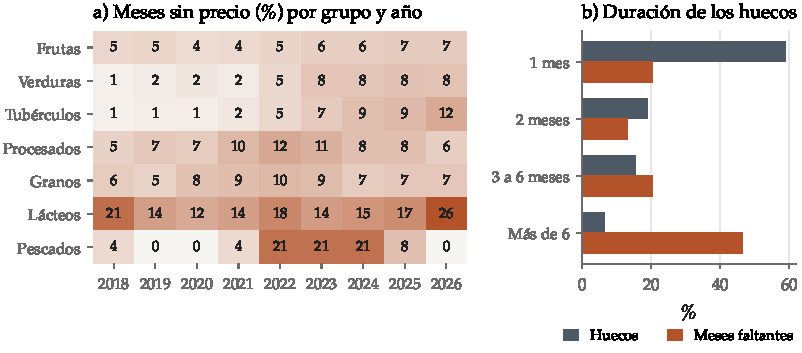
\includegraphics[width=.8\textwidth]{fig_faltantes}
\caption{(a) Porcentaje de meses sin precio por grupo y año, contando desde el primer mes con precio de cada serie. (b) Distribución de la duración de los huecos: porcentaje de huecos y porcentaje de meses faltantes que corresponden a cada duración.}\label{fig:faltantes}
\end{figure}

\subsection*{Tratamiento}

El tratamiento de los faltantes dependió del uso de cada variable (tabla~\ref{tab:falt_tratamiento}). La variable objetivo no se imputó, y las imputaciones de las variables explicativas se hicieron únicamente con información anterior al mes de pronóstico.

\begin{table}[htbp]\centering\small
\caption{Tratamiento de los datos faltantes según su uso}\label{tab:falt_tratamiento}
\begin{tabular}{>{\raggedright\arraybackslash}p{3cm}>{\raggedright\arraybackslash}p{5.1cm}>{\raggedright\arraybackslash}p{4.7cm}}\toprule
Uso & Tratamiento & Razón\\ \midrule
Variable objetivo & Solo precios observados; si falta $p_{t+1}$ la observación se excluye & Una imputación generaría cambios de precio no observados\\
Variables de precio & Se repite el último precio en huecos de hasta dos meses; si el hueco es más largo, la variable queda faltante & El 78\pct\ de los huecos dura uno o dos meses, y la imputación solo usa información pasada\\
SARIMA & Interpolación lineal dentro de la serie con datos hasta el corte & El modelo requiere una serie completa\\
Abastecimiento & Faltante cuando la central no registra el producto & La oferta no observada no puede inferirse\\
Modelos de árboles & El faltante se mantiene (código $-999$ en clasificación) & Los árboles lo tratan como una categoría adicional\\
Modelos lineales y red neuronal & Media de entrenamiento, tras estandarizar & Requieren valores numéricos\\ \bottomrule
\end{tabular}
\end{table}

\subsection*{Mecanismo de pérdida}

El faltante más relevante es el del precio del mes siguiente, porque implica excluir la observación. Esto ocurre en el \cfatasa\pct\ de los casos con precio en el mes actual. Cuando el dato falta, el mismo producto registra en promedio un aumento mayor en las demás centrales (2,8\pct\ frente a 0,8\pct), aunque la proporción de alzas fuertes en las demás centrales es similar (16,6\pct\ frente a 18,0\pct). Por lo tanto, la pérdida no es completamente aleatoria y es algo más frecuente en periodos de aumento de precios, lo que podría excluir algunas alzas del análisis.

\subsection*{Efecto sobre los resultados}

En el periodo de prueba, este tipo de faltante afecta al \cfatasap\pct\ de los casos. En la sección~\ref{sec:res_robustez} se muestra que las conclusiones se mantienen incluso bajo el supuesto de que todos esos casos fueran alzas.

\section{Valores atípicos}
\label{sec:atipicos}

Se marcaron como posibles errores los precios que difieren en un factor mayor a cuatro de la mediana de los siete meses vecinos, umbral orientado a detectar errores de unidad. La ventana es centrada e incluye meses posteriores, de modo que la depuración es retrospectiva; en un uso operativo se aplicaría una regla causal, con la mediana de los meses anteriores. Se identificaron cuatro casos y en cada uno se revisó el comportamiento del mismo producto en las demás centrales. En tres de ellos el movimiento coincidió con el del mercado, como en la espinaca de Corabastos en junio de 2025, que subió junto con otras 16 centrales; estos valores se conservaron. El cuarto caso, las pastas alimenticias de Paloquemao en febrero de 2024, presentó una caída de unas veinte veces sin cambios en otras centrales, por lo que se trató como error de registro y se dejó como faltante. Los cambios grandes que no corresponden a errores se mantuvieron en la muestra. Con un factor de tres la regla marca \rvatcenttres\ casos, de los cuales \rvatcenttresais\ no van acompañados por las demás centrales; con un factor de dos marca \rvatcentdos\ casos (\rvatcentdosais\ aislados), en su mayoría movimientos reales de perecederos. La regla causal con factor de tres marca \rvatcaustres\ casos, \rvatcaustresais\ de ellos aislados. Como el panel tiene \cfilas\ observaciones, estas diferencias no alteran los resultados.

\section{La variable objetivo}
\label{sec:objetivo}

\subsection*{Distribución}

La tabla~\ref{tab:resumen_y} resume el cambio del precio en el mes siguiente. Su media es cercana a cero, con una desviación típica de \csdcambio\ puntos porcentuales y una mediana del cambio absoluto de \cmedabs\ puntos. La mayoría de los cambios son pequeños, pero la distribución presenta colas más pesadas que las de una distribución normal.

\begin{table}[htbp]\centering\small
\caption{Resumen del cambio mensual del precio del mes siguiente ($100\,y$, puntos porcentuales) por grupo: observaciones, media, desviación típica, mínimo, cuartiles, máximo, asimetría y curtosis en exceso}\label{tab:resumen_y}
\begin{adjustbox}{max width=\textwidth}\begin{tabular}{lrrrrrrrrrr}\toprule
Grupo & $n$ & Media & D.\,t. & Mín. & Q1 & Mediana & Q3 & Máx. & Asim. & Curt.\\ \midrule
Todo el panel & 104.354 & 0{,}77 & 19{,}6 & \ensuremath{-}146 & \ensuremath{-}7{,}2 & 0{,}3 & 9{,}1 & 155 & \ensuremath{-}0{,}07 & 3{,}7 \\ \midrule
Frutas & 40.125 & 0{,}95 & 19{,}0 & \ensuremath{-}119 & \ensuremath{-}7{,}3 & 0{,}7 & 9{,}7 & 96 & \ensuremath{-}0{,}16 & 2{,}9 \\
Verduras y hortalizas & 36.067 & 0{,}62 & 24{,}1 & \ensuremath{-}146 & \ensuremath{-}11{,}5 & 0{,}0 & 13{,}2 & 155 & 0{,}00 & 2{,}3 \\
Tubérculos y plátanos & 13.002 & 0{,}83 & 17{,}7 & \ensuremath{-}115 & \ensuremath{-}9{,}0 & 0{,}6 & 10{,}9 & 107 & \ensuremath{-}0{,}20 & 1{,}8 \\
Procesados & 7.916 & 0{,}62 & 4{,}2 & \ensuremath{-}32 & \ensuremath{-}0{,}9 & 0{,}1 & 1{,}8 & 59 & 1{,}38 & 14{,}6 \\
Granos y cereales & 5.815 & 0{,}44 & 5{,}8 & \ensuremath{-}66 & \ensuremath{-}1{,}7 & 0{,}1 & 2{,}3 & 75 & 1{,}01 & 18{,}6 \\
Lácteos y huevos & 1.276 & 0{,}91 & 6{,}5 & \ensuremath{-}34 & \ensuremath{-}1{,}3 & 0{,}3 & 4{,}0 & 24 & \ensuremath{-}0{,}23 & 2{,}5 \\
Pescados & 153 & 0{,}56 & 4{,}8 & \ensuremath{-}15 & \ensuremath{-}1{,}8 & 0{,}1 & 2{,}7 & 15 & 0{,}13 & 1{,}2 \\
\bottomrule\end{tabular}\end{adjustbox}\end{table}


Las diferencias entre grupos de alimentos son marcadas (figuras~\ref{fig:distribucion} y~\ref{fig:cajas}). En verduras, tubérculos y frutas el cambio típico se ubica entre 9 y 12 puntos, mientras que en procesados, granos, lácteos y pescados más de la mitad de los cambios son menores al 2\pct. Las alzas y las caídas fuertes tienen frecuencias similares, lo que indica oscilaciones alrededor de un nivel más que una tendencia sostenida.

\begin{figure}[htbp]\centering
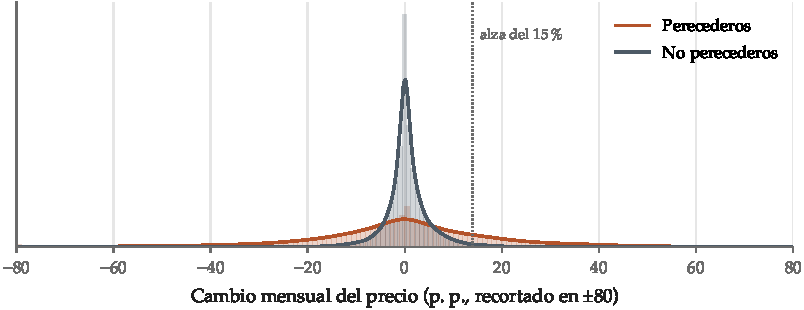
\includegraphics[width=.8\textwidth]{fig_distribucion}
\caption{Distribución del cambio mensual del precio para productos perecederos (frutas, verduras y tubérculos) y no perecederos: histograma y densidad estimada. La línea punteada marca un alza del 15\pct.}\label{fig:distribucion}
\end{figure}

\begin{figure}[htbp]\centering
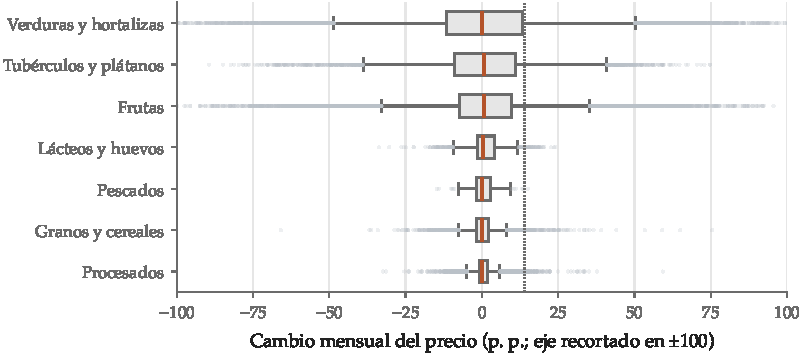
\includegraphics[width=.8\textwidth]{fig_cajas}
\caption{Diagrama de cajas del cambio mensual del precio por grupo de alimentos. La caja va del primer al tercer cuartil y la línea naranja es la mediana; la línea punteada marca un alza del 15\pct.}\label{fig:cajas}
\end{figure}

También hay diferencias importantes entre productos de un mismo grupo (tabla~\ref{tab:volatiles}). El mango Tommy y el limón Tahití registran alzas superiores al 15\pct\ en cerca de cuatro de cada diez meses, mientras que la leche en polvo, la sal y las pastas casi no presentan alzas de esa magnitud.

\begin{table}[htbp]\centering\small
\caption{Los diez productos con mayor y menor cambio mensual típico (mediana del cambio absoluto, p.~p.) y su porcentaje de alzas mayores al 15\,\%, entre los 82 productos con al menos 300 observaciones}\label{tab:volatiles}
\begin{adjustbox}{max width=\textwidth}\begin{tabular}{lrrlrr}\toprule
\multicolumn{3}{c}{Más volátiles} & \multicolumn{3}{c}{Menos volátiles}\\ \cmidrule(lr){1-3}\cmidrule(lr){4-6}
Producto & Cambio & Alzas & Producto & Cambio & Alzas\\ \midrule
Mango Tommy & 27{,}0 & 42 & Leche en polvo & 0{,}5 & 1 \\
Limón Tahití & 26{,}5 & 38 & Sal yodada & 0{,}9 & 1 \\
Pepino cohombro & 23{,}1 & 34 & Pastas alimenticias & 0{,}9 & 0 \\
Cilantro & 20{,}5 & 32 & Sardinas en lata & 1{,}0 & 1 \\
Mango común & 19{,}4 & 33 & Harinas & 1{,}3 & 1 \\
Limón común & 19{,}3 & 33 & Arroz & 1{,}5 & 1 \\
Habichuela & 19{,}2 & 34 & Lenteja & 1{,}9 & 2 \\
Tangelo & 17{,}3 & 30 & Azúcar & 2{,}1 & 3 \\
Mandarina Oneco & 16{,}7 & 29 & Maíz Blanco & 2{,}1 & 2 \\
Pepino de rellenar & 15{,}8 & 29 & Panela & 2{,}4 & 2 \\
\bottomrule\end{tabular}\end{adjustbox}\end{table}


\subsection*{Evolución en el tiempo}

Entre 2019 y 2026 el precio de frutas y tubérculos se duplicó, con un aumento generalizado en 2021 y 2022 (figura~\ref{fig:tiempo}a). La tasa mensual de alzas osciló entre el 8\pct\ y el 36\pct\ (figura~\ref{fig:tiempo}b), con un máximo en mayo de 2021 que coincide con los bloqueos de vías durante el paro nacional.

\begin{figure}[htbp]\centering
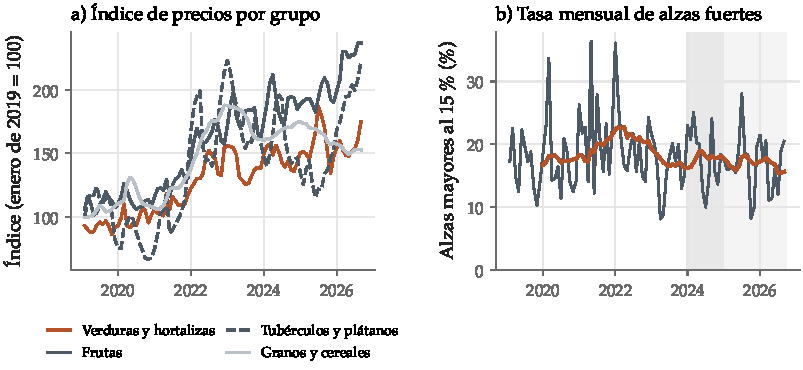
\includegraphics[width=.8\textwidth]{fig_tiempo}
\caption{(a) Índice de precios por grupo, construido encadenando el cambio logarítmico medio de las series de cada grupo. (b) Porcentaje de observaciones con alza mayor al 15\pct\ por mes pronosticado y su promedio móvil de doce meses; sombreado oscuro, validación; claro, prueba.}\label{fig:tiempo}
\end{figure}

En la figura~\ref{fig:anos} se observa que la dispersión del cambio en los perecederos fue estable hasta 2025 y disminuyó en 2026, y que las alzas fueron más frecuentes en 2021 y 2022. Como 2026 solo tiene datos hasta septiembre, la comparación se hizo con los mismos meses (enero a septiembre) de cada año: la desviación típica del cambio en los perecederos osciló entre \rvsdmin\ y \rvsdmax\ puntos de 2019 a 2024, fue de \rvsdveinticinco\ en 2025 y bajó a \rvsdveintiseis\ en 2026. La prueba de Kolmogorov--Smirnov entre desarrollo y prueba, con los mismos meses, rechaza la igualdad de distribuciones en frutas, verduras y granos, aunque con estadísticos pequeños (\rvksfru, \rvksver\ y \rvksgra), que reflejan sobre todo una dispersión menor en la prueba (por ejemplo, de \rvsdfrudes\ a \rvsdfrupru\ puntos en frutas). Un clasificador que intenta distinguir las observaciones de desarrollo y de prueba solo con el cambio del mes siguiente obtiene un AUC de \rvadvy, cercano a 0,5. La prueba es, por tanto, un periodo algo más tranquilo, con la misma forma de distribución.

\begin{figure}[htbp]\centering
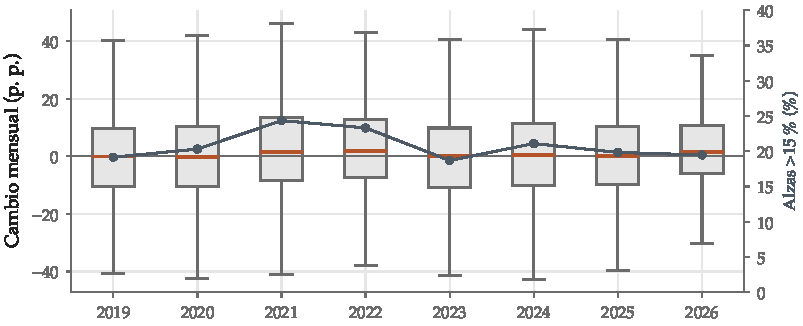
\includegraphics[width=.8\textwidth]{fig_anos}
\caption{Cambio mensual del precio de los productos perecederos por año: diagrama de cajas (sin valores extremos) y porcentaje de alzas mayores al 15\pct\ (línea, eje derecho).}\label{fig:anos}
\end{figure}

\subsection*{Estacionalidad}

La frecuencia de alzas varía según el mes del año y el grupo de alimentos. En verduras las alzas se concentran en diciembre y enero, en tubérculos en marzo y en frutas entre enero y marzo.


A nivel de producto el patrón estacional es aún más definido (figura~\ref{fig:estacional_productos}). La habichuela presenta alzas fuertes en el 72\pct\ de los eneros y la lechuga Batavia en el 65\pct\ de los diciembres, mientras que en otros meses estas alzas son poco frecuentes. Esta heterogeneidad motivó el cálculo de las variables estacionales para cada serie y no solo por grupo.

\begin{figure}[htbp]\centering
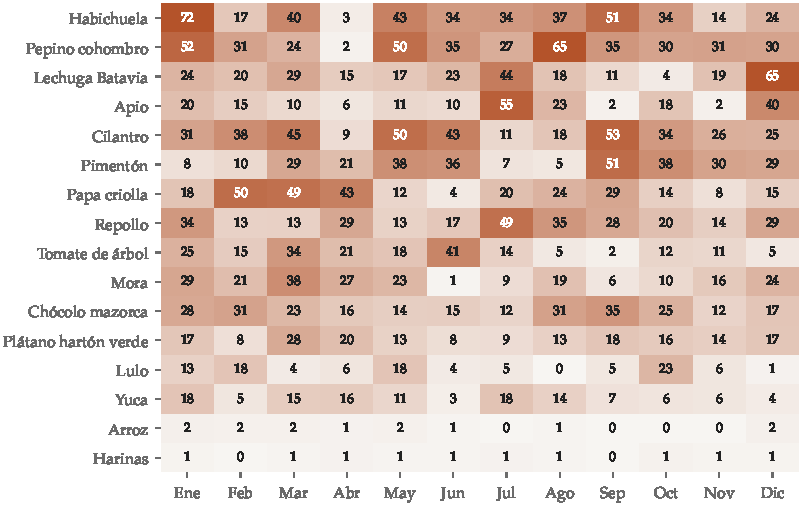
\includegraphics[width=.8\textwidth]{fig_estacional_productos}
\caption{Porcentaje de meses con alza mayor al 15\pct\ por producto y mes del año, para los 16 productos con más observaciones.}\label{fig:estacional_productos}
\end{figure}

\subsection*{Persistencia y autocorrelación}

Los movimientos fuertes tienden a agruparse en el tiempo. En la muestra de entrenamiento, después de un alza mayor al 15\pct\ la probabilidad de una nueva alza fuerte es del 29\pct, aproximadamente el doble que después de un mes sin movimientos grandes (15\pct); de forma simétrica, después de una baja mayor al 15\pct\ la probabilidad de otra baja fuerte es del 28\pct, frente al 12\pct\ después de un mes sin movimientos grandes.

La autocorrelación mediana del cambio mensual es \cacfuno\ en el primer rezago, \cacfdos\ en el segundo y \cacfdoce\ en el rezago doce (figura~\ref{fig:autocorrelacion}a). Este patrón es consistente con choques de oferta de corta duración que se revierten en los meses siguientes, junto con un componente estacional anual. El efecto de promediar las cotizaciones del mes (sección~\ref{sec:economia}) por sí solo produciría una autocorrelación de primer orden cercana a 0,25 si el precio diario siguiera un paseo aleatorio \citep{working1960}; que la observada sea menor indica que, además de ese efecto, parte de los choques se revierte de un mes a otro.

\begin{figure}[htbp]\centering
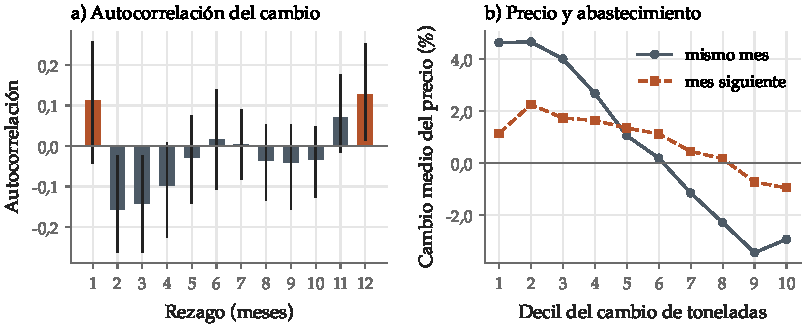
\includegraphics[width=.8\textwidth]{fig_autocorrelacion}
\caption{(a) Autocorrelación del cambio mensual del precio por rezago: mediana entre series y rango intercuartil. (b) Cambio medio del precio en el mismo mes y en el mes siguiente, por decil del cambio de las toneladas que entran a la central.}\label{fig:autocorrelacion}
\end{figure}

El mango Tommy de la Central Mayorista de Antioquia ilustra una serie con estacionalidad fuerte. La descomposición STL \citep{cleveland1990} muestra un ciclo anual con dos picos y una tendencia creciente desde 2021 (figura~\ref{fig:stl}). La fuerza estacional, $F_S=\max\{0,\,1-\operatorname{Var}(R_t)/\operatorname{Var}(S_t+R_t)\}$, con $S_t$ el componente estacional y $R_t$ el residuo \citep{wang2006,fpp3}, es de cerca de 0,8. En consecuencia, la autocorrelación del cambio mensual es alta en los rezagos 6 y 12 (0,44 y 0,56), y también en el rezago 24 (figura~\ref{fig:acf_ejemplo}).

\begin{figure}[htbp]\centering
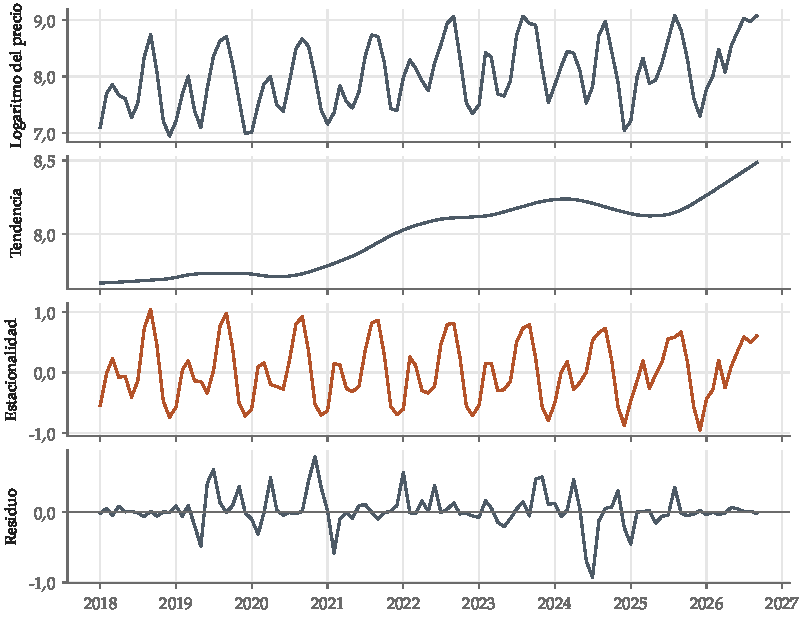
\includegraphics[width=.8\textwidth]{fig_stl}
\caption{Descomposición STL del logaritmo del precio del mango Tommy en la Central Mayorista de Antioquia, 2018--2026: serie, tendencia, estacionalidad y residuo.}\label{fig:stl}
\end{figure}

\begin{figure}[htbp]\centering
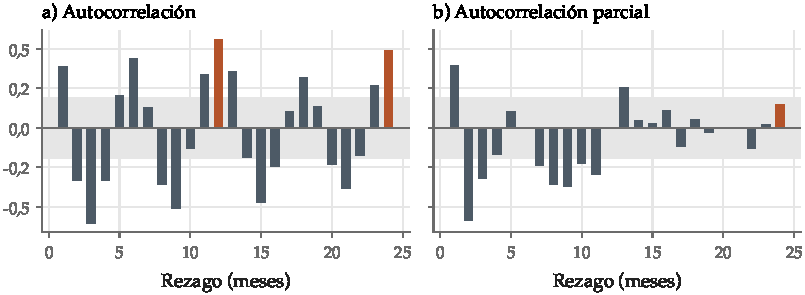
\includegraphics[width=.8\textwidth]{fig_acf_ejemplo}
\caption{Autocorrelación (a) y autocorrelación parcial (b) del cambio mensual del precio del mango Tommy en la Central Mayorista de Antioquia, con banda de no significancia al 95\pct. En naranja, los rezagos 12 y 24.}\label{fig:acf_ejemplo}
\end{figure}

\subsection*{Estacionariedad}

Con la prueba de Dickey--Fuller aumentada \citep{dickey1979} no se rechaza la hipótesis de raíz unitaria en el logaritmo del precio en el \rvadfno\pct\ de las series, mientras que para el cambio mensual se rechaza en casi todas (tabla~\ref{tab:adf}). No rechazar no prueba que exista raíz unitaria, y con unas 84 observaciones por serie la prueba tiene poca potencia. Por eso se complementó con la prueba KPSS \citep{kpss1992}, cuya hipótesis nula es la estacionariedad: esta rechaza en el \rvkpssrech\pct\ de las series, ambas pruebas indican raíz unitaria en el \rvkpssambas\pct\ y ambas indican estacionariedad alrededor de una tendencia en el \rvkpssest\pct. Las pruebas no se ajustaron por multiplicidad, de modo que estas proporciones son descriptivas. La evidencia de raíz unitaria es, entonces, mixta en el nivel y clara a favor de la estacionariedad en el cambio, lo que respalda modelar el cambio del precio.

\begin{table}[htbp]\centering\small
\caption{Pruebas de raíz unitaria (Dickey--Fuller aumentada, $H_0$: raíz unitaria) y de estacionariedad (KPSS, $H_0$: estacionariedad) en las 1.230 series con al menos cinco años de datos, al 5\,\% y sin ajuste por multiplicidad}\label{tab:adf}
\begin{adjustbox}{max width=\textwidth}\begin{tabular}{llr}\toprule
Serie y prueba & Componentes & Series (\%)\\ \midrule
\multicolumn{3}{l}{\emph{Logaritmo del precio}}\\
\quad ADF: no rechaza la raíz unitaria & constante y tendencia & 51{,}5 \\
\quad KPSS: rechaza la estacionariedad & constante y tendencia & 34{,}9 \\
\quad Ambas indican raíz unitaria & & 26{,}6 \\
\quad Ambas indican estacionariedad alrededor de una tendencia & & 40{,}2 \\
\multicolumn{3}{l}{\emph{Cambio mensual}}\\
\quad ADF: rechaza la raíz unitaria & constante & 95{,}7 \\
\quad KPSS: rechaza la estacionariedad & constante & 0{,}7 \\
\bottomrule\end{tabular}\end{adjustbox}\end{table}


\section{Las variables explicativas}
\label{sec:explicativas}

A partir del precio, el abastecimiento y el ONI se construyeron 52 variables candidatas (tabla~\ref{tab:bloques}), cuya definición operativa está en la tabla~\ref{tab:variables} del apéndice. La tabla~\ref{tab:explicativas} resume las principales en la muestra de entrenamiento. Salvo las de abastecimiento, presentan muy pocos faltantes. Su relación individual con el cambio del mes siguiente es débil, con una correlación máxima de 0,27 en valor absoluto, de modo que cualquier ganancia de los modelos dependerá de la combinación de varias variables.

\begin{table}[htbp]\centering\small
\caption{Variables explicativas principales en entrenamiento: porcentaje de faltantes, mediana, cuartiles y correlación de Spearman con el cambio del mes siguiente}\label{tab:explicativas}
\begin{adjustbox}{max width=\textwidth}\begin{tabular}{llrrrrr}\toprule
Variable & Unidad & Faltantes (\%) & Mediana & Q1 & Q3 & $\rho_S$ con $y$\\ \midrule
Cambio del precio, 1 mes & p. p. & 0{,}3 & 0{,}4 & \ensuremath{-}7{,}5 & 9{,}6 & 0{,}101 \\
Cambio del precio, 12 meses & p. p. & 0{,}0 & 10{,}4 & \ensuremath{-}6{,}2 & 28{,}8 & \ensuremath{-}0{,}138 \\
Volatilidad 12 meses & p. p. & 0{,}9 & 15{,}6 & 8{,}9 & 23{,}4 & \ensuremath{-}0{,}004 \\
Distancia al máximo anual & p. p. & 0{,}3 & \ensuremath{-}16{,}9 & \ensuremath{-}39{,}2 & \ensuremath{-}2{,}5 & \ensuremath{-}0{,}182 \\
Frecuencia histórica de alzas en el mes & \% & 0{,}0 & 11{,}0 & 4{,}2 & 25{,}0 & 0{,}183 \\
Cambio histórico en el mes & p. p. & 0{,}0 & 0{,}4 & \ensuremath{-}5{,}4 & 6{,}8 & 0{,}270 \\
Cambio en las demás centrales, 1 mes & p. p. & 0{,}0 & 0{,}7 & \ensuremath{-}5{,}6 & 7{,}5 & 0{,}160 \\
Demás centrales con alza en t & \% & 0{,}0 & 5{,}3 & 0{,}0 & 26{,}1 & 0{,}117 \\
Cambio de toneladas, 1 mes & p. p. & 1{,}6 & 0{,}2 & \ensuremath{-}20{,}5 & 21{,}3 & \ensuremath{-}0{,}051 \\
ONI & \textdegree C & 0{,}0 & \ensuremath{-}0{,}3 & \ensuremath{-}0{,}8 & 0{,}6 & \ensuremath{-}0{,}067 \\
\bottomrule\end{tabular}\end{adjustbox}\end{table}


\subsection*{Abastecimiento}

Las toneladas que ingresan a las centrales muestran un crecimiento gradual y una estacionalidad moderada (figura~\ref{fig:abastecimiento}a). Un mayor volumen se asocia con una leve disminución del precio en el mismo mes (correlación mediana de $-0{,}11$), pero la relación con el precio del mes siguiente es prácticamente nula (figuras~\ref{fig:abastecimiento}b y~\ref{fig:autocorrelacion}b).

\subsection*{Transmisión entre centrales}

El precio del mismo producto en otras centrales presenta la asociación más fuerte con el cambio del precio (figura~\ref{fig:abastecimiento}b). La asociación contemporánea es fuerte (correlación mediana de 0,73) y la adelantada es débil: la correlación mediana con el cambio de las demás centrales en el mes anterior es de 0,20. Esta señal adelantada podría reflejar la autocorrelación del propio precio o el efecto de promediar (sección~\ref{sec:economia}). Sin embargo, en la muestra de entrenamiento la correlación entre el cambio del mes siguiente y el cambio de las demás centrales en el mes actual es de \rvwknac, y controlando por el cambio propio del mes actual baja solo a \rvwkparcial; el cambio propio, en cambio, tiene una correlación de \rvwkpropio. La señal de las demás centrales no se explica, entonces, por la autocorrelación propia.

\begin{figure}[htbp]\centering
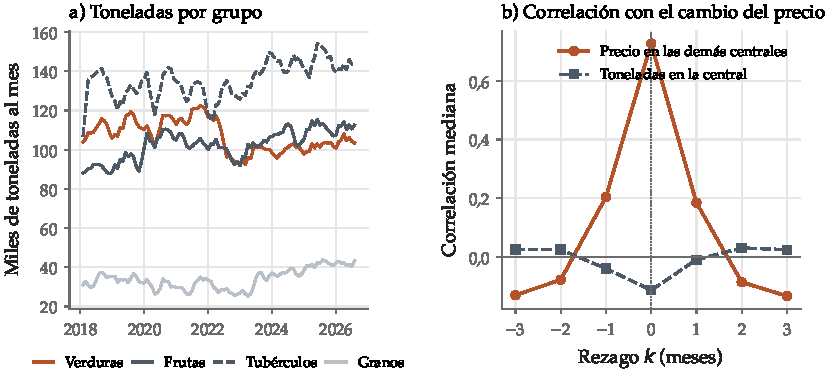
\includegraphics[width=.8\textwidth]{fig_abastecimiento}
\caption{(a) Toneladas mensuales que entran a las centrales del panel por grupo (media móvil de tres meses). (b) Correlación mediana entre series del cambio del precio en el mes $t$ con el cambio en el mes $t+k$ del precio en las demás centrales y de las toneladas en la propia central; $k<0$ indica que la variable va antes que el precio.}\label{fig:abastecimiento}
\end{figure}

\subsection*{El Niño}

Según la serie del ONI usada \citep{noaa} y la clasificación habitual por el valor máximo (débil, de 0,5 a 0,9; moderado, de 1,0 a 1,4; fuerte, de 1,5 a 1,9; muy fuerte, 2,0 o más), entre 2018 y 2026 hubo un episodio moderado de El Niño (2018--2019), uno débil (2019--2020), uno muy fuerte (2023--2024) y otro que comenzó en 2026, además de un periodo prolongado de La Niña entre 2020 y comienzos de 2023. La correlación entre el ONI y la tasa de alzas es cercana a cero para rezagos entre cero y seis meses. Este resultado no excluye efectos del clima a escala regional \citep{bohorquez2026}, pero indica que el índice agregado tiene poca utilidad para pronosticar el mes siguiente.


\subsection*{Correlaciones entre variables}

En la figura~\ref{fig:correlaciones} se observan tres grupos de variables asociadas con el cambio futuro. Las variables estacionales se correlacionan positivamente con él; la posición del precio respecto a su máximo y mínimo del último año se correlaciona negativamente, y el cambio en las demás centrales, positivamente. Algunas variables explicativas están muy correlacionadas entre sí, lo cual se tuvo en cuenta en la selección de variables.

\begin{figure}[htbp]\centering
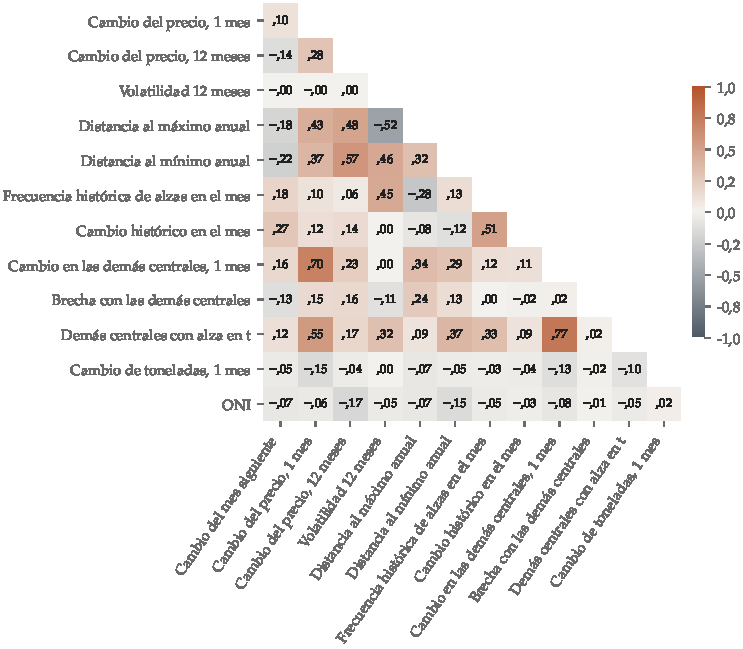
\includegraphics[width=.8\textwidth]{fig_correlaciones}
\caption{Correlaciones de Spearman entre el cambio del mes siguiente y las variables explicativas principales, en la muestra de entrenamiento.}\label{fig:correlaciones}
\end{figure}

\FloatBarrier
\section{Conclusiones del análisis exploratorio}
\label{sec:conclusiones_eda}

Los datos del SIPSA presentan una calidad adecuada para el estudio. Falta el \cfaltserie\pct\ de los precios, en su mayoría en huecos de uno o dos meses, y se identificó un solo error de registro. En el nivel del precio la evidencia de raíz unitaria es mixta, mientras que el cambio mensual es estacionario en casi todas las series, por lo que se modeló el cambio; la presencia de colas pesadas justifica el uso de la pérdida absoluta. Los movimientos grandes se concentran en los productos perecederos, lo que anticipa una capacidad de pronóstico desigual entre grupos. La estacionalidad es marcada y específica de cada producto, por lo que se calcularon variables estacionales por serie. Los movimientos fuertes tienden a agruparse en el tiempo, y el cambio del precio tiene una asociación contemporánea fuerte con el de las demás centrales y una señal adelantada débil. En cambio, ni el abastecimiento de la propia central ni el ONI mostraron relación con el cambio del mes siguiente.

\FloatBarrier

\chapter{Modelado clásico: SARIMA}
\label{cap:sarima}

En este capítulo se desarrolla el segundo objetivo específico: la construcción de un modelo estadístico clásico y la evaluación de su capacidad de pronóstico. Este modelo sirve como referencia para los modelos de aprendizaje automático del capítulo~\ref{cap:ml}.

\section{Justificación del modelo}

El análisis exploratorio mostró que el nivel del precio tiene raíz unitaria en buena parte de las series, que muchas de ellas presentan un ciclo anual y que el cambio de un mes está correlacionado con el de los meses anteriores. El modelo SARIMA \eqref{eq:sarima} incorpora estos tres elementos mediante diferencias regulares y estacionales y términos autorregresivos y de medias móviles, y es el modelo de referencia habitual para series mensuales \citep{box2015}.

\section{Especificación y estimación}

Dado el número de series (1\,260), los órdenes se seleccionaron de forma automática con el procedimiento de \citet{hyndman2008auto}, implementado en la librería statsforecast \citep{garza2022}, que elige para cada serie la especificación con menor criterio de información de Akaike corregido, AICc \citep{hurvich1989}. El número de diferencias regulares se decide con la prueba KPSS y el de diferencias estacionales, con una prueba de estacionalidad. El modelo se estimó sobre el logaritmo del precio con los datos disponibles hasta cada corte, y los huecos se completaron únicamente con información anterior al corte. Durante el pronóstico los parámetros se mantuvieron fijos y el modelo se actualizó con cada nuevo precio observado, al igual que los demás modelos. La probabilidad de alza se calculó sumando al pronóstico los errores históricos de la serie y contando la proporción de casos que superan el 15\pct. Los modelos se estimaron en los tres cortes de validación y en el corte de prueba.

\section{Ejemplo: el mango Tommy en Medellín}

Para el mango Tommy de la Central Mayorista de Antioquia el procedimiento seleccionó un modelo SARIMA$(0,0,1)(0,1,1)_{12}$, con una diferencia estacional y un término de medias móviles regular y otro estacional. Se trata de una especificación habitual en series con un ciclo anual marcado.

Como se observa en la figura~\ref{fig:sarima_ejemplo}, el modelo reproduce el ciclo anual del precio, aunque con cierto retraso en algunos cambios de dirección, y la mayoría de los precios observados se ubica dentro del intervalo del 80\pct. En el periodo de prueba, su error absoluto medio fue de 22,3 puntos, frente a 35,2 del último precio y 19,6 de CatBoost.

\begin{figure}[htbp]\centering
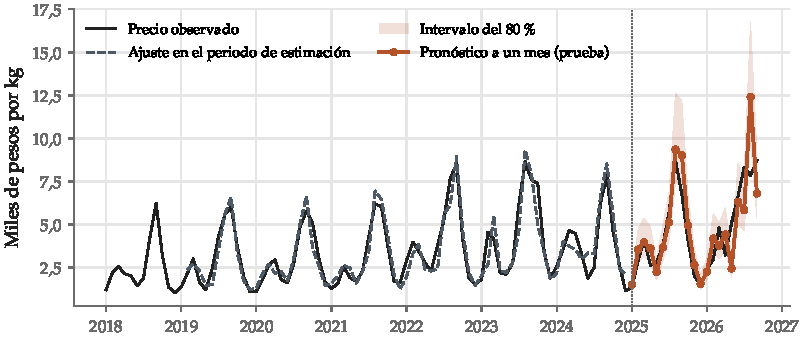
\includegraphics[width=.8\textwidth]{fig_sarima_ejemplo}
\caption{SARIMA$(0,0,1)(0,1,1)_{12}$ para el precio del mango Tommy en la Central Mayorista de Antioquia: ajuste en el periodo de estimación (hasta diciembre de 2024) y pronósticos a un mes en la prueba con un intervalo del 80\pct\ construido con los errores del ajuste.}\label{fig:sarima_ejemplo}
\end{figure}

Los residuos del ajuste oscilan alrededor de cero, sin valores atípicos marcados, sus autocorrelaciones se encuentran dentro de la banda de no significancia al 95\pct\ y la prueba de Ljung--Box \citep{ljung1978} no rechaza la hipótesis de ruido blanco ($p=0{,}39$ con 12 rezagos).


\section{Resultados en el conjunto de series}

La tabla~\ref{tab:sarima} resume las especificaciones seleccionadas con datos hasta 2024. Cerca del 88\pct\ de las series incluyó al menos una diferencia regular, bastante más que el \rvadfno\pct\ en que la prueba de Dickey--Fuller no rechazó la raíz unitaria. La diferencia se debe a que el procedimiento automático decide $d$ con la prueba KPSS sobre la serie en nivel con solo una constante, que rechaza la estacionariedad cuando hay tendencia y, por tanto, tiende a diferenciar más. Solo el 42\pct\ incorporó términos estacionales, posiblemente porque con unos seis años de datos el criterio de información penaliza estos parámetros. En una de cada cuatro series se eligió el modelo $(0,1,0)(0,0,0)$, equivalente al pronóstico con el último precio. Los residuos del \rvlbdoce\pct\ de las series no rechazan la hipótesis de ruido blanco con la prueba de Ljung--Box a 12 rezagos, con grados de libertad ajustados por los parámetros estimados ($12-p-q-P-Q$). Si todos los modelos estuvieran bien especificados se esperaría cerca de un 95\pct, de modo que en unos \rvlbesperado\ puntos porcentuales de las series queda autocorrelación sin capturar.

\begin{table}[htbp]\centering\small
\caption{Modelos SARIMA estimados con datos hasta 2024 (corte de la prueba): órdenes elegidos y diagnóstico de residuos}\label{tab:sarima}
\begin{adjustbox}{max width=\textwidth}\begin{tabular}{lr}\toprule
Característica & Valor\\ \midrule
Series estimadas & 1.260 \\
Con una diferencia regular ($d\ge1$) & 87{,}5\,\% \\
Con diferencia estacional ($D\ge1$) & 12{,}8\,\% \\
Con algún término estacional & 42{,}1\,\% \\
Residuos sin autocorrelación (Ljung--Box, 12 rezagos, $p>0{,}05$) & 84{,}5\,\% \\
Residuos sin autocorrelación (Ljung--Box, 24 rezagos, $p>0{,}05$) & 83{,}7\,\% \\
\midrule
\multicolumn{2}{l}{Órdenes más frecuentes $(p,d,q)(P,D,Q)_{12}$} \\
\quad (0,1,0)(0,0,0) & 24{,}7\,\% \\
\quad (1,1,0)(0,0,0) & 5{,}2\,\% \\
\quad (0,1,1)(0,0,0) & 5{,}0\,\% \\
\quad (2,1,1)(0,0,0) & 3{,}5\,\% \\
\quad (0,1,2)(0,0,0) & 3{,}3\,\% \\
\quad (1,1,1)(0,0,0) & 3{,}1\,\% \\
\bottomrule\end{tabular}\end{adjustbox}\end{table}


En la validación (2022--2024), el error del SARIMA fue mayor que el del último precio en el agregado (tabla~\ref{tab:sarima_error}). El resultado depende del año: en 2022 el SARIMA tuvo un error un \rvsaraabs\pct\ mayor que el último precio, mientras que en 2023 y 2024 lo redujo en un \rvsarb\pct\ y un \rvsarc\pct. En el periodo de prueba redujo el error del último precio en un \cmejsar\pct. La tabla usa la misma definición que la tabla principal de resultados (promedio de los tres años y, donde el SARIMA no pudo estimarse, el último precio; en 2022 se estimó en el \rvsardisp\pct\ de los casos), por lo que sus cifras coinciden con las de la tabla~\ref{tab:reg}. Esta variación entre años indica que la ganancia del modelo depende de la similitud entre el ciclo de los años recientes y el de los años de estimación.

\begin{table}[htbp]\centering\small
\caption{MAE (puntos porcentuales) del último precio y del SARIMA y reducción del error del SARIMA (\%). Validación: promedio de los MAE de 2022, 2023 y 2024, con la misma definición que la tabla~\ref{tab:reg} (donde el SARIMA no pudo estimarse se usa el último precio).}\label{tab:sarima_error}
\begin{adjustbox}{max width=\textwidth}\begin{tabular}{lrrrrrr}\toprule
& \multicolumn{3}{c}{Validación} & \multicolumn{3}{c}{Prueba}\\ \cmidrule(lr){2-4}\cmidrule(lr){5-7}
Grupo & Últ. precio & SARIMA & Reducción & Últ. precio & SARIMA & Reducción\\ \midrule
Todo el panel & 13{,}31 & 13{,}51 & \ensuremath{-}1{,}5 & 12{,}06 & 11{,}50 & 4{,}7 \\ \midrule
Verduras y hortalizas & 17{,}18 & 18{,}04 & \ensuremath{-}5{,}0 & 16{,}33 & 15{,}87 & 2{,}8 \\
Tubérculos y plátanos & 12{,}81 & 14{,}02 & \ensuremath{-}9{,}4 & 12{,}35 & 12{,}16 & 1{,}5 \\
Frutas & 13{,}79 & 12{,}99 & 5{,}8 & 11{,}91 & 10{,}89 & 8{,}6 \\
Lácteos y huevos & 4{,}57 & 4{,}81 & \ensuremath{-}5{,}3 & 3{,}54 & 3{,}54 & 0{,}1 \\
Pescados & 4{,}05 & 5{,}28 & \ensuremath{-}30{,}3 & 3{,}36 & 3{,}95 & \ensuremath{-}17{,}4 \\
Granos y cereales & 3{,}36 & 4{,}22 & \ensuremath{-}25{,}8 & 2{,}75 & 2{,}86 & \ensuremath{-}3{,}8 \\
Procesados & 2{,}54 & 2{,}72 & \ensuremath{-}7{,}0 & 2{,}00 & 2{,}07 & \ensuremath{-}3{,}5 \\
\midrule \multicolumn{7}{l}{\emph{Validación por año (todo el panel)}}\\
\quad 2022 & 13{,}41 & 15{,}93 & \ensuremath{-}18{,}8 & & & \\
\quad 2023 & 12{,}89 & 12{,}01 & 6{,}8 & & & \\
\quad 2024 & 13{,}62 & 12{,}59 & 7{,}6 & & & \\
\bottomrule\end{tabular}\end{adjustbox}\end{table}


\section{Conclusiones del modelado clásico}

El SARIMA presenta un buen ajuste a nivel de serie y reproduce el ciclo anual cuando este es marcado. No obstante, su mejora frente al último precio es pequeña y varía entre periodos. Dos limitaciones explican este resultado: cada modelo utiliza únicamente la historia de su propia serie y, con pocos años de datos, los componentes estacionales se estiman con baja precisión. Estos resultados motivan el uso de modelos que aprovechen la información conjunta de todas las series.

\FloatBarrier

\chapter{Modelado con aprendizaje automático}
\label{cap:ml}

En este capítulo se desarrollan el tercer y el cuarto objetivo específico. Se construyen los modelos de aprendizaje automático, se comparan con los modelos de referencia bajo las mismas condiciones y se evalúa la utilidad de las alertas de alza.

\section{Planteamiento}
\label{sec:planteamiento}

\subsection{Horizonte de pronóstico y fuga de información}
\label{sec:fuga}

Los modelos se utilizan al cierre de cada mes para pronosticar el mes siguiente, por lo que todas las variables explicativas deben calcularse con la información disponible en ese momento. Las variables se construyeron a partir de la matriz de logaritmos de precios y, solo para este fin, los huecos de hasta dos meses se completaron con el último precio observado. Se agruparon en los bloques de la tabla~\ref{tab:bloques}:
\begin{itemize}[nosep]
\item \emph{Historia del precio}: cambios acumulados $\ln p_t-\ln p_{t-k}$ para $k=1,2,3,6,12$; cambios de los tres meses anteriores; volatilidad en ventanas de 3, 6 y 12 meses; posición del precio en el último año, $z_t=(\ln p_t-\bar\ell_{12})/s_{12}$, y distancia al máximo y al mínimo anual; número de alzas en el último año y meses desde la última.
\item \emph{Estacionalidad}: mes del año en forma de seno y coseno; frecuencia histórica de alzas del producto en ese mes, y cambio medio de la serie en ese mes en los años anteriores.
\item \emph{Red de centrales}: diferencia entre el precio de la central y el promedio del producto en las demás centrales, cambio de ese promedio y proporción de centrales con alza mayor al 15\pct\ en $t$.
\item \emph{Producto y lugar}: grupo, producto, central, ciudad e indicador de perecibilidad.
\end{itemize}
La tabla~\ref{tab:variables} del apéndice da la fórmula y la ventana de cada una de las 52 variables candidatas.

Para evitar la fuga de información, todos los rezagos se calcularon hacia atrás, la frecuencia y el cambio histórico de cada mes del año se calcularon solo con años anteriores al pronosticado, las variables de red excluyen a la propia central y el ONI se incluyó con dos meses de rezago, que corresponden a su tiempo de publicación.

Hay que precisar qué significa \emph{anticipar}. El boletín mensual del SIPSA se publica el día hábil siguiente a la divulgación del IPC \citep{danefme2022}, unos ocho días después de terminar el mes; el de septiembre de 2026, por ejemplo, salió el 8 de octubre \citep{danebol2026}. Con el boletín mensual, el pronóstico del mes $t+1$ solo puede hacerse cuando ya ha transcurrido cerca de una cuarta parte de ese mes, y la variable objetivo es el promedio de todo el mes $t+1$. El horizonte efectivo es, por tanto, algo menor a un mes. Hay dos formas de recuperar el horizonte completo: construir las variables con los boletines semanales o diarios del SIPSA, que se publican durante el mes, o pronosticar el cambio entre $t+1$ y $t+2$ con la información de $t$. La segunda se evalúa en la sección~\ref{sec:res_robustez}; la primera queda como trabajo futuro, porque requiere los archivos semanales, que no se descargaron para este estudio.

\subsection{Definición de alza}

Se definió como alza fuerte un aumento del precio superior al 15\pct\ de un mes a otro ($y>\ln 1{,}15$). Este umbral es convencional y no se derivó de los costos de un usuario particular; se eligió para distinguir los movimientos grandes, con efecto en las decisiones de compra, de las variaciones habituales. Con esta definición, cerca del 18\pct\ de las observaciones corresponde a alzas, lo que implica un desbalance de clases moderado.

\subsection{Esquema de validación temporal}
\label{sec:esquema}

La figura~\ref{fig:cortes} muestra el uso de los datos en el tiempo. Para elegir los hiperparámetros, cada configuración se estimó con datos hasta 2021, 2022 y 2023 y se evaluó en el año siguiente, y se usó como criterio el promedio de los tres años, que es más estable que el resultado de un solo año. La selección de variables utilizó los cortes de 2023 y 2024. Una vez tomadas todas las decisiones, cada modelo se estimó con los datos de 2019 a 2024 y se usó para pronosticar los 21 meses del periodo de prueba sin reestimarse.

\begin{figure}[htbp]\centering
\begin{tikzpicture}[x=1.45cm, y=.55cm, every node/.style={font=\footnotesize}]
\foreach \a in {2019,...,2026} { \node[anchor=south] at (\a-2019+.5, 4.55) {\a}; }
\foreach \a in {0,...,8} { \draw[black!25] (\a, .2) -- (\a, 4.5); }
\def\fila#1#2#3#4{ \fill[black!18] (0,#1) rectangle (#2,#1+.62); \fill[orange!70!brown] (#2,#1) rectangle (#3,#1+.62); \node[anchor=east] at (-.1,#1+.31) {#4}; }
\fila{3.6}{3}{4}{Corte 1}
\fila{2.8}{4}{5}{Corte 2}
\fila{2.0}{5}{6}{Corte 3}
\fill[black!18] (0,.6) rectangle (6,1.22); \fill[orange!45!brown] (6,.6) rectangle (7.75,1.22); \node[anchor=east] at (-.1,.91) {Prueba};
\fill[black!18] (0.2,-.6) rectangle (.6,-.25); \node[anchor=west] at (.65,-.42) {estimación};
\fill[orange!70!brown] (2.2,-.6) rectangle (2.6,-.25); \node[anchor=west] at (2.65,-.42) {evaluación};
\end{tikzpicture}
\caption{Cortes temporales. Los cortes 1 a 3 sirven para elegir hiperparámetros, balanceo, umbral y modelo; los cortes 2 y 3, para seleccionar variables. La prueba se evalúa una sola vez.}\label{fig:cortes}
\end{figure}

\subsection{Modelos y búsqueda de hiperparámetros}
\label{sec:ajuste}

La tabla~\ref{tab:modelos} presenta los modelos comparados, todos ellos individuales. Los seis modelos de aprendizaje automático y el AR estacional minimizan la misma pérdida en cada tarea (absoluta para el cambio y logarítmica para las alzas), y los seis primeros siguen la misma regla de búsqueda de hiperparámetros. Las demás referencias no comparten esa pérdida: el SARIMA se estima por máxima verosimilitud gaussiana, el paseo aleatorio no estima parámetros y la frecuencia histórica es una proporción suavizada.

Las variables categóricas no entran igual en todos los modelos (tabla~\ref{tab:codificacion}). En los modelos de árboles, el grupo, el producto, la central y la ciudad entran como códigos enteros, que los árboles pueden partir en intervalos; CatBoost recibe esos mismos códigos como variables numéricas, sin su tratamiento propio de variables categóricas. En la regresión lineal y la red neuronal, que no pueden interpretar un código entero, entra solo el grupo como indicadores, junto con la perecibilidad. Como esta diferencia podría favorecer a los árboles, en la sección~\ref{sec:res_robustez} se reestiman los modelos lineales y la red con indicadores de producto, central y ciudad.

\begin{table}[htbp]\centering\small
\caption{Tratamiento de las variables en cada familia de modelos}\label{tab:codificacion}
\begin{tabular}{>{\raggedright\arraybackslash}p{3.1cm}>{\raggedright\arraybackslash}p{4.4cm}>{\raggedright\arraybackslash}p{5.3cm}}\toprule
Modelos & Variables numéricas & Grupo, producto, central y ciudad\\ \midrule
Random Forest, XGBoost, LightGBM y CatBoost & Escala original; faltantes como tales (regresión) o con el código $-999$ (clasificación) & Códigos enteros asignados en orden alfabético\\
Regresión cuantílica, regresión logística y MLP & Estandarizadas con la media y la desviación de los datos de ajuste; faltantes iguales a 0 tras estandarizar & Solo el grupo, como indicadores (\emph{one-hot}); producto, central y ciudad no entran\\
AR estacional y logística autorregresiva & Rezagos del cambio por grupo & Efectos de grupo y de mes por grupo\\ \bottomrule
\end{tabular}
\end{table}

\begin{table}[htbp]\centering\small
\caption{Modelos comparados}\label{tab:modelos}
\begin{tabular}{l>{\raggedright\arraybackslash}p{4.7cm}>{\raggedright\arraybackslash}p{4.7cm}}\toprule
Tipo & Cambio del mes siguiente & Alzas mayores al 15\,\%\\ \midrule
Referencias & Paseo aleatorio, AR estacional, SARIMA & Frecuencia histórica, logística autorregresiva, SARIMA\\
Lineal & Regresión cuantílica (mediana) & Regresión logística\\
Red neuronal & MLP & MLP\\
Promedio de árboles & Random Forest & Random Forest\\
Potenciación & XGBoost, LightGBM, CatBoost & XGBoost, LightGBM, CatBoost\\ \bottomrule
\end{tabular}
\end{table}

Tres modelos requirieron implementaciones propias, ya que las librerías utilizadas no los ofrecen con la pérdida absoluta o resultan demasiado lentas para el tamaño de la muestra. La red neuronal con pérdida absoluta se programó en NumPy; la regresión cuantílica se estimó por descenso de gradiente estocástico, y el Random Forest con pérdida absoluta se implementó con el modo de bosque de LightGBM, que no es idéntico al algoritmo de \citet{breiman2001}. Las tres implementaciones se verificaron frente a versiones de referencia (apéndice~\ref{ap:modelos}).

Los hiperparámetros se eligieron mediante búsqueda aleatoria con la regla de parada \eqref{eq:convergencia}, con 40 configuraciones iniciales, ampliaciones de 20 hasta un máximo de 100 y tolerancias de 0,01 puntos de MAE y 0,002 de AP. La tabla~\ref{tab:espacios} muestra los rangos explorados. Todas las búsquedas se detuvieron con las 40 configuraciones iniciales, salvo la de XGBoost en regresión, que se amplió a 60 porque su mejor configuración apareció en la posición 39; así, el presupuesto de evaluaciones fue el mismo para todos los modelos excepto ese. Un presupuesto igual no implica el mismo grado de exploración: cuarenta configuraciones cubren bien un espacio de uno o dos hiperparámetros, pero solo parcialmente uno de siete. La figura~\ref{fig:busqueda} del apéndice muestra que, al detenerse cada búsqueda, la mejora en las últimas configuraciones fue menor que la tolerancia. En el ajuste final con 2019--2024, el número de árboles o de iteraciones es el elegido en validación, sin reescalarlo por el mayor tamaño de la muestra, y la red neuronal usa parada temprana con un 10\pct\ aleatorio de las filas de ajuste.

\begin{table}[htbp]\centering\small
\caption{Espacios de búsqueda de los hiperparámetros. Los rangos continuos se sortean en escala logarítmica cuando se indica (log).}\label{tab:espacios}
\begin{tabular}{l>{\raggedright\arraybackslash}p{10.1cm}}\toprule
Modelo & Hiperparámetros y rangos\\ \midrule
Regresión cuantílica & penalización $\alpha\in[10^{-7},10^{-2}]$ (log), tipo $L_1$ o $L_2$\\
Regresión logística & inverso de la penalización $C\in[10^{-3},10]$ (log), tipo $L_1$ o $L_2$\\
MLP & capas $\{(32),(64),(64,32),(128,64)\}$; penalización $[10^{-6},10^{-2}]$ (log); tasa de aprendizaje $[10^{-4},3\cdot10^{-3}]$ (log); hasta 80 épocas con parada temprana\\
Random Forest & 200 árboles (regresión) o 250 (clasificación); profundidad 8 a 19; hoja mínima 10 a 149; fracción de variables por división 0,3 a 0,8\\
XGBoost & árboles 150 a 599; tasa 0,02 a 0,12 (log); profundidad 3 a 8; peso mínimo por hoja 1 a 60 (log); submuestra 0,6 a 1; fracción de columnas 0,4 a 1\\
LightGBM & árboles 150 a 699; tasa 0,02 a 0,12 (log); hojas 8 a 96; observaciones por hoja 20 a 399; submuestra 0,6 a 1; fracción de columnas 0,4 a 1; regularización $\lambda\in[10^{-3},10]$ (log)\\
CatBoost & iteraciones 250 a 549; profundidad 4 a 8; tasa 0,02 a 0,12 (log); regularización $\lambda\in[1,10]$ (log)\\ \bottomrule
\end{tabular}
\end{table}

Con los hiperparámetros elegidos, cada clasificador se estimó de tres formas: sin balanceo, con un peso $(1-\bar z)/\bar z$ para las alzas y con submuestreo de los casos sin alza. Se estableció que un método de balanceo se adoptaría solo si aumentaba la AP de validación en más de 0,005. Las predicciones de los tres cortes se reunieron en una muestra de validación de 36 meses, que se utilizó para corregir las probabilidades (sección~\ref{sec:metricas}), fijar el umbral que maximiza $F_1$ y elegir el modelo de cada tarea. Como esos años se usaron para varias decisiones (selección de variables, hiperparámetros, recalibración, umbral y elección del modelo), las métricas de validación de este capítulo son optimistas; la única evaluación imparcial es la de la prueba. El análisis según los costos se realizó con el beneficio neto \eqref{eq:bn}.


\FloatBarrier
\section{Selección de variables}
\label{sec:seleccion}

La selección de variables se realizó con LightGBM, con hiperparámetros fijos y predicciones promediadas sobre tres semillas, a partir de los pronósticos de 2023 y 2024. Cada cambio se evaluó con el intervalo bootstrap por meses de la diferencia de MAE y de AP respecto a la configuración de partida. El procedimiento tuvo tres etapas:
\begin{enumerate}[nosep]
\item \emph{Bloques.} Un bloque nuevo se incorpora si mejora significativamente una tarea sin empeorar la otra, y un bloque de partida se retira si su exclusión no empeora significativamente ninguna. La historia del precio y el bloque de producto y lugar se mantienen en todos los casos.
\item \emph{Variables poco informativas.} Se retiran en conjunto las variables cuya importancia por permutación no supera dos desviaciones típicas en ninguna de las dos tareas, siempre que su exclusión no empeore el desempeño.
\item \emph{Redundancia.} En cada par de variables con correlación de Spearman igual o superior a 0,85 se evalúa la exclusión de la menos importante con el mismo criterio.
\end{enumerate}
El criterio es deliberadamente asimétrico, ya que una variable se incorpora solo con evidencia de mejora y se retira cuando no hay evidencia de deterioro, lo que favorece modelos más simples. Las comparaciones no se ajustaron por multiplicidad. Como la selección se hizo con un modelo de árboles, el conjunto final podría favorecer a esa familia; la sección~\ref{sec:res_robustez} evalúa los modelos lineales y la red con las 52 candidatas.

\begin{table}[htbp]\centering\small
\caption{Bloques de variables candidatas y resultado de la selección. Arriba, los bloques de partida; abajo, los bloques adicionales evaluados.}\label{tab:bloques}
\begin{adjustbox}{max width=\textwidth}\begin{tabular}{l>{\raggedright\arraybackslash}p{5.6cm}rrl}\toprule
Bloque & Contenido & Candidatas & Finales & Decisión\\ \midrule
Historia del precio & cambios acumulados y rezagados, volatilidad, posición en el rango anual & 16 & 14 & Queda en parte \\
Estacionalidad & mes del año, frecuencia y cambio histórico del mismo mes & 4 & 4 & Queda \\
Abastecimiento local & toneladas ingresadas, municipios de origen, días con registro & 6 & 0 & Sale \\
Red de centrales & precio del producto en las demás centrales & 3 & 3 & Queda \\
Calendario & Semana Santa, diciembre & 2 & 0 & Sale \\
Producto y lugar & grupo, producto, central, ciudad, perecibilidad & 5 & 5 & Queda \\
El Niño (ONI) & índice ONI y su cambio & 2 & 0 & Sale \\
\midrule
Promedios móviles & distancia a medias móviles & 2 & 0 & No entra \\
Año anterior & cambio del mismo mes un año antes & 2 & 0 & No entra \\
Red ampliada & otros cambios del precio nacional & 3 & 0 & No entra \\
Grupo en la central & cambio y alzas del grupo en la central & 2 & 0 & No entra \\
Abastecimiento nacional & toneladas nacionales y participación de la central & 3 & 3 & Queda \\
Calidad del dato & meses y días con registro & 2 & 0 & No entra \\
\bottomrule\end{tabular}\end{adjustbox}\end{table}


El procedimiento redujo las 52 variables candidatas a \cnfinal\ (tabla~\ref{tab:bloques}). En la figura~\ref{fig:bloques} se observa que los bloques con mayor aporte son la estacionalidad, cuya exclusión aumenta el MAE de validación en 0,49 puntos, y la red de centrales, con un aumento de 0,13 puntos. Se retiraron el abastecimiento de la propia central, el calendario y El Niño, y se incorporó el abastecimiento nacional (toneladas del producto en todas las centrales y participación de la central), el único bloque adicional con una mejora significativa. En la segunda etapa no se retiró ninguna variable y en la tercera se retiraron, por redundancia, la volatilidad de seis meses y el número de alzas del último año. Ninguna etapa modificó el desempeño de forma significativa (tabla~\ref{tab:pasos}).

La selección es sensible a cambios pequeños en los datos. Con la versión de la base anterior a la corrección de la variedad de referencia (sección~\ref{sec:carga}), que difería en una sola serie, el procedimiento había elegido 24 variables: incorporaba en la primera etapa el bloque de calidad del dato en lugar del abastecimiento nacional (y luego retiraba sus dos variables), y retiraba el cambio de tres meses y la volatilidad de tres meses. Los efectos de ambos bloques eran casi iguales (reducciones del MAE de validación de 0,02 a 0,03 puntos) y quedaban a uno y otro lado del criterio de significancia. Las cinco variables adicionales de la versión actual concentran, en conjunto, el 6\pct\ del aporte a los pronósticos de regresión y el 10\pct\ en clasificación según los valores de Shapley (sección~\ref{sec:res_importancia}), y el error en la prueba prácticamente no cambió (MAE de \cmaee\ con 29 variables frente a 10,58 con 24).

\begin{figure}[htbp]\centering
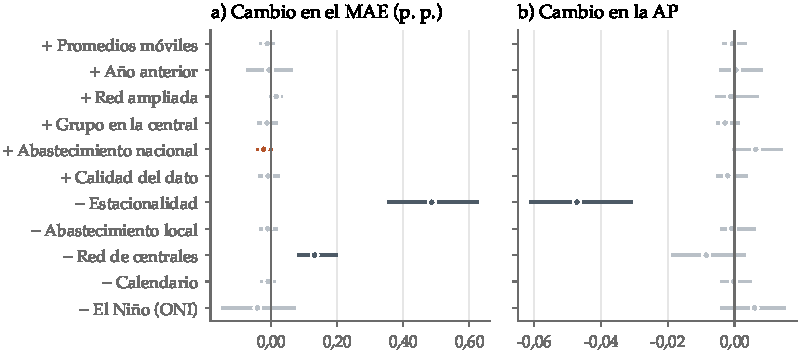
\includegraphics[width=.8\textwidth]{fig_bloques}
\caption{Efecto de añadir (+) o quitar ($-$) cada bloque de variables sobre el MAE (a) y la AP (b) en las predicciones de 2023 y 2024, con intervalos bootstrap del 95\pct. En naranja, mejoras significativas; en gris oscuro, empeoramientos significativos; en gris claro, efectos no significativos.}\label{fig:bloques}
\end{figure}

\begin{table}[htbp]\centering\small
\caption{Desempeño de LightGBM en las predicciones de 2023 y 2024 después de cada etapa de la selección, y diferencia frente a las 38 variables de partida con su intervalo del 95\,\%}\label{tab:pasos}
\begin{adjustbox}{max width=\textwidth}\begin{tabular}{lrrrrr}\toprule
Etapa & Variables & MAE & Diferencia & AP & Diferencia\\ \midrule
Partida & 38 & 11{,}23 & 0{,}000 [0{,}000; 0{,}000] & 0{,}520 & 0{,}000 [0{,}000; 0{,}000] \\
Todas las candidatas & 52 & 11{,}22 & \ensuremath{-}0{,}006 [\ensuremath{-}0{,}060; 0{,}054] & 0{,}523 & 0{,}003 [\ensuremath{-}0{,}003; 0{,}013] \\
Etapa 1: bloques & 31 & 11{,}19 & \ensuremath{-}0{,}034 [\ensuremath{-}0{,}146; 0{,}079] & 0{,}531 & 0{,}011 [\ensuremath{-}0{,}002; 0{,}024] \\
Etapa 2: sin poco informativas & 31 & 11{,}19 & \ensuremath{-}0{,}034 [\ensuremath{-}0{,}146; 0{,}079] & 0{,}531 & 0{,}011 [\ensuremath{-}0{,}002; 0{,}024] \\
Etapa 3: sin redundancias (final) & 29 & 11{,}18 & \ensuremath{-}0{,}047 [\ensuremath{-}0{,}156; 0{,}063] & 0{,}532 & 0{,}012 [0{,}000; 0{,}025] \\
\bottomrule\end{tabular}\end{adjustbox}\end{table}



\section{Resultados para el cambio del mes siguiente}
\label{sec:res_reg}

\subsection{Entrenamiento, validación y prueba}

La tabla~\ref{tab:entrenamiento} presenta el desempeño de cada modelo en las muestras de entrenamiento, validación y prueba. Debido a que los precios fueron más volátiles entre 2019 y 2024 que en el periodo de prueba, la comparación se hace con la reducción del error frente al último precio. En los modelos lineales esta reducción es similar en las tres muestras. En los modelos de árboles, en cambio, pasa de 23--28\pct\ en entrenamiento a cerca del 12\pct\ en prueba, y en la clasificación la AP del Random Forest baja de 0,76 a 0,49. A pesar de ese sobreajuste en entrenamiento, los modelos de árboles tienen el menor error en validación y en prueba; elegir los hiperparámetros en validación controla el sobreajuste, pero no lo elimina.

\begin{table}[htbp]\centering\small
\caption{Desempeño en entrenamiento (ajuste y evaluación con 2019--2024), validación (promedio de 2022--2024 en regresión; predicciones reunidas en clasificación) y prueba. Una diferencia grande entre entrenamiento y prueba indica sobreajuste. Las cifras de validación son optimistas, porque esa muestra se usó para varias decisiones; la única evaluación imparcial es la de prueba.}\label{tab:entrenamiento}
\begin{adjustbox}{max width=\textwidth}\begin{tabular}{lrrr}\toprule
Modelo & Entrenamiento & Validación & Prueba\\ \midrule
\multicolumn{4}{l}{\emph{Cambio del mes siguiente: MAE (p. p.)}}\\
Paseo aleatorio & 13{,}40 & 13{,}31 & 12{,}06 \\
AR estacional & 12{,}33 & 12{,}34 & 11{,}47 \\
Regresión cuantílica & 11{,}95 & 11{,}92 & 11{,}07 \\
MLP & 11{,}35 & 11{,}44 & 10{,}67 \\
Random Forest & 9{,}89 & 11{,}56 & 10{,}69 \\
XGBoost & 9{,}65 & 11{,}38 & 10{,}60 \\
LightGBM & 9{,}83 & 11{,}40 & 10{,}59 \\
CatBoost$^\ast$ & 10{,}30 & 11{,}33 & 10{,}59 \\
\midrule
\multicolumn{4}{l}{\emph{Alzas mayores al 15\,\%: AP}}\\
Logística autorregresiva & 0{,}430 & -- & 0{,}381 \\
Regresión logística & 0{,}490 & 0{,}502 & 0{,}465 \\
MLP & 0{,}571 & 0{,}504 & 0{,}485 \\
Random Forest & 0{,}760 & 0{,}521 & 0{,}490 \\
XGBoost & 0{,}658 & 0{,}520 & 0{,}495 \\
LightGBM & 0{,}732 & 0{,}523 & 0{,}492 \\
CatBoost$^\ast$ & 0{,}594 & 0{,}524 & 0{,}481 \\
\bottomrule\end{tabular}\end{adjustbox}\end{table}


\subsection{Comparación con los modelos de referencia}

CatBoost obtuvo el menor error en validación y fue el modelo seleccionado. En el periodo de prueba redujo el error del último precio en un \cmeje\pct, con un intervalo de confianza del 95\pct\ entre \cmejloe\pct\ y \cmejhie\pct\ (tabla~\ref{tab:reg}). Su error fue menor en \cmesesgana\ de los \cnmeses\ meses y en el \cseriese\pct\ de las series, y la prueba de Diebold--Mariano rechaza la igualdad de errores ($p<0{,}001$ con el ajuste de Holm), con lo que se acepta la hipótesis H1. La reducción supera también la referencia de relevancia práctica del 5\pct\ planteada en la sección~\ref{sec:hipotesis}.

\begin{table}[htbp]\centering\small
\caption{Pronóstico del cambio del mes siguiente. Error absoluto medio (MAE, en puntos porcentuales) en validación (2022--2024) y en prueba (enero de 2025 a septiembre de 2026), reducción del error frente al último precio y diferencia de MAE con CatBoost (positiva: peor que CatBoost). Entre corchetes, intervalos al 95\,\%; los de la última columna están ajustados por comparaciones múltiples. $^\ast$Modelo elegido.}\label{tab:reg}
\begin{adjustbox}{max width=\textwidth}\begin{tabular}{lrrrr}\toprule
& \multicolumn{2}{c}{MAE} & Reducción del & Diferencia \\ \cmidrule(lr){2-3}
Modelo & Validación & Prueba & error (\%) & con CatBoost\\ \midrule
Paseo aleatorio & 13{,}31 & 12{,}06 & -- & 1{,}48 [0{,}72; 2{,}32] \\
AR estacional & 12{,}34 & 11{,}47 & 4{,}9 [3{,}5; 7{,}0] & 0{,}88 [0{,}35; 1{,}42] \\
SARIMA & 13{,}51 & 11{,}50 & 4{,}7 [1{,}5; 7{,}7] & 0{,}91 [0{,}54; 1{,}47] \\
\midrule
Regresión cuantílica & 11{,}92 & 11{,}07 & 8{,}2 [5{,}0; 12{,}5] & 0{,}48 [0{,}28; 0{,}68] \\
MLP & 11{,}44 & 10{,}67 & 11{,}5 [8{,}0; 15{,}8] & 0{,}09 [0{,}00; 0{,}20] \\
Random Forest & 11{,}56 & 10{,}69 & 11{,}4 [8{,}7; 14{,}8] & 0{,}10 [\ensuremath{-}0{,}14; 0{,}38] \\
XGBoost & 11{,}38 & 10{,}60 & 12{,}2 [8{,}4; 16{,}6] & 0{,}01 [\ensuremath{-}0{,}04; 0{,}08] \\
LightGBM & 11{,}40 & 10{,}59 & 12{,}2 [8{,}3; 16{,}8] & 0{,}00 [\ensuremath{-}0{,}04; 0{,}06] \\
CatBoost$^\ast$ & 11{,}33 & 10{,}59 & 12{,}2 [8{,}3; 16{,}9] & -- \\
\bottomrule\end{tabular}\end{adjustbox}\end{table}


En la figura~\ref{fig:modelos}a se distinguen tres grupos de modelos. Los cinco modelos no lineales reducen el error entre un 11,4\pct\ y un 12,2\pct. Las diferencias entre los cuatro modelos de árboles no son significativas; la red neuronal tiene un error \cdmlp\ puntos mayor que CatBoost, una diferencia pequeña pero significativa. La regresión cuantílica alcanza una reducción del \cmejlin\pct, y los modelos de referencia se ubican alrededor del 5\pct\ (\cmejar\pct\ el AR estacional y \cmejsar\pct\ el SARIMA). El error de CatBoost es \cdar\ puntos menor que el del AR estacional y \cdsar\ puntos menor que el del SARIMA, diferencias significativas después del ajuste por comparaciones múltiples.

\begin{figure}[htbp]\centering
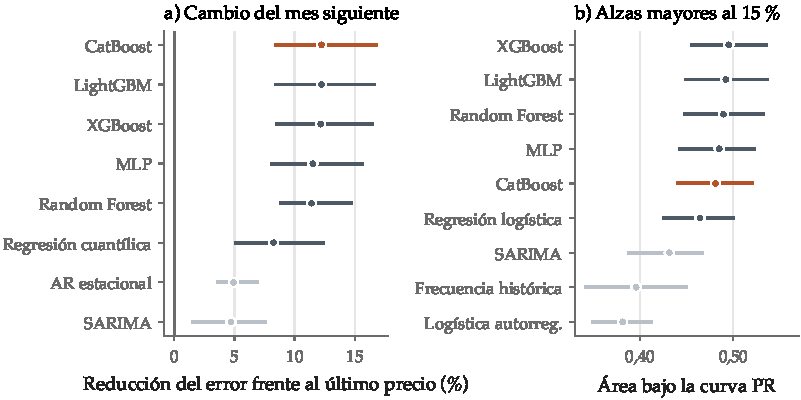
\includegraphics[width=.8\textwidth]{fig_modelos}
\caption{Desempeño en la prueba con intervalos de confianza del 95\pct. (a) Reducción del error absoluto medio frente al último precio. (b) Área bajo la curva de precisión y exhaustividad; un modelo sin información obtendría \ctasaprueba\pct, la tasa de alzas. En naranja, el modelo elegido; en gris claro, las referencias.}\label{fig:modelos}
\end{figure}

Al comparar el cambio pronosticado con el observado en la prueba, la dispersión es alta, lo que indica que una parte importante del cambio mensual no es predecible con estas variables. Sin embargo, la mediana del cambio observado sigue de cerca al pronóstico en todo el rango, aunque con magnitudes algo menores en los extremos.


La mejora varía entre grupos de alimentos (figura~\ref{fig:grupos}). Es significativa en frutas (\cgfru\pct) y verduras (\cgver\pct), que representan tres cuartas partes de los pronósticos. En tubérculos (\cgtub\pct), procesados (\cgpro\pct) y lácteos (\cglac\pct) no es significativa, y en granos y pescados es prácticamente nula. Si cada grupo pesa lo mismo, el resultado depende de cómo se agregue: la razón entre el MAE promedio de los siete grupos y el del último precio, $1-\overline{\mathrm{MAE}}_g/\overline{\mathrm{MAE}}_{\mathrm{PA},g}$, da una reducción del \rvrazongrupos\pct\ con CatBoost y del \rvrazongruposlin\pct\ con la regresión cuantílica, mientras que el promedio simple de las siete reducciones da \rvredgrupos\pct\ y \rvredgruposlin\pct. La segunda medida es más exigente porque da el mismo peso a grupos con muy pocos pronósticos, como pescados. La tabla~\ref{tab:grupos_modelos} muestra que en frutas todos los modelos de aprendizaje automático, incluido el lineal, alcanzan reducciones del 18--19\pct, mientras que en tubérculos, procesados y granos el modelo lineal llega a tener hasta un 20\pct\ más de error que el último precio y los modelos no lineales no presentan ese deterioro. Por ciudad, la mejora va del 7\pct\ en Armenia y Popayán al 17\pct\ en Villavicencio, con la excepción de Ipiales, que cuenta con solo 63 pronósticos.

\begin{table}[htbp]\centering\small
\caption{Reducción del error frente al último precio (\%) por grupo de alimentos y modelo en la prueba. Valores negativos: más error que el último precio. $^\ast$Modelo elegido.}\label{tab:grupos_modelos}
\begin{adjustbox}{max width=\textwidth}\begin{tabular}{lrrrrrrr}\toprule
Modelo & Frutas & Verduras & Tubérc. & Proces. & Granos & Lácteos & Pescados\\ \midrule
AR estacional & 8{,}7 & 2{,}1 & 4{,}7 & 1{,}8 & \ensuremath{-}4{,}0 & 8{,}3 & 13{,}4 \\
SARIMA & 8{,}6 & 2{,}8 & 1{,}5 & \ensuremath{-}3{,}5 & \ensuremath{-}3{,}8 & 0{,}1 & \ensuremath{-}17{,}4 \\
\midrule
Regresión cuantílica & 17{,}6 & 6{,}4 & \ensuremath{-}7{,}9 & \ensuremath{-}19{,}8 & \ensuremath{-}20{,}5 & 6{,}4 & \ensuremath{-}7{,}5 \\
MLP & 18{,}5 & 9{,}5 & 0{,}2 & 0{,}7 & \ensuremath{-}2{,}8 & 3{,}9 & \ensuremath{-}2{,}3 \\
Random Forest & 17{,}9 & 9{,}6 & 0{,}0 & 3{,}6 & \ensuremath{-}0{,}5 & 11{,}0 & \ensuremath{-}4{,}3 \\
XGBoost & 18{,}6 & 10{,}4 & 1{,}3 & 1{,}1 & \ensuremath{-}3{,}7 & 9{,}1 & \ensuremath{-}5{,}0 \\
LightGBM & 18{,}5 & 10{,}5 & 1{,}3 & 4{,}4 & \ensuremath{-}0{,}5 & 10{,}4 & \ensuremath{-}4{,}8 \\
CatBoost$^\ast$ & 18{,}2 & 10{,}4 & 3{,}0 & 4{,}2 & \ensuremath{-}0{,}8 & 6{,}0 & \ensuremath{-}3{,}3 \\
\midrule
Pronósticos & 9.321 & 8.128 & 2.839 & 1.852 & 1.359 & 285 & 37 \\
\bottomrule\end{tabular}\end{adjustbox}\end{table}


\begin{figure}[htbp]\centering
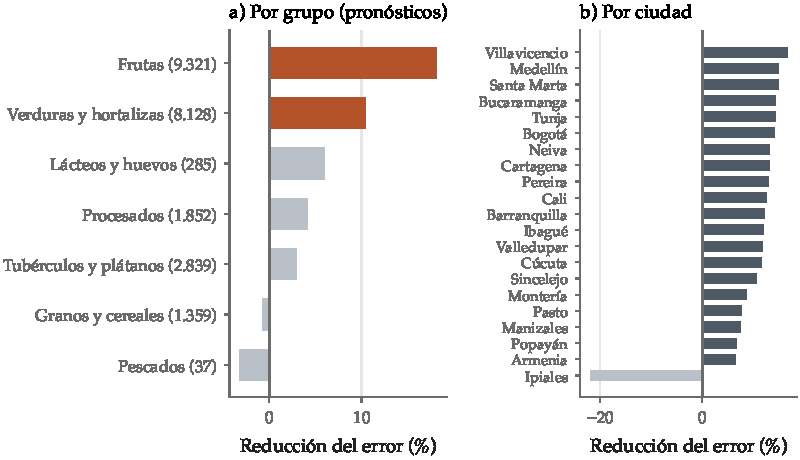
\includegraphics[width=.8\textwidth]{fig_grupos}
\caption{Reducción del error de CatBoost frente al último precio en la prueba, por grupo de alimentos (a; en naranja, los grupos con mejora significativa tras el ajuste de Holm) y por ciudad (b).}\label{fig:grupos}
\end{figure}

Entre los 20 productos con más pronósticos (figura~\ref{fig:productos}), las mayores reducciones se obtienen en remolacha (22\pct) y papa criolla (18\pct), productos con un patrón estacional marcado. En arroz, harinas y apio, el error de CatBoost supera en un 2--6\pct\ al del último precio, por razones distintas. En el arroz y las harinas el precio varía muy poco de un mes a otro (el MAE del último precio es inferior a 2 puntos), por lo que cualquier pronóstico distinto de cero tiende a aumentar el error. El apio, en cambio, es volátil, pero se movió mucho menos en la prueba que en el desarrollo: el MAE del último precio pasó de \rvapiodes\ a \rvapiorw\ puntos, y el modelo, estimado con la historia más volátil, pronosticó cambios que no ocurrieron (MAE de \rvapiocat).

\begin{figure}[htbp]\centering
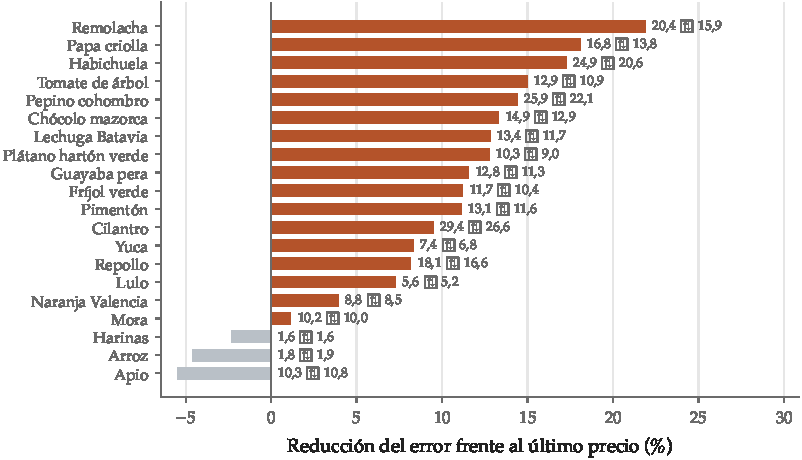
\includegraphics[width=.8\textwidth]{fig_productos}
\caption{Reducción del error de CatBoost frente al último precio en los 20 productos con más pronósticos de la prueba. A la derecha de cada barra, el MAE del último precio y el de CatBoost, en puntos porcentuales.}\label{fig:productos}
\end{figure}

A lo largo del periodo de prueba (figura~\ref{fig:mensual}a), CatBoost tuvo menor error que el último precio en 20 de los 21 meses. La mejora alcanzó el 26\pct\ en noviembre y diciembre de 2025 y fue pequeña entre mayo y septiembre de 2026 (entre $-6$\pct\ y 8\pct). La reducción mensual del error se correlaciona con el error del último precio en ese mes ($r=0{,}56$), es decir, la ganancia es mayor en los meses con más variación de precios.

La tabla~\ref{tab:reg_extra} presenta métricas que tratan las series por igual o que pesan más los errores grandes. El MASE y la media geométrica del MAE relativo por serie (AvgRelMAE de \rvavgrel\ para CatBoost, es decir, una reducción de cerca del 9\pct\ en la serie típica) conservan el orden de los modelos, y la RMSE de CatBoost (\rvrmsecat\ frente a \rvrmserw\ del último precio) indica que la mejora también se da en los cambios grandes. El promedio de XGBoost, LightGBM y CatBoost, definido de antemano y no elegido con la prueba, tiene un MAE de \rvensmae, prácticamente igual al de CatBoost (diferencia de \rvensdif\ puntos, intervalo \rvensdific).

\begin{table}[htbp]\centering\small
\caption{Métricas complementarias del pronóstico del cambio en la prueba: MAE y RMSE (puntos porcentuales), MASE (escala: MAE del último precio de cada serie en entrenamiento), media geométrica del MAE relativo al último precio por serie (AvgRelMAE; menor que 1 indica mejora en la serie típica), promedio simple de las reducciones del error por grupo (\%) y porcentaje de series en que el modelo tiene menor MAE que el último precio. $^\ast$Modelo elegido.}\label{tab:reg_extra}
\begin{adjustbox}{max width=\textwidth}\begin{tabular}{lrrrrrr}\toprule
Modelo & MAE & RMSE & MASE & AvgRelMAE & Red. media por grupo & Series que gana\\ \midrule
Paseo aleatorio & 12{,}06 & 18{,}40 & 0{,}940 & 1{,}000 & 0{,}0 & -- \\
AR estacional & 11{,}47 & 17{,}19 & 0{,}931 & 0{,}982 & 5{,}0 & 56 \\
SARIMA & 11{,}50 & 17{,}00 & 0{,}945 & 0{,}988 & \ensuremath{-}1{,}7 & 42 \\
\midrule
Regresión cuantílica & 11{,}07 & 16{,}29 & 0{,}938 & 0{,}974 & \ensuremath{-}3{,}6 & 63 \\
MLP & 10{,}67 & 15{,}71 & 0{,}867 & 0{,}918 & 3{,}9 & 72 \\
Random Forest & 10{,}69 & 15{,}88 & 0{,}872 & 0{,}918 & 5{,}3 & 73 \\
XGBoost & 10{,}60 & 15{,}60 & 0{,}873 & 0{,}921 & 4{,}5 & 71 \\
LightGBM & 10{,}59 & 15{,}64 & 0{,}859 & 0{,}912 & 5{,}7 & 73 \\
CatBoost$^\ast$ & 10{,}59 & 15{,}61 & 0{,}866 & 0{,}915 & 5{,}4 & 72 \\
\midrule
Promedio de XGBoost, LightGBM y CatBoost & 10{,}56 & -- & -- & -- & -- & -- \\
LightGBM cuantílico (mediana) & 10{,}60 & -- & -- & -- & -- & -- \\
\bottomrule\end{tabular}\end{adjustbox}\end{table}


\begin{figure}[htbp]\centering
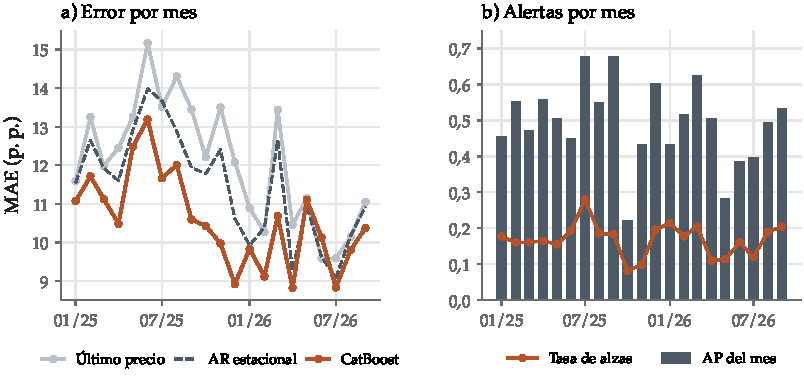
\includegraphics[width=.8\textwidth]{fig_mensual}
\caption{Resultados por mes de la prueba. (a) MAE del último precio, del AR estacional y de CatBoost. (b) AP mensual de CatBoost y tasa de alzas del mes; para un modelo sin información, la AP sería igual a la tasa.}\label{fig:mensual}
\end{figure}


\subsection{Análisis de los errores}

Los errores de CatBoost en la prueba están centrados, con una mediana de $-0{,}4$ puntos, y presentan colas pesadas, al igual que la variable objetivo (figura~\ref{fig:residuos}a). La autocorrelación mediana del error dentro de cada serie es de $-0{,}03$, lo que indica que no queda una estructura temporal simple sin aprovechar. En los extremos del pronóstico se observa un sesgo leve, ya que los cambios observados son algo menores que los pronosticados (figura~\ref{fig:residuos}b). Además, el error aumenta con la volatilidad pasada de la serie, desde unos 2 puntos en las series más estables hasta más de 20 en las más volátiles (figura~\ref{fig:residuos}c), lo que se refleja en intervalos de pronóstico más amplios para estas series (sección~\ref{sec:res_intervalos}).

\begin{figure}[htbp]\centering
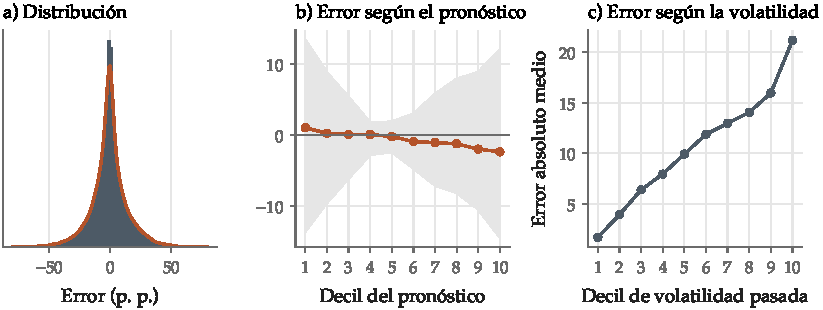
\includegraphics[width=.8\textwidth]{fig_residuos}
\caption{Errores de CatBoost en la prueba (observado menos pronosticado). (a) Distribución, recortada en $\pm80$ puntos. (b) Mediana y rango intercuartil del error por decil del pronóstico. (c) Error absoluto medio por decil de la volatilidad de los últimos doce meses.}\label{fig:residuos}
\end{figure}


\section{Resultados para las alzas mayores al 15\,\%}
\label{sec:res_clf}

\subsection{Balanceo de clases}

Ningún método de balanceo aumentó la AP de validación: en CatBoost fue de 0,524 sin balanceo, 0,521 con pesos y 0,521 con submuestreo, y en los demás modelos las diferencias fueron igual de pequeñas. De acuerdo con la proposición~\ref{prop:prior}, el submuestreo elevó la probabilidad media de 18\pct\ a cerca del 40\pct\ sin mejorar el ordenamiento de los casos. La corrección de las probabilidades con la muestra de validación fue mínima, ya que las probabilidades sin corregir estaban bien centradas.

\subsection{Comparación de los clasificadores y uso de las alertas}

CatBoost obtuvo la mayor AP en validación y fue el clasificador seleccionado. En la prueba alcanzó una AP de \cpre\ (intervalo de \cprloe\ a \cprhie), cerca de tres veces la tasa de alzas (\ctasaprueba\pct), y una AUC de \croce\ (tabla~\ref{tab:clf}). XGBoost obtuvo una AP algo mayor en la prueba (0,495), y la diferencia con CatBoost, de 0,014 (intervalo ajustado de 0,007 a 0,021), es significativa. Como el modelo se eligió por su AP de validación, donde CatBoost fue superior (0,524 frente a 0,520), la elección no se modifica con los resultados de la prueba; la diferencia equivale a menos del 3\pct\ de la AP. Los tres modelos de referencia tienen un desempeño inferior al de todos los modelos de aprendizaje automático y la diferencia con la frecuencia histórica es significativa, de modo que se acepta la hipótesis H2. La figura~\ref{fig:roc_pr} presenta las curvas ROC y de precisión y exhaustividad de todos los clasificadores.

\begin{table}[htbp]\centering\small
\caption{Anticipación de alzas mayores al 15\,\%. Área bajo la curva de precisión y exhaustividad (AP) en validación y en prueba, área bajo la curva ROC (AUC) en prueba, diferencia de AP con CatBoost (negativa: peor) y, con el umbral fijado en validación, precisión y exhaustividad en prueba (\%). Intervalos al 95\,\%; los de la diferencia, ajustados por comparaciones múltiples. $^\ast$Modelo elegido.}\label{tab:clf}
\begin{adjustbox}{max width=\textwidth}\begin{tabular}{lrrrrrr}\toprule
& \multicolumn{2}{c}{AP} & & Diferencia & & \\ \cmidrule(lr){2-3}
Modelo & Validación & Prueba & AUC & con CatBoost & Precisión & Exhaustividad\\ \midrule
Regresión logística & 0{,}502 & 0{,}465 [0{,}424; 0{,}501] & 0{,}804 & \ensuremath{-}0{,}016 [\ensuremath{-}0{,}045; 0{,}011] & 38 & 68 \\
MLP & 0{,}504 & 0{,}485 [0{,}441; 0{,}524] & 0{,}817 & 0{,}004 [\ensuremath{-}0{,}011; 0{,}018] & 39 & 64 \\
Random Forest & 0{,}521 & 0{,}490 [0{,}447; 0{,}533] & 0{,}820 & 0{,}009 [\ensuremath{-}0{,}008; 0{,}022] & 39 & 67 \\
XGBoost & 0{,}520 & 0{,}495 [0{,}454; 0{,}536] & 0{,}821 & 0{,}014 [0{,}007; 0{,}021] & 39 & 67 \\
LightGBM & 0{,}523 & 0{,}492 [0{,}448; 0{,}538] & 0{,}819 & 0{,}011 [\ensuremath{-}0{,}001; 0{,}022] & 39 & 69 \\
CatBoost$^\ast$ & 0{,}524 & 0{,}481 [0{,}439; 0{,}521] & 0{,}818 & -- & 37 & 71 \\
\midrule
SARIMA & -- & 0{,}431 [0{,}386; 0{,}469] & 0{,}789 & \ensuremath{-}0{,}049 [\ensuremath{-}0{,}087; \ensuremath{-}0{,}020] & -- & -- \\
Frecuencia histórica & -- & 0{,}396 [0{,}340; 0{,}451] & 0{,}766 & \ensuremath{-}0{,}085 [\ensuremath{-}0{,}126; \ensuremath{-}0{,}050] & -- & -- \\
Logística autorregresiva & -- & 0{,}381 [0{,}349; 0{,}414] & 0{,}727 & \ensuremath{-}0{,}100 [\ensuremath{-}0{,}129; \ensuremath{-}0{,}070] & -- & -- \\
\bottomrule\end{tabular}\end{adjustbox}\end{table}


\begin{figure}[htbp]\centering
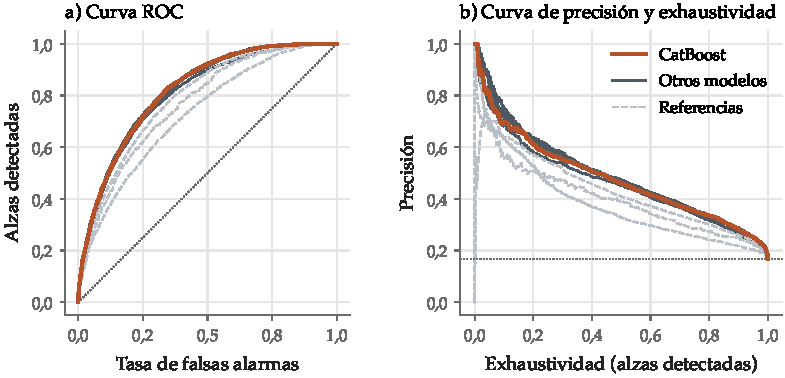
\includegraphics[width=.8\textwidth]{fig_roc_pr}
\caption{Curvas ROC (a) y de precisión y exhaustividad (b) de los nueve clasificadores en la prueba. La línea punteada indica un modelo sin información.}\label{fig:roc_pr}
\end{figure}

El umbral por defecto es el que maximiza $F_1$ en validación, $u=\cue$, que equivale a suponer que no alertar un alza cuesta unas \ccostoe\ veces lo que una falsa alarma ($c_{FP}:c_{FN}=0{,}22:0{,}78$). Este supuesto es cercano a la razón 1:3 ($u=0{,}25$) que se usa como ejemplo en el resto del capítulo, y los resultados con otros umbrales están en la tabla~\ref{tab:alertas}. Con $u=\cue$, CatBoost emite alertas en el \calertase\pct\ de los casos, detecta el \crece\pct\ de las alzas y acierta en el \cprece\pct\ de sus alertas (\cvp\ alzas detectadas, \cfp\ falsas alarmas y \cfn\ alzas no detectadas). Las alzas detectadas corresponden principalmente a verduras (\crecver\pct) y frutas (\crecfru\pct), y en tubérculos la tasa de detección es del \crectub\pct. En los demás grupos se registraron solo \calzasotros\ alzas en todo el periodo, y ninguna fue detectada.


Las probabilidades están bien ordenadas y cercanas a la diagonal (figura~\ref{fig:calibracion}a), aunque sobrestiman ligeramente el riesgo, con una probabilidad media de \cprobmedia\pct\ frente a una tasa observada de \ctasaprueba\pct. Esta diferencia coincide con la disminución de la tasa de alzas entre la validación (\ctasaval\pct) y la prueba, que no podía anticiparse con información anterior a 2025. La tabla~\ref{tab:clf_extra} complementa el gráfico con reglas de puntuación propias. CatBoost tiene un puntaje de Brier de \rvbrier, frente a \rvbrierfh\ de la frecuencia histórica, lo que da un \emph{Brier skill score} del \rvbss\pct\ (intervalo \rvbssic). Su pendiente de calibración es \rvpend\ (intervalo \rvpendic), compatible con 1, y su intercepto, \rvintercal, refleja la leve sobrestimación del riesgo. El SARIMA, en cambio, tiene una pendiente de \rvpendsar: sus probabilidades son demasiado extremas.

\begin{table}[htbp]\centering\small
\caption{Reglas de puntuación propias y calibración de las probabilidades en la prueba: puntaje de Brier, \emph{Brier skill score} frente a la frecuencia histórica (BSS, \%), pérdida logarítmica, intercepto (con pendiente fija en 1) y pendiente de calibración, y error esperado de calibración por deciles (ECE, puntos porcentuales). Entre corchetes, intervalos bootstrap por bloques de meses al 95\,\%. $^\ast$Modelo elegido.}\label{tab:clf_extra}
\begin{adjustbox}{max width=\textwidth}\begin{tabular}{lrrrrrr}\toprule
Modelo & Brier & BSS (\%) & Log-loss & Intercepto & Pendiente & ECE\\ \midrule
Regresión logística & 0{,}1142 [0{,}1025; 0{,}1237] & 6{,}0 [4{,}5; 8{,}5] & 0{,}367 & \ensuremath{-}0{,}12 & 1{,}08 [1{,}00; 1{,}19] & 2{,}0 \\
MLP & 0{,}1125 [0{,}1015; 0{,}1201] & 7{,}3 [5{,}3; 10{,}2] & 0{,}356 & \ensuremath{-}0{,}20 & 0{,}95 [0{,}90; 1{,}02] & 2{,}3 \\
Random Forest & 0{,}1114 [0{,}1008; 0{,}1191] & 8{,}3 [7{,}0; 10{,}4] & 0{,}353 & \ensuremath{-}0{,}16 & 1{,}06 [0{,}99; 1{,}15] & 1{,}9 \\
XGBoost & 0{,}1114 [0{,}1002; 0{,}1194] & 8{,}3 [6{,}4; 11{,}1] & 0{,}353 & \ensuremath{-}0{,}20 & 1{,}00 [0{,}94; 1{,}08] & 2{,}3 \\
LightGBM & 0{,}1120 [0{,}1010; 0{,}1197] & 7{,}8 [5{,}6; 10{,}8] & 0{,}355 & \ensuremath{-}0{,}21 & 0{,}99 [0{,}92; 1{,}07] & 2{,}5 \\
CatBoost$^\ast$ & 0{,}1123 [0{,}1010; 0{,}1206] & 7{,}5 [5{,}9; 10{,}0] & 0{,}356 & \ensuremath{-}0{,}18 & 1{,}00 [0{,}93; 1{,}10] & 2{,}1 \\
\midrule
SARIMA & 0{,}1208 [0{,}1113; 0{,}1290] & 0{,}5 [\ensuremath{-}1{,}9; 2{,}7] & 0{,}395 & \ensuremath{-}0{,}27 & 0{,}65 [0{,}60; 0{,}70] & 3{,}4 \\
Frecuencia histórica & 0{,}1215 [0{,}1110; 0{,}1303] & -- & 0{,}387 & \ensuremath{-}0{,}07 & 0{,}87 [0{,}82; 0{,}94] & 1{,}9 \\
Logística autorregresiva & 0{,}1251 [0{,}1122; 0{,}1358] & \ensuremath{-}3{,}0 [\ensuremath{-}4{,}9; \ensuremath{-}0{,}5] & 0{,}403 & \ensuremath{-}0{,}17 & 0{,}96 [0{,}89; 1{,}08] & 2{,}3 \\
\bottomrule\end{tabular}\end{adjustbox}\end{table}


La tabla~\ref{tab:alertas} presenta el uso de las alertas con distintos umbrales. En la prueba hay en promedio 1\,134 pronósticos y 191 alzas por mes. Si una falsa alarma tiene el mismo costo que un alza no alertada ($u=0{,}5$), el modelo emite unas 96 alertas mensuales, con una precisión del 56\pct\ y una exhaustividad del 28\pct. Si el costo de no alertar un alza es tres veces mayor ($u=0{,}25$), se emiten unas 312 alertas, con una precisión del 40\pct\ y una exhaustividad cercana a dos tercios.

\begin{table}[htbp]\centering\small
\caption{Alertas de CatBoost en la prueba según la razón de costos entre una falsa alarma y un alza no alertada. Umbral $u=c_{FP}/(c_{FP}+c_{FN})$; alertas promedio por mes (de unos 1134 pronósticos mensuales, con 191 alzas en promedio); porcentaje de casos alertados; precisión y exhaustividad (\%), y beneficio neto (alzas netas por cada 100 casos)}\label{tab:alertas}
\begin{adjustbox}{max width=\textwidth}\begin{tabular}{lrrrrrr}\toprule
Razón $c_{FP}:c_{FN}$ & Umbral & Alertas al mes & Casos alertados & Precisión & Exhaustividad & Beneficio neto\\ \midrule
1:1 & 0{,}50 & 96 & 8{,}5 & 56{,}2 & 28{,}4 & 1{,}05 \\
1:2 & 0{,}33 & 217 & 19{,}2 & 45{,}3 & 51{,}6 & 3{,}45 \\
1:3 & 0{,}25 & 312 & 27{,}5 & 39{,}7 & 64{,}9 & 5{,}40 \\
1:5 & 0{,}17 & 464 & 40{,}9 & 33{,}2 & 80{,}7 & 8{,}11 \\
1:9 & 0{,}10 & 644 & 56{,}8 & 27{,}2 & 91{,}9 & 10{,}86 \\
\bottomrule\end{tabular}\end{adjustbox}\end{table}


La AP mensual varía entre \cprmeslo\ y \cprmeshi\ (figura~\ref{fig:mensual}b), en parte porque tiende a aumentar con la tasa de alzas del mes. La AUC mensual, que no depende de esa tasa, varía entre \crocmeslo\ y \crocmeshi\ y tiene una correlación baja con ella ($r=\ccorrroc$).

El beneficio neto de CatBoost es superior al de alertar siempre, al de no alertar y al de la frecuencia histórica en todo el rango de umbrales evaluado, entre 0,05 y 0,60 (figura~\ref{fig:calibracion}b), lo que confirma la hipótesis H3. Con $u=0{,}25$, el modelo obtiene \cbnvc\ alzas netas por cada 100 casos, \cbndfrec\ más que la frecuencia histórica.

\begin{figure}[htbp]\centering
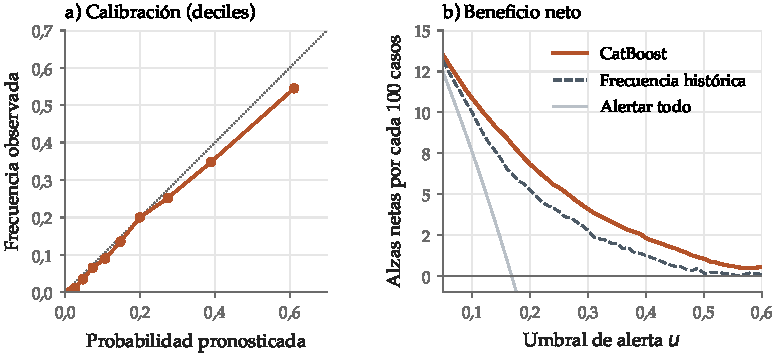
\includegraphics[width=.8\textwidth]{fig_calibracion}
\caption{CatBoost en la prueba. (a) Frecuencia observada de alzas frente a la probabilidad pronosticada, por deciles; la diagonal indica calibración perfecta. (b) Beneficio neto según el umbral de alerta.}\label{fig:calibracion}
\end{figure}


\subsection{Dos series de ejemplo}
\label{sec:res_caso}

La figura~\ref{fig:caso} presenta dos series con resultados contrastantes. Se eligieron entre los cuatro productos más volátiles del panel (tabla~\ref{tab:volatiles}), antes de mirar sus resultados en la prueba, para ilustrar una serie con estacionalidad marcada y otra sin patrón: el cilantro en su central de mayor volumen (Corabastos) y el mango Tommy en la Central Mayorista de Antioquia, que es la serie de ejemplo del SARIMA y de la descomposición STL. El precio del mango Tommy en la Central Mayorista de Antioquia tiene un ciclo estacional marcado, que el pronóstico de CatBoost reproduce de cerca; el error pasa de 35,2 puntos con el último precio a 19,6 con el modelo. De las 13 alertas emitidas, 11 correspondieron a alzas, y el intervalo del 80\pct\ contuvo el valor observado en 19 de los 21 meses.

El precio del cilantro en Corabastos presenta cambios superiores al 50\pct\ en ambas direcciones y sin un patrón regular. En esta serie el pronóstico se mantiene cerca de cero y la reducción del error es pequeña (de 53,5 a 50,7 puntos). El modelo emitió alertas en 18 de los 21 meses y detectó las 10 alzas, con 8 falsas alarmas. El intervalo del 80\pct\ tuvo un ancho promedio cercano a 100 puntos y contuvo el valor observado solo en 11 meses (52\pct). La garantía de la calibración conforme es marginal, es decir, se cumple en promedio sobre todas las series, y puede ocultar subcobertura en las más volátiles; la sección~\ref{sec:res_intervalos} lo examina por decil de volatilidad.

\begin{figure}[htbp]\centering
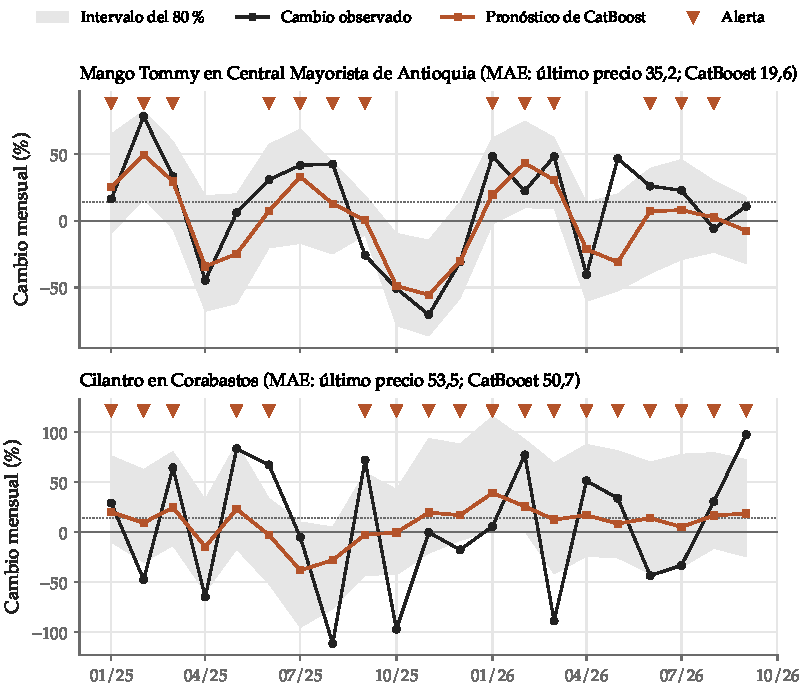
\includegraphics[width=.8\textwidth]{fig_caso}
\caption{Cambio mensual observado, pronóstico de CatBoost e intervalo conforme del 80\pct\ en dos series de la prueba. Los triángulos marcan los meses con alerta ($u=\cue$) y la línea punteada el umbral de alza del 15\pct.}\label{fig:caso}
\end{figure}


\section{Comparación estadística entre modelos}
\label{sec:comparacion}

La prueba de Friedman compara simultáneamente todos los modelos a partir de su ordenamiento en cada uno de los 21 meses. En regresión se rechaza la hipótesis de igualdad ($\chi^2_F=98{,}7$, $p<0{,}001$). De acuerdo con la prueba de Nemenyi, con una diferencia crítica de 2,62 entre rangos medios, los cinco modelos no lineales forman un grupo sin diferencias significativas, con rangos medios entre 2,95 y 3,76, separado de la regresión cuantílica, los modelos de referencia y el último precio.

En clasificación también se rechaza la hipótesis de igualdad ($\chi^2_F=81{,}4$, $p<0{,}001$). XGBoost obtiene el mejor rango medio (2,62, frente a 3,90 de CatBoost), y nuevamente los modelos no lineales no presentan diferencias significativas entre sí. Con 21 meses la potencia de la prueba es limitada; por ejemplo, CatBoost no se distingue estadísticamente del SARIMA, aunque tiene mayor AP en 18 de los 21 meses. Además, la prueba supone meses independientes, lo que no se cumple, de modo que sus valores $p$ son aproximados y se usa como complemento de los intervalos bootstrap por bloques.


La prueba de DeLong encuentra diferencias de AUC pequeñas entre CatBoost y los demás clasificadores de aprendizaje automático, de 0,001 a 0,014 en valor absoluto, significativas solo frente a XGBoost y a la regresión logística, y diferencias mayores frente a las referencias, de 0,029 a 0,091. Esta prueba supone independencia entre los pronósticos, supuesto que no se cumple para los pronósticos de un mismo mes. Por esta razón se da prioridad a los intervalos bootstrap por meses de la tabla~\ref{tab:clf}, según los cuales, entre los modelos no lineales, solo XGBoost supera a CatBoost, por un margen pequeño.

\section{Interpretabilidad}
\label{sec:res_importancia}

Al permutar los bloques de variables en la prueba, la historia del precio es el bloque con mayor efecto sobre el desempeño, con un aumento del MAE de \cibrhist\ puntos y una disminución de la AP de \cibchist, en promedio de diez permutaciones. Le siguen la estacionalidad (\cibrest\ puntos y \cibcest) y, en menor medida, la red de centrales y el bloque de producto y lugar. El abastecimiento nacional tiene un efecto pequeño (0,05 puntos de MAE y ninguno en la AP). Estas medidas reflejan cuánto depende el modelo de cada bloque y no un efecto causal.


Para conocer la dirección del efecto de cada variable se calcularon los valores de Shapley de todos los pronósticos de la prueba (sección~\ref{sec:shap}). Los programas guardan los modelos finales al estimarlos, y los valores de Shapley se calcularon sobre esos objetos guardados; al cargarlos, ambos reproducen exactamente los pronósticos evaluados (apéndice~\ref{ap:reproduccion}).

En la figura~\ref{fig:shap} cada punto corresponde a un pronóstico; la posición horizontal indica el aporte de la variable al pronóstico y el color, si su valor era alto o bajo. En el modelo de regresión, las tres variables con mayor aporte son las siguientes:
\begin{itemize}[nosep]
\item \emph{Cambio histórico en el mes} (11\pct\ del aporte total). Si el precio de la serie tendía a subir en ese mes en años anteriores, el pronóstico es mayor.
\item \emph{Cambio en las demás centrales} (11\pct). Un aumento del precio del producto en otras centrales se asocia con un pronóstico de aumento en la central, lo que es consistente con la transmisión de precios con rezago.
\item \emph{Distancia al mínimo anual} (10\pct). Cuando el precio está muy por encima de su mínimo del último año, el pronóstico es de disminución.
\end{itemize}
En el modelo de clasificación la variable con mayor aporte es la distancia al máximo anual (14\pct): un precio muy inferior a su máximo se asocia con un mayor riesgo de alza. Le siguen la frecuencia histórica de alzas en el mes, el cambio en las demás centrales y el cambio histórico en el mes. Las variables de abastecimiento nacional suman el 5\pct\ del aporte en regresión y el 6\pct\ en clasificación, y los códigos de central y ciudad tienen un aporte inferior al 0,3\pct, lo que indica que el modelo no depende de la identidad del lugar. Los nombres de las variables en las figuras son los mismos de la tabla~\ref{tab:variables}.

\begin{figure}[htbp]\centering
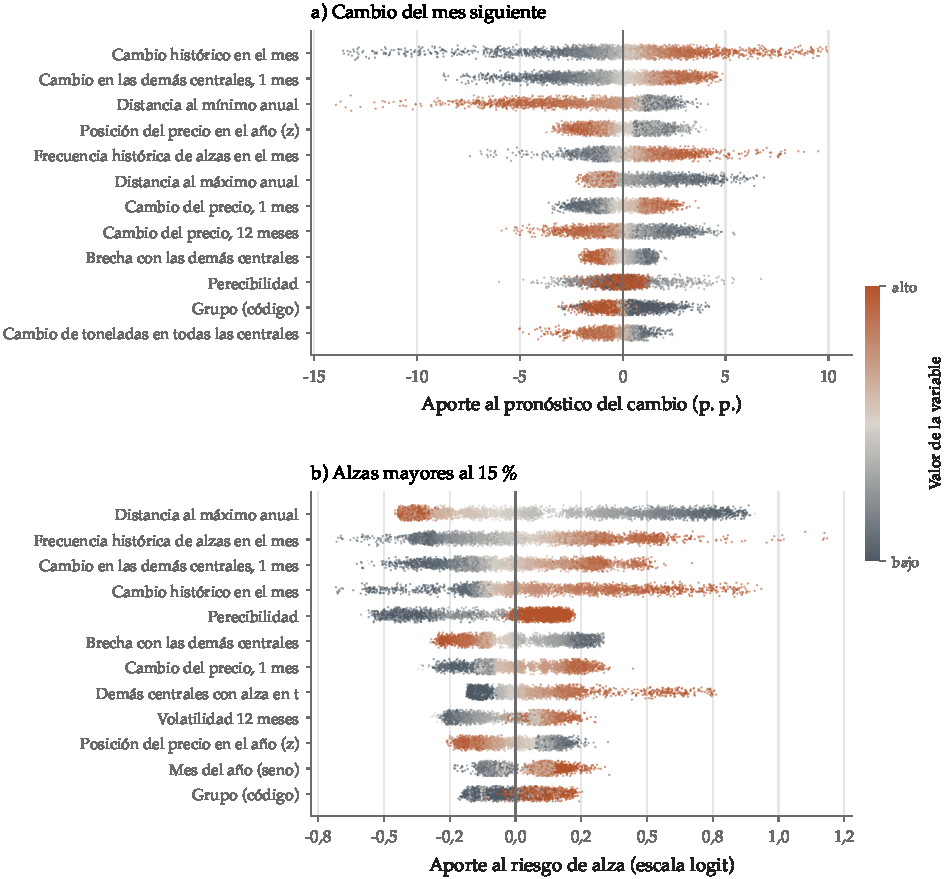
\includegraphics[width=.8\textwidth]{fig_shap}
\caption{Valores de Shapley de CatBoost en la prueba (muestra de 6\,000 pronósticos) para las doce variables con mayor aporte medio. Cada punto es un pronóstico; el color indica el valor de la variable dentro de su rango.}\label{fig:shap}
\end{figure}

Los valores de Shapley también permiten descomponer pronósticos individuales (figura~\ref{fig:shap_casos}). En febrero de 2025, la probabilidad de alza del mango Tommy en Medellín pasó del 12\pct\ al 93\pct. El punto de partida es $\phi_0$, el promedio del logit del modelo; su transformación (12\pct) es menor que la probabilidad media pronosticada (18,9\pct) porque la función logística no es lineal. Los principales aportes provinieron de su comportamiento histórico en febrero (aumento promedio cercano al 60\pct\ y alzas fuertes en tres de cada cuatro años) y de que el precio estaba un \rvmangomax\pct\ por debajo de su máximo anual. El precio aumentó un 118\pct.

En el caso del cilantro en la central de Manizales en mayo de 2025, la probabilidad asignada fue del 7\pct. El precio había caído un 21\pct\ en el mes anterior, el mismo producto había bajado un 24\pct\ en las demás centrales y en mayo esta serie había registrado disminuciones en cinco de los seis años anteriores. Sin embargo, el precio aumentó un 85\pct. Este tipo de cambios de dirección sin señales previas en los precios concentra los errores más costosos del modelo.

\begin{figure}[htbp]\centering
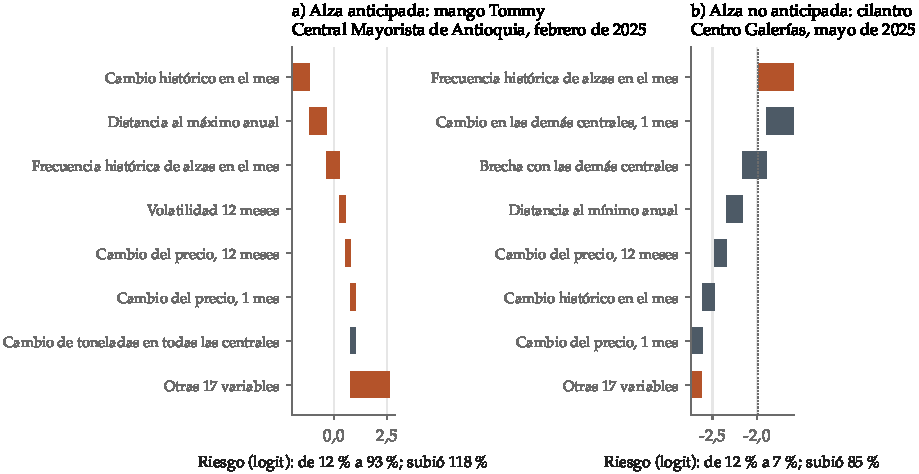
\includegraphics[width=.8\textwidth]{fig_shap_casos}
\caption{Aportes de las variables al riesgo de alza en dos pronósticos de la prueba, en escala logit. Las barras parten del riesgo promedio del modelo y se acumulan hasta el pronóstico final; naranja sube el riesgo y gris lo baja.}\label{fig:shap_casos}
\end{figure}


\section{Intervalos de pronóstico}
\label{sec:res_intervalos}

Se estimaron siete cuantiles del cambio, $\tau\in\{0{,}05;0{,}10;0{,}25;0{,}50;0{,}75;0{,}90;0{,}95\}$, con un LightGBM por cuantil y pérdida de pinball. Sus hiperparámetros, comunes a los siete, se eligieron con la misma búsqueda y los mismos tres años de validación que los demás modelos, minimizando la pinball promedio. Los cuantiles estimados se cruzaron en el \rvcruces\pct\ de los casos; se ordenaron de menor a mayor, lo que equivale al reordenamiento de \citet{chernozhukov2010}. La probabilidad de alza se obtiene interpolando linealmente $\hat F(c\mid\mathbf{x})$ entre los cuantiles, con colas en 0,025 y 0,975. Para la calibración conforme, los modelos se estimaron con datos hasta 2023, se calibraron con los 12 meses de 2024 y se aplicaron sin cambios a la prueba, de modo que la muestra de calibración termina justo antes de la prueba y no se usa para estimar. La mediana del modelo de cuantiles estimado con 2019--2024 tiene un MAE de \rvqmae\ en la prueba, una reducción del \rvqred\pct\ frente al último precio, casi igual a la de CatBoost.

Los intervalos del 90\pct\ contienen el valor observado en el \ccobnovq\pct\ de los casos de la prueba, con una cobertura menor en los perecederos (\ccobnovqper\pct; tabla~\ref{tab:cqr}). La calibración conforme global corrige esta subcobertura, pero sobrecubre a los no perecederos (\ccobnovcgnoper\pct). La calibración por grupo deja ambos grupos cerca del 90\pct, con intervalos un 7\pct\ más anchos. La probabilidad de alza obtenida a partir de los mismos cuantiles tiene un desempeño similar al del clasificador (AP de \cdqpr\ frente a \cpre).

\begin{table}[htbp]\centering\small
\caption{Intervalos de pronóstico en prueba: porcentaje de casos cuyo cambio observado cae dentro del intervalo (cobertura) y ancho medio en puntos porcentuales. Perecederos: frutas, verduras y tubérculos.}\label{tab:cqr}
\begin{adjustbox}{max width=\textwidth}\begin{tabular}{lrrrrrr}\toprule
& \multicolumn{4}{c}{Intervalo del 90\,\%} & \multicolumn{2}{c}{Intervalo del 80\,\%}\\ \cmidrule(lr){2-5}\cmidrule(lr){6-7}
Método & Cobertura & Perecederos & No perec. & Ancho & Cobertura & Ancho\\ \midrule
Cuantiles estimados & 88{,}9 & 88{,}8 & 89{,}8 & 43{,}6 & 79{,}8 & 33{,}4 \\
Conforme, global & 91{,}0 & 90{,}4 & 94{,}3 & 45{,}8 & 81{,}0 & 34{,}3 \\
Conforme, por grupo & 91{,}1 & 91{,}1 & 91{,}5 & 46{,}5 & 81{,}2 & 34{,}8 \\
\bottomrule\end{tabular}\end{adjustbox}\end{table}


La cobertura promedio oculta diferencias entre series (tabla~\ref{tab:cobertura}). Con la calibración por grupo, el intervalo del 90\pct\ cubre el \rvcobdecuno\pct\ de los casos en el decil de series más estables y el \rvcobdecdiez\pct\ en el más volátil, con anchos de \rvanchdecuno\ y \rvanchdecdiez\ puntos. Es decir, la calibración conforme por grupo garantiza la cobertura marginal, pero no la condicional: los intervalos son demasiado anchos en las series estables y algo angostos en las más volátiles. Una calibración por decil de volatilidad, en lugar de por grupo de alimentos, corregiría parte de esa diferencia.

\begin{table}[htbp]\centering\small
\caption{Cobertura condicional de los intervalos en la prueba por decil de volatilidad de los últimos doce meses (1 = series más estables): volatilidad media (p.~p.), cobertura (\%) de los cuantiles estimados y de la calibración conforme por grupo, y ancho medio del intervalo conforme del 90\,\% (p.~p.). La última fila da el puntaje de intervalo de \citet{gneiting2007} (menor es mejor).}\label{tab:cobertura}
\begin{adjustbox}{max width=\textwidth}\begin{tabular}{lrrrrrr}\toprule
& & \multicolumn{3}{c}{Intervalo del 90\,\%} & \multicolumn{2}{c}{Intervalo del 80\,\%}\\ \cmidrule(lr){3-5}\cmidrule(lr){6-7}
Decil & Volatilidad & Cuantiles & Conforme & Ancho & Cuantiles & Conforme\\ \midrule
1 & 1{,}8 & 92{,}5 & 93{,}6 & 10{,}6 & 85{,}4 & 84{,}9 \\
2 & 4{,}8 & 90{,}1 & 92{,}2 & 20{,}2 & 80{,}8 & 83{,}0 \\
3 & 7{,}9 & 90{,}5 & 92{,}6 & 31{,}1 & 80{,}8 & 83{,}2 \\
4 & 10{,}7 & 90{,}7 & 93{,}2 & 39{,}0 & 81{,}5 & 84{,}0 \\
5 & 13{,}4 & 89{,}7 & 92{,}4 & 46{,}2 & 80{,}7 & 82{,}6 \\
6 & 16{,}2 & 88{,}1 & 90{,}1 & 51{,}7 & 78{,}3 & 80{,}6 \\
7 & 19{,}4 & 87{,}3 & 89{,}2 & 56{,}0 & 76{,}3 & 78{,}1 \\
8 & 23{,}1 & 88{,}1 & 90{,}2 & 60{,}4 & 77{,}9 & 79{,}2 \\
9 & 28{,}6 & 88{,}3 & 90{,}1 & 67{,}7 & 78{,}4 & 79{,}3 \\
10 & 40{,}9 & 86{,}0 & 87{,}9 & 82{,}6 & 76{,}2 & 77{,}3 \\
\midrule Todos & -- & 89{,}1 & 91{,}1 & 46{,}5 & 79{,}6 & 81{,}2 \\
Puntaje de intervalo & -- & 59{,}7 & 59{,}7 & -- & 49{,}6 & 49{,}6 \\
\bottomrule\end{tabular}\end{adjustbox}\end{table}



\section{Robustez}
\label{sec:res_robustez}

La tabla~\ref{tab:robustez} resume los análisis de sensibilidad. Con bloques de uno a seis meses en el bootstrap, el límite inferior del intervalo de la mejora de CatBoost varía entre \csenslo\pct\ y \csenshi\pct. La reestimación trimestral de los modelos durante la prueba redujo levemente el error del pronóstico del cambio (\commovil\ frente a \comfijo; diferencia de \comd\ puntos, intervalo de \comdlo\ a \comdhi) y aumentó la AP de \comprf\ a \comprm, una diferencia no significativa. En cuanto a los faltantes, el precio del mes siguiente no está disponible en el \cfatasa\pct\ de los casos (\cfatasap\pct\ en la prueba); incluso si todos ellos fueran alzas, la AP disminuiría solo de \cfapro\ a \cfaprt. Al valorar el error en pesos, como la diferencia absoluta entre el precio pronosticado y el observado multiplicada por las toneladas del mes, CatBoost reduce el error del último precio en un \cvale\pct; las series sin registro de abastecimiento quedan con peso cero. En los escenarios de faltantes, \emph{todos alzas} imputa un cambio de $\ln 1{,}3$ (una subida del 30\pct) y \emph{ninguna alza} usa el cambio de las demás centrales con la indicadora de alza en cero.

El efecto de promediar precios (sección~\ref{sec:economia}) se evaluó de dos formas. Primero, con una referencia que lo incorpora, $\hat y=0{,}25\,r_t$, que pronostica el cambio que implicaría un paseo aleatorio en el precio puntual: su error es un \rvwkarabs\pct\ mayor que el del último precio, y CatBoost la supera en un \rvwkcat\pct\ (intervalo \rvwkcatic). Segundo, con un pronóstico a dos meses, que también responde al rezago de publicación (sección~\ref{sec:fuga}): con la información del mes $t$ se pronostica el cambio entre $t+1$ y $t+2$, un horizonte completo que empieza después de publicado el boletín y que no se ve afectado por la correlación que induce el promedio. Con los mismos hiperparámetros de CatBoost y las variables estacionales del mes $t+2$, el error se reduce en un \rvhdosred\pct\ frente al último precio (intervalo \rvhdosredic), con mejoras del \rvhdosfru\pct\ en frutas y del \rvhdosver\pct\ en verduras. La AP para las alzas de $t+2$ es \rvhdosap\ (intervalo \rvhdosapic), frente a \rvhdosfrec\ de la frecuencia histórica (diferencia de \rvhdosdif, intervalo \rvhdosdific). La capacidad de pronóstico disminuye con el horizonte, pero no desaparece, de modo que no se debe solo al efecto del promedio ni a la parte del mes ya transcurrida al publicarse el boletín.

La comparación de familias de modelos podría depender de dos decisiones que favorecen a los árboles: la codificación de las variables categóricas y la selección de variables con LightGBM. La tabla~\ref{tab:lineales} reestima la regresión cuantílica, la regresión logística y la red neuronal con indicadores de producto, central y ciudad y con las 52 candidatas. Con indicadores, la regresión cuantílica reduce el error en un \rvlinoh\pct\ y la red en un \rvmlpoh\pct; con las 52 candidatas, la regresión cuantílica llega al \rvlincand\pct. Ninguna de las dos decisiones explica, por tanto, la ventaja de los modelos no lineales. En cambio, una regresión cuantílica con interacciones entre el grupo y cada variable llega al \rvlininter\pct\ (AP de \rvlininterap\ en su versión logística), lo que indica que buena parte de esa ventaja proviene de permitir que el efecto de las variables cambie según el tipo de producto.

\begin{table}[htbp]\centering\small
\caption{Robustez de los resultados principales: reducción del error de CatBoost frente al último precio (\%) y AP de CatBoost en la prueba bajo cada variante; entre corchetes, intervalos del 95\,\%}\label{tab:robustez}
\begin{adjustbox}{max width=\textwidth}\begin{tabular}{lrr}\toprule
Variante & Reducción del error (\%) & AP\\ \midrule
Resultado principal & 12{,}2 [8{,}3; 16{,}9] & 0{,}481 [0{,}439; 0{,}521] \\
Bloques de 1 mes en el bootstrap & [8{,}9; 15{,}5] & [0{,}439; 0{,}523] \\
Bloques de 6 meses en el bootstrap & [9{,}4; 18{,}2] & [0{,}459; 0{,}522] \\
Reajuste trimestral & 12{,}6 & 0{,}484 \\
Faltantes: cambio de las demás centrales & 12{,}2 & 0{,}481 \\
Faltantes: todos alzas & 12{,}1 & 0{,}472 \\
Faltantes: ninguna alza & 12{,}2 & 0{,}475 \\
Error valorado en pesos & 11{,}7 [7{,}6; 17{,}6] & -- \\
\midrule
Bootstrap estacionario ($B=10\,000$) & [7{,}6; 16{,}6] & -- \\
Frente a la referencia $\hat y=0{,}25\,r_t$ (Working) & 13{,}2 [10{,}2; 17{,}0] & -- \\
Promedio de XGBoost, LightGBM y CatBoost & 12{,}5 [8{,}5; 17{,}0] & 0{,}493 [0{,}452; 0{,}536] \\
Cambio de $t+1$ a $t+2$ con información de $t$ & 8{,}8 [4{,}5; 14{,}4] & 0{,}464 [0{,}423; 0{,}517] \\
\bottomrule\end{tabular}\end{adjustbox}\end{table}


\begin{table}[htbp]\centering\small
\caption{Robustez de los modelos lineales y de la red neuronal en la prueba, con los hiperparámetros elegidos en validación: reducción del error frente al último precio (\%) y AP. Las variables categóricas entran como indicadores (\emph{one-hot}); las numéricas, estandarizadas con los datos de ajuste.}\label{tab:lineales}
\begin{adjustbox}{max width=\textwidth}\begin{tabular}{lrrrrr}\toprule
& & \multicolumn{2}{c}{Reducción del error (\%)} & \multicolumn{2}{c}{AP}\\ \cmidrule(lr){3-4}\cmidrule(lr){5-6}
Especificación & Columnas & Reg. cuantílica & MLP & Reg. logística & MLP\\ \midrule
Indicadores de grupo, 24 variables (original) & 32 & 8{,}2 & 11{,}5 & 0{,}465 & 0{,}485 \\
Indicadores de grupo, producto, central y ciudad; 24 variables & 184 & 7{,}8 & 10{,}5 & 0{,}465 & 0{,}493 \\
Indicadores de grupo, producto, central y ciudad; 52 candidatas & 207 & 7{,}4 & 11{,}1 & 0{,}462 & 0{,}479 \\
Interacciones grupo × variables; 24 variables & 359 & 10{,}2 & -- & 0{,}480 & -- \\
\midrule
Referencia: CatBoost y CatBoost & -- & \multicolumn{2}{c}{12{,}2} & \multicolumn{2}{c}{0{,}481} \\
\bottomrule\end{tabular}\end{adjustbox}\end{table}


Las tres implementaciones propias superaron la verificación descrita en el apéndice~\ref{ap:modelos}. El bosque de LightGBM presenta un error 0,19 puntos mayor que el Random Forest de scikit-learn en la submuestra de verificación, por lo que el desempeño del Random Forest reportado en este trabajo podría ser ligeramente inferior al del algoritmo original.

\section{Costo computacional y reproducibilidad}
\label{sec:res_costo}

El estudio completo se ejecutó en cerca de dos horas en un computador portátil con chip Apple de 10 núcleos y un uso máximo de memoria de \cmemmax\,GB. Los pasos de la tabla~\ref{tab:tiempos} tomaron \ctiempototal\ minutos y los análisis complementarios, las figuras y las tablas, unos 10 minutos más. Los pasos de mayor duración fueron la búsqueda de hiperparámetros de los clasificadores (28 minutos), la estimación de los SARIMA (20 minutos), las métricas con 10\,000 réplicas bootstrap (18 minutos) y los análisis complementarios (18 minutos).

La tabla~\ref{tab:costo} del apéndice compara la complejidad teórica de cada modelo con el tiempo de su búsqueda. Los modelos de potenciación escalan linealmente con el número de observaciones y de variables, ya que buscan los puntos de corte sobre histogramas, y su búsqueda tomó entre uno y tres minutos. El modelo más costoso fue el Random Forest de clasificación, con unos 17 minutos, debido a que la implementación de scikit-learn ordena los datos en cada división y los árboles son profundos.

Las configuraciones de cada búsqueda se evaluaron en paralelo, una por núcleo y con un hilo por modelo. El código está organizado en programas numerados que guardan sus resultados en archivos, a partir de los cuales se generan las tablas y figuras del documento. Las versiones de las librerías y las semillas aleatorias están fijadas (apéndice~\ref{ap:reproduccion}).

\section{Conclusiones del modelado con aprendizaje automático}
\label{sec:conclusiones_ml}

Los modelos de aprendizaje automático superaron a los modelos de referencia. CatBoost redujo el error del último precio en un \cmeje\pct\ y obtuvo un error significativamente menor que el AR estacional y el SARIMA, resultado que se mantuvo por mes, por ciudad, con reestimación trimestral y con el error ponderado por toneladas. Los cuatro modelos de árboles fueron estadísticamente equivalentes y la red neuronal quedó ligeramente por detrás. Su ventaja sobre el modelo lineal aditivo no se debe a la codificación de las variables categóricas ni a la selección de variables, y se reduce cuando el modelo lineal incluye interacciones entre el grupo de alimentos y las variables. La capacidad de pronóstico se mantiene, aunque menor, a dos meses. La mejora se concentró en frutas y verduras, mientras que en granos y procesados el último precio sigue siendo un pronóstico difícil de superar.

En cuanto a las alzas, el modelo detectó cerca de siete de cada diez con una precisión del \cprece\pct; en la prueba, XGBoost obtuvo una AP ligeramente mayor, aunque CatBoost había sido superior en validación. El beneficio neto del modelo seleccionado fue superior al de alertar siempre o nunca en todo el rango de costos evaluado. El balanceo de clases no mejoró los resultados y las probabilidades sin balancear presentaron una buena calibración. El análisis de los valores de Shapley indica que el modelo se apoya en la transmisión de precios entre centrales, la estacionalidad de cada serie y la tendencia de los precios extremos a corregirse, y que sus mayores errores corresponden a cambios de dirección sin señales previas en los precios.

\FloatBarrier

\chapter{Discusión}
\label{cap:discusion}

En este capítulo se discuten los resultados de cada objetivo específico en relación con la literatura.


\section{Objetivo 1: análisis exploratorio}

Los perecederos presentan cambios grandes y alzas frecuentes, mientras que los granos y procesados casi no varían, lo que es consistente con la teoría del almacenamiento \citep{working1949,deaton1992}. La selección de variables confirmó lo que anticipó el análisis exploratorio: ninguna variable sola se relaciona fuertemente con el cambio, y el abastecimiento local y el ONI no aportan.

\section{Objetivo 2: modelo clásico}

Los resultados del SARIMA por año muestran que una validación con un solo año habría conducido a conclusiones distintas: en 2022 el SARIMA fue un \rvsaraabs\pct\ peor que el último precio, mientras que en 2023 y 2024 fue mejor. La ausencia de autocorrelación en los residuos de la mayoría de las series indica que el modelo aprovecha la estructura lineal de cada serie; el límite está en la información que contiene una sola serie y en la baja precisión con que se estiman los componentes estacionales con seis años de datos. Residuos sin autocorrelación no garantizan, sin embargo, una buena especificación: el SARIMA no capta relaciones no lineales, cambios de varianza ni la información de las demás centrales, y en cerca de una de cada seis series queda autocorrelación sin capturar.

\section{Objetivo 3: modelos de aprendizaje automático}

La mejora de CatBoost se repite en 20 de los 21 meses y en 20 de las 21 ciudades, pero su magnitud es incierta (intervalo del \cmejloe\pct\ al \cmejhie\pct).

Dado que los modelos de aprendizaje automático y el AR estacional se estimaron con la misma pérdida, y los primeros con la misma regla de búsqueda de hiperparámetros, es posible separar de forma aproximada el aporte de las variables y el de la flexibilidad del modelo. Al pasar del AR estacional a un modelo lineal con las \cnfinal\ variables seleccionadas, la reducción del error aumenta del \cmejar\pct\ al \cmejlin\pct. Los modelos no lineales alcanzan el 12\pct, con la mayor diferencia fuera del grupo de frutas. Esta diferencia no se explica por la codificación de las variables categóricas ni por haber seleccionado las variables con LightGBM: con indicadores de producto, central y ciudad, o con las 52 candidatas, el modelo lineal no supera el \cmejlin\pct\ (tabla~\ref{tab:lineales}). Los valores de Shapley sugieren que los modelos combinan la señal de las demás centrales \citep{gafaro2020}, la estacionalidad propia de cada serie y la tendencia de los precios extremos a corregirse, con una importancia relativa que varía según el producto. Un modelo lineal aditivo no puede representar esa variación, pero un modelo lineal con interacciones sí: con interacciones entre el grupo de alimentos y las variables, la regresión cuantílica llega al \rvlininter\pct, lo que respalda, aunque no prueba, esa interpretación.

El pronóstico a dos meses, que empieza después de publicado el boletín y no se ve afectado por la correlación que induce el promedio mensual \citep{working1960}, conserva una reducción del error del \rvhdosred\pct; la capacidad de pronóstico no es, por tanto, un artefacto del promedio ni del rezago de publicación, aunque ambos inflan algo la ganancia a un mes.

La ventaja corresponde al conjunto de modelos de árboles y no a uno en particular: sus diferencias en la prueba son pequeñas, en clasificación XGBoost supera ligeramente a CatBoost, y el promedio de los tres modelos de potenciación no mejora a CatBoost en regresión. Esto coincide con \citet{anzola2025} para la inflación de alimentos en Colombia, con los estudios de precios mayoristas en India y China \citep{paul2022,zhang2024} y con la competencia M5 \citep{m5,januschowski2022}. La mejora es más modesta que en buena parte de esa literatura porque aquí se compara con el último precio, con validación temporal y con inferencia que tiene en cuenta la dependencia entre series de un mismo mes. En granos y procesados el último precio continúa siendo un pronóstico competitivo, y en tubérculos la mejora fue pequeña a pesar de la frecuencia de alzas.

\section{Objetivo 4: utilidad de las alertas}

Con una AP cercana a 0,5 no es posible obtener simultáneamente una precisión y una exhaustividad altas; detectar dos de cada tres alzas implica que alrededor de seis de cada diez alertas sean falsas. El modelo es útil para razones de costos entre 1:19 y 3:2, de modo que el umbral debe fijarse con los costos de cada usuario y no con el valor por defecto elegido por $F_1$, que supone una razón de cerca de 1:\ccostoe. Que el balanceo de clases no mejorara los resultados coincide con lo reportado por \citet{vandengoorbergh2022}. A diferencia de los indicadores basados en reglas de FAO-GIEWS y FEWS NET \citep{baquedano2015,perakis2018}, aquí la alerta es una probabilidad evaluada según los costos de los errores. Los errores más costosos son cambios de dirección sin señales previas, posiblemente por choques climáticos o de transporte que estos datos no registran.

\section{Limitaciones}

El periodo de prueba cubre 21 meses, menos de dos ciclos anuales y algo más tranquilos que el desarrollo, lo que limita la potencia para distinguir entre modelos con desempeño similar, y con tan pocos meses los intervalos bootstrap pueden cubrir algo menos de lo nominal. Los resultados se refieren a series con al menos cuatro años de historia y a un umbral de alza del 15\pct\ que no se derivó de costos. Además:
\begin{itemize}[nosep]
\item \emph{Precios promedio y rezago de publicación.} La variable es un promedio mensual y el boletín sale unos ocho días después del cierre, de modo que el horizonte efectivo es menor que un mes y parte de la persistencia se debe al promedio. El pronóstico a dos meses acota el problema, pero no se usaron los boletines semanales, que permitirían usar la información del último día del mes.
\item \emph{Datos.} El SIPSA usa un muestreo no probabilístico, de modo que los resultados describen los mercados cubiertos y no el país. Tampoco se pudo establecer la causa del aumento de los faltantes desde 2022.
\item \emph{Variables.} No se incluyeron clima regional, precios de insumos, tasa de cambio ni cierres de vías; la falta de aporte del ONI no excluye efectos del clima regional \citep{bohorquez2026}. La selección de variables se realizó con un solo modelo y resultó sensible a cambios pequeños en los datos, aunque el desempeño final no lo fue; los modelos lineales con todas las candidatas no mejoraron, pero algún bloque descartado podría tener un aporte no detectado en los modelos de árboles.
\item \emph{Modelos.} Un promedio simple de los modelos de potenciación no mejoró a CatBoost, pero no se evaluaron combinaciones ponderadas, modelos globales profundos (DeepAR, N-BEATS o TFT) ni referencias como ETS o Theta.
\end{itemize}

\FloatBarrier

\chapter{Conclusiones y recomendaciones}
\label{cap:conclusiones}

\section{Conclusiones}

En respuesta a la pregunta de investigación, los modelos de aprendizaje automático estimados con los datos abiertos del SIPSA pronostican el cambio mensual del precio mayorista con menor error que el último precio y que los modelos clásicos, y sus alertas de alza son útiles para decidir. La mejora es moderada y se concentra en frutas y verduras. Se aceptan las tres hipótesis de la sección~\ref{sec:hipotesis}: menor error que el último precio (H1), mayor AP que la frecuencia histórica (H2) y mayor beneficio neto que no alertar y que alertar siempre (H3). La capacidad de pronóstico se mantiene, menor, a dos meses, un horizonte que empieza después de publicados los datos.

En relación con el primer objetivo, los datos del SIPSA tienen una calidad adecuada; el cambio mensual tiene colas pesadas y se concentra en los perecederos. La evidencia de raíz unitaria en el nivel del precio es mixta (Dickey--Fuller no la rechaza en la mitad de las series y KPSS rechaza la estacionariedad en un tercio), y el cambio mensual es estacionario en casi todas, por lo que se modeló el cambio.

En cuanto al segundo objetivo, el SARIMA por serie redujo el error del último precio en un \cmejsar\pct\ en la prueba, pero no en el promedio de validación por su mal desempeño en 2022: es una referencia útil, pero inestable entre años.

Respecto al tercer objetivo, con la misma pérdida y la misma regla de búsqueda para los modelos de aprendizaje automático, CatBoost redujo el error del último precio en un \cmeje\pct\ (intervalo de \cmejloe\pct\ a \cmejhie\pct). Los demás modelos de árboles obtuvieron resultados equivalentes y la red neuronal, un error apenas mayor. La mejora se asocia tanto con las variables (estacionalidad propia y precios en las demás centrales) como con la flexibilidad de los modelos: la ventaja sobre el modelo lineal aditivo no se debe a la codificación de las variables ni a su selección, y se reduce cuando el modelo lineal permite efectos distintos por grupo de alimentos.

Finalmente, en relación con el cuarto objetivo, el modelo seleccionado detectó el \crece\pct\ de las alzas mayores al 15\pct\ con una precisión del \cprece\pct, y su beneficio neto superó también al de la frecuencia histórica. XGBoost obtuvo en la prueba una AP algo mayor; las probabilidades estuvieron bien calibradas y el balanceo de clases no ayudó.

\section{Recomendaciones}

\begin{enumerate}[nosep]
\item Usar CatBoost (u otro modelo de potenciación) para el pronóstico central y la probabilidad de alza, y el LightGBM cuantílico con calibración conforme para los intervalos, reestimados al menos cada trimestre (la mensual no se evaluó), lo que redujo levemente el error frente al modelo fijo. Como la mediana cuantílica tuvo un error casi igual al de CatBoost, podría usarse un solo modelo, y la calibración conforme podría hacerse por nivel de volatilidad.
\item Fijar el umbral con la razón de costos del usuario, $u=c_{FP}/(c_{FP}+c_{FN})$, e informarlo con la precisión y la exhaustividad esperadas.
\item Aplicarlo sobre todo en frutas y verduras; en los demás grupos, usar el último precio.
\item Publicar los pronósticos y las alertas para que los usen comerciantes y compradores, como en la página web de este trabajo (\url{https://tesis-sipsa.vercel.app}), y automatizar la descarga de los boletines, la reestimación y la elección del modelo.
\item Como trabajo futuro: usar los boletines semanales, agregar clima regional y transporte, evaluar combinaciones de pronósticos y ampliar la prueba.
\end{enumerate}

\FloatBarrier


\appendix
\chapter{Reproducción y detalles de los modelos}
\label{ap:general}
\addtocontents{toc}{\protect\setcounter{tocdepth}{0}}

\section{Reproducción}
\label{ap:reproduccion}

El código corre en macOS 13 o posterior, o en Linux, con 8\,GB de RAM y sin GPU. El archivo \texttt{entorno.yml} fija las versiones de Python 3.13, scikit-learn 1.9.1 \citep{pedregosa2011}, LightGBM 4.7.0, XGBoost 3.4.2, CatBoost 1.2.10, statsforecast 2.1.1 y las demás librerías, y todas las semillas son fijas.

\begin{lstlisting}[language=bash]
cd tesis-sipsa       # carpeta del repositorio
bash preparar.sh     # una vez: crea el entorno con entorno.yml
bash correr.sh       # corre todos los pasos y genera tablas y figuras
\end{lstlisting}

Las entradas son dos archivos de la carpeta \texttt{datos}: la base mensual del SIPSA (\texttt{base\_unida\_mensual.parquet}) y la serie del ONI (\texttt{oni\_v6.csv}). La base mensual la construyó el autor con los programas de la carpeta \texttt{preparacion\_datos}, a partir de los archivos de abastecimiento (SIPSA-A) y de precios mayoristas (SIPSA-P) publicados por el DANE \citep{dane}: se unifican los archivos semestrales y los anexos mensuales, se suman las toneladas por central, producto y mes, y se cruzan con los precios por nombre del producto, con las equivalencias de variedades descritas en la sección~\ref{sec:carga}. La elección de la variedad de referencia con datos hasta diciembre de 2024 se aplica con el programa \texttt{corregir\_variedad.py}, que deja un informe de los pares modificados. Los archivos originales del DANE y la serie del ONI se descargaron a comienzos de noviembre de 2026 de las páginas citadas en la bibliografía; los archivos de entrada usados tienen estas sumas SHA-256, guardadas en \texttt{datos/SHA256SUMS.txt}:

\begin{lstlisting}
f8117feee753bf7c8df16d5defdd6cae146c57540cf24c7ae393afce82b35fb6  base_unida_mensual.parquet
2b1c5b6a28cd11f145790589570dec364cc7cb3fd9f30f8cc9254f00d0cfceb5  oni_v6.csv
\end{lstlisting}

El código, los datos de entrada, los modelos guardados y este documento en LaTeX están en el repositorio público \url{https://github.com/misebastian/tesis-sipsa}; su archivo \texttt{README.md} indica cómo instalar el entorno y repetir la corrida. Los archivos originales del DANE no se incluyen por su tamaño y se descargan de las páginas citadas. El repositorio contiene también una página web, \url{https://tesis-sipsa.vercel.app}, que muestra para cada alimento y central el pronóstico del mes siguiente, su rango y la alerta de alza fuerte calculados con el modelo final; un programa construye las variables del último mes publicado con el mismo código del panel y aplica los modelos guardados. Cada paso guarda sus resultados en la carpeta \texttt{resultados}; al final, un programa produce las figuras y otros las tablas y cifras de este documento. Los pasos 4, 5 y 12 guardan los modelos finales en \texttt{resultados/modelos}, de modo que las explicaciones se calculan sobre el mismo objeto que se evalúa. Todos los resultados provienen de una sola corrida completa en el computador descrito en la tabla~\ref{tab:tiempos}, que muestra el tiempo y la memoria de cada paso; la única excepción es el AUC de la validación adversaria con solo el cambio del mes siguiente, que se calculó con el mismo código y el mismo panel en un servidor Linux con las mismas versiones de las librerías.

\begin{table}[htbp]\centering\footnotesize
\caption{Tiempo de ejecución y memoria residente máxima por programa, medidos con \texttt{medir.py} en la corrida de referencia (Darwin arm64, 10 núcleos)}\label{tab:tiempos}
\begin{adjustbox}{max width=\textwidth}\begin{tabular}{lp{6.4cm}rr}\toprule
Programa & Qué hace & Minutos & Memoria (GB)\\ \midrule
\texttt{01\_panel.py} & Panel supervisado y variables candidatas & 0{,}1 & 0{,}83 \\
\texttt{02\_eda.py} & Análisis exploratorio y calidad & 0{,}2 & 0{,}77 \\
\texttt{03\_variables.py} & Selección de variables (validación) & 8{,}2 & 0{,}69 \\
\texttt{sarima.py} & SARIMA por serie (todos los cortes) & 19{,}7 & 0{,}47 \\
\texttt{04\_regresion.py} & Búsqueda y prueba de los modelos de regresión & 14{,}1 & 0{,}98 \\
\texttt{05\_clasificacion.py} & Búsqueda, balanceo, recalibración, umbral y prueba de los clasificadores & 27{,}9 & 0{,}81 \\
\texttt{06\_resultados.py} & Métricas, bootstrap, pruebas, figuras e importancia & 18{,}1 & 0{,}64 \\
\texttt{07\_complementarios.py} & Origen móvil, cuantiles, CQR y faltantes & 18{,}3 & 1{,}13 \\
\texttt{09\_verificacion.py} & Verificación de implementaciones & 0{,}1 & 1{,}39 \\
\midrule Total & & 107 & 1{,}39 \\
\bottomrule\end{tabular}\end{adjustbox}\end{table}


\begin{table}[htbp]\centering\small
\caption{Costo computacional. Complejidad aproximada de un ajuste ($n$ observaciones, $p$ variables) y tiempo medido de la búsqueda de hiperparámetros en segundos (40 configuraciones $\times$ 3 cortes = 120 ajustes, salvo las que se ampliaron según la tabla~\ref{tab:hiper}, en paralelo con 10 núcleos).}\label{tab:costo}
\begin{adjustbox}{max width=\textwidth}\begin{tabular}{llp{4.3cm}rr}\toprule
& & & \multicolumn{2}{c}{Tiempo de búsqueda (s)}\\ \cmidrule(lr){4-5}
Modelo & Complejidad & Parámetros & Regresión & Clasificación\\ \midrule
Regresión cuantílica / logística & $O(E\,n\,p)$ & pasadas $E$ sobre los datos & 17 & 92 \\
MLP & $O(E\,n\,p\,h)$ & $h$ neuronas por capa & 165 & 101 \\
Random Forest & reg.: $O(B\,n\,p)$; clas.: $O(B\,m\,n\log n)$ & reg.: bosque de LightGBM con histogramas; clas.: scikit-learn, $m$ variables por división & 150 & 1009 \\
XGBoost & $O(M\,n\,p)$ & $M$ árboles, cortes por histogramas & 119 & 55 \\
LightGBM & $O(M\,n\,p)$ & $M$ árboles, cortes por histogramas & 74 & 74 \\
CatBoost & $O(M\,n\,p)$ & $M$ árboles simétricos & 130 & 191 \\
\bottomrule\end{tabular}\end{adjustbox}\end{table}


\section{Definición de las variables candidatas}
\label{ap:variables}

\footnotesize
\begin{longtable}{>{\raggedright\arraybackslash}p{2.3cm}>{\raggedright\arraybackslash}p{4.1cm}>{\raggedright\arraybackslash}p{6.2cm}c}
\caption{Definición de las 52 variables candidatas. Notación: $l_t=\ln p_t$ con el último precio repetido en huecos de hasta dos meses; $r_t=l_t-l_{t-1}$; $a_t=1\{r_t>\ln 1{,}15\}$; $o_t$, promedio de $l_t$ en las demás centrales que cotizan el producto; $T_t$, logaritmo de las toneladas; $m_{t+1}$, mes del año pronosticado. Las ventanas móviles exigen al menos tres cuartas partes de los meses. Final: variable incluida en los modelos.}\label{tab:variables}\\
\toprule Bloque & Variable & Definición & Final\\ \midrule\endfirsthead
\toprule Bloque & Variable & Definición & Final\\ \midrule\endhead
\bottomrule\endfoot
Historia del precio & Cambio del precio, 1 mes & $l_t-l_{t-1}$ & Sí \\
 & Cambio del precio, 2 meses & $l_t-l_{t-2}$ & Sí \\
 & Cambio del precio, 3 meses & $l_t-l_{t-3}$ & Sí \\
 & Cambio del precio, 6 meses & $l_t-l_{t-6}$ & Sí \\
 & Cambio del precio, 12 meses & $l_t-l_{t-12}$ & Sí \\
 & Cambio mensual hace 1 mes & $r_{t-1}$ & Sí \\
 & Cambio mensual hace 2 meses & $r_{t-2}$ & Sí \\
 & Cambio mensual hace 3 meses & $r_{t-3}$ & Sí \\
 & Volatilidad 3 meses & desv. típica de $r$ en $t-2,\dots,t$ & Sí \\
 & Volatilidad 6 meses & desv. típica de $r$ en $t-5,\dots,t$ & No \\
 & Volatilidad 12 meses & desv. típica de $r$ en $t-11,\dots,t$ & Sí \\
 & Posición del precio en el año (z) & $(l_t-\bar l_{12})/s_{12}$, media y desv. de $l$ en 12 meses & Sí \\
 & Distancia al máximo anual & $l_t-\max_{12}l$ & Sí \\
 & Distancia al mínimo anual & $l_t-\min_{12}l$ & Sí \\
 & Alzas fuertes en el último año & $\sum_{k=0}^{11}a_{t-k}$ & No \\
 & Meses desde la última alza & meses desde el último $a=1$ (tope 24) & Sí \\
\addlinespace[2pt]
Estacionalidad & Mes del año (seno) & $\sin(2\pi m_{t+1}/12)$ & Sí \\
 & Mes del año (coseno) & $\cos(2\pi m_{t+1}/12)$ & Sí \\
 & Frecuencia histórica de alzas en el mes & $(k+1)/(n+6)$: alzas $k$ del producto en el mes $m_{t+1}$ en $n$ registros de años anteriores & Sí \\
 & Cambio histórico en el mes & media de $r$ de la serie en el mes $m_{t+1}$ en años anteriores & Sí \\
\addlinespace[2pt]
Abastecimiento local & Cambio de toneladas, 1 mes & $T_t-T_{t-1}$ & No \\
 & Cambio de toneladas, 12 meses & $T_t-T_{t-12}$ & No \\
 & Toneladas frente a su promedio anual & $T_t-$ media de $T$ en $t-12,\dots,t-1$ & No \\
 & Municipios de origen (log) & $\ln(1+$municipios de origen$)$ & No \\
 & Departamentos de origen & departamentos de origen & No \\
 & Días con registro & días con registro de toneladas & No \\
\addlinespace[2pt]
Red de centrales & Brecha con las demás centrales & $l_t-o_t$ & Sí \\
 & Cambio en las demás centrales, 1 mes & $o_t-o_{t-1}$ & Sí \\
 & Demás centrales con alza en t & proporción de las demás centrales con $a_t=1$ & Sí \\
\addlinespace[2pt]
Calendario & Semana Santa & 1 si Semana Santa cae en $t+1$ & No \\
 & Diciembre & 1 si $t+1$ es diciembre & No \\
\addlinespace[2pt]
Producto y lugar & Perecibilidad & 0 granos y procesados; 1 tubérculos, lácteos y pescados; 2 frutas y verduras & Sí \\
 & Grupo (código) & código entero del grupo & Sí \\
 & Ciudad (código) & código entero de la ciudad & Sí \\
 & Central (código) & código entero de la central & Sí \\
 & Producto (código) & código entero del producto & Sí \\
\addlinespace[2pt]
El Niño (ONI) & ONI & ONI de $t-2$ & No \\
 & Cambio del ONI, 3 meses & ONI$_{t-2}-$ONI$_{t-5}$ & No \\
\addlinespace[2pt]
Promedios móviles & Desviación de la media móvil 3m & $l_t-$ media de $l$ en 3 meses & No \\
 & Desviación de la media móvil 6m & $l_t-$ media de $l$ en 6 meses & No \\
\addlinespace[2pt]
Año anterior & Cambio del mismo mes, año anterior & $r_{t-10}$ (cambio del mes objetivo un año antes) & No \\
 & Cambio en las demás centrales, mismo mes del año anterior & $o_{t-10}-o_{t-11}$ & No \\
\addlinespace[2pt]
Red ampliada & Cambio en las demás centrales, 2 meses & $o_t-o_{t-2}$ & No \\
 & Cambio en las demás centrales, 12 meses & $o_t-o_{t-12}$ & No \\
 & Cambio de la brecha con las demás centrales & $(l_t-o_t)-(l_{t-1}-o_{t-1})$ & No \\
\addlinespace[2pt]
Grupo en la central & Cambio del grupo en la central & media de $r_t$ de los demás productos del grupo en la central & No \\
 & Alzas del grupo en la central & proporción de $a_t=1$ en los demás productos del grupo en la central & No \\
\addlinespace[2pt]
Abastecimiento nacional & Cambio de toneladas en todas las centrales & cambio de $\ln$ toneladas del producto en todas las centrales & Sí \\
 & Toneladas en todas las centrales frente al año & $\ln$ toneladas en todas las centrales frente a su media de 12 meses & Sí \\
 & Participación de la central en las toneladas & toneladas de la central / toneladas en todas las centrales & Sí \\
\addlinespace[2pt]
Calidad del dato & Meses con precio en el año & meses con precio observado en $t-11,\dots,t$ & No \\
 & Días con registro frente al año & días con registro frente a su media de 12 meses & No \\
\end{longtable}
\normalsize


\section{Detalles de los modelos}
\label{ap:modelos}



\subsection*{Hiperparámetros}

Los espacios de búsqueda están en la tabla~\ref{tab:espacios}. La tabla~\ref{tab:hiper} muestra los valores elegidos para cada modelo. Las búsquedas de regresión y de clasificación usaron la misma semilla y, por tanto, la misma secuencia de configuraciones; en Random Forest, la configuración 20 fue la mejor en ambas tareas, por lo que sus hiperparámetros coinciden. Se verificó en los archivos de la búsqueda que no se trata de un error de transcripción. La figura~\ref{fig:busqueda} muestra el mejor resultado de validación según el número de configuraciones evaluadas. Todas las búsquedas se detuvieron con las 40 configuraciones iniciales, salvo la de XGBoost en regresión: su mejor configuración fue la 39, de modo que la mejora en las últimas diez superó la tolerancia y la búsqueda se amplió a 60 configuraciones, sin nuevas mejoras.

\begin{figure}[htbp]\centering
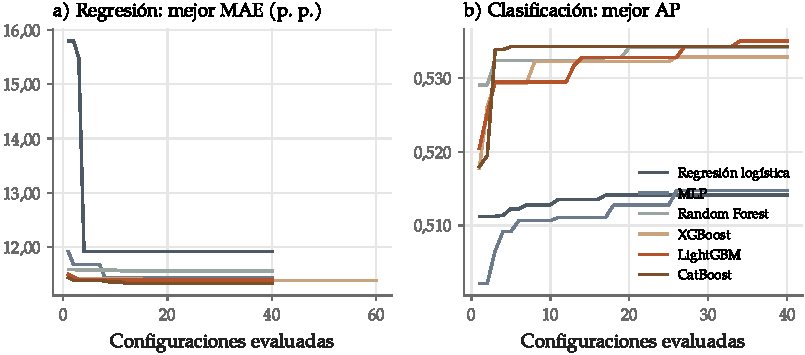
\includegraphics[width=.8\textwidth]{fig_busqueda}
\caption{Convergencia de la búsqueda aleatoria: mejor MAE promedio de validación (a) y mejor AP de validación (b) según el número de configuraciones evaluadas.}\label{fig:busqueda}
\end{figure}
\FloatBarrier

\footnotesize
\begin{longtable}{llrp{7.4cm}}
\caption{Hiperparámetros elegidos por búsqueda aleatoria (número de configuraciones evaluadas en la tercera columna). Las dos búsquedas de cada modelo usaron la misma semilla y, por tanto, la misma secuencia de configuraciones; en Random Forest, la misma configuración resultó la mejor en ambas tareas, por lo que sus valores coinciden.}\label{tab:hiper}\\
\toprule Tarea & Modelo & $N$ & Valores elegidos\\ \midrule\endfirsthead
\toprule Tarea & Modelo & $N$ & Valores elegidos\\ \midrule\endhead
\bottomrule\endfoot
Reg. & Regresión cuantílica & 40 & $\alpha$ $3{,}4\cdot10^{-7}$; penal. L1 \\
Reg. & MLP & 40 & $\alpha$ 0{,}0067; capas (128, 64); tasa 0{,}0019 \\
Reg. & Random Forest & 40 & hoja mín. 21; frac. var. 0{,}405; prof. 19 \\
Reg. & XGBoost & 60 & frac. col. 0{,}451; tasa 0{,}022; peso mín. 7{,}370; árboles 424; prof. 7; submuestra 0{,}751 \\
Reg. & LightGBM & 40 & frac. col. 0{,}636; hojas 33; $\lambda$ 0{,}0019; tasa 0{,}023; obs. hoja 135; árboles 581; submuestra 0{,}948 \\
Reg. & CatBoost & 40 & $\lambda$ 2{,}288; tasa 0{,}044; árboles 307; prof. 7 \\
\midrule
Clas. & Regresión logística & 40 & $C$ 0{,}0030; penal. L1 \\
Clas. & MLP & 40 & $\alpha$ $1{,}9\cdot10^{-5}$; capas (64); tasa $2{,}0\cdot10^{-4}$ \\
Clas. & Random Forest & 40 & hoja mín. 21; frac. var. 0{,}405; prof. 19 \\
Clas. & XGBoost & 40 & frac. col. 0{,}573; tasa 0{,}040; peso mín. 21{,}485; árboles 190; prof. 6; submuestra 0{,}637 \\
Clas. & LightGBM & 40 & frac. col. 0{,}722; hojas 89; $\lambda$ 9{,}149; tasa 0{,}029; obs. hoja 83; árboles 166; submuestra 0{,}705 \\
Clas. & CatBoost & 40 & $\lambda$ 4{,}448; tasa 0{,}039; árboles 447; prof. 4 \\
Cuant. & LightGBM & 40 & frac. col. 0{,}808; hojas 12; $\lambda$ 8{,}209; tasa 0{,}025; obs. hoja 106; árboles 611; submuestra 0{,}765 \\
\end{longtable}
\normalsize


\clearpage
\subsection*{Verificación de las implementaciones propias}

La regresión cuantílica por descenso de gradiente se comparó con la solución exacta en una submuestra; la red neuronal con pérdida absoluta, comparando su gradiente con diferencias finitas y comprobando en datos simulados que estima la mediana y no la media, y el Random Forest de LightGBM, con el de scikit-learn con los mismos hiperparámetros. Las tres coinciden con su referencia (tabla~\ref{tab:verificacion}). En la regresión cuantílica, la correlación entre los coeficientes (0,77) es menor que entre las predicciones (0,998), porque varias variables están muy correlacionadas entre sí y distintas combinaciones de coeficientes dan casi el mismo ajuste. El bosque de LightGBM tiene un error 0,19 puntos mayor que el de scikit-learn en la submuestra, con predicciones muy correlacionadas.

\begin{table}[htbp]\centering\footnotesize
\caption{Verificación de las implementaciones no estándar (submuestras de 6\,000 y 3\,000 filas de entrenamiento, 4\,000 de validación; simulación con ruido exponencial centrado en la mediana)}\label{tab:verificacion}
\begin{adjustbox}{max width=\textwidth}\begin{tabular}{llr}\toprule
Implementación & Comprobación & Resultado\\ \midrule
Regresión cuantílica & MAE (p.\,p.) solución exacta / descenso de gradiente & 11{,}58 / 11{,}59 \\
 & Correlación de predicciones / de coeficientes & 0{,}9979 / 0{,}769 \\
MLP (error absoluto) & Error relativo del gradiente, mediana / máximo & $1{,}8\cdot10^{-9}$ / $8{,}1\cdot10^{-6}$ \\
 & Simulación: distancia a la mediana / a la media (pérdida absoluta) & 0{,}059 / 0{,}334 \\
 & Simulación: distancia a la mediana / a la media (pérdida cuadrática) & 0{,}337 / 0{,}045 \\
Random Forest & MAE (p.\,p.) LightGBM / scikit-learn / paseo aleatorio & 11{,}81 / 11{,}62 / 13{,}43 \\
 & Correlación de predicciones & 0{,}954 \\
\bottomrule\end{tabular}\end{adjustbox}\end{table}





\section{Cobertura por central}
\label{ap:centrales}

\begin{table}[htbp]\centering\scriptsize
\caption{Cobertura por central: series en el panel, porcentaje de meses con precio desde que empieza cada serie, mediana del cambio mensual absoluto (p.~p.) y porcentaje de alzas mayores al 15\,\%}\label{tab:centrales}
\begin{adjustbox}{max width=\textwidth}\begin{tabular}{llrrrr}\toprule
Central & Ciudad & Series & Con precio (\%) & Cambio típico & Alzas (\%)\\ \midrule
Corabastos & Bogotá & 84 & 96{,}9 & 9{,}2 & 20{,}2 \\
Central Mayorista de Antioquia & Medellín & 80 & 97{,}3 & 8{,}5 & 18{,}5 \\
Centroabastos & Bucaramanga & 68 & 96{,}8 & 8{,}9 & 19{,}8 \\
CAV & Villavicencio & 65 & 96{,}1 & 8{,}5 & 18{,}6 \\
Surabastos & Neiva & 65 & 94{,}1 & 9{,}0 & 18{,}9 \\
Mercasa & Pereira & 63 & 95{,}8 & 7{,}2 & 16{,}9 \\
Mercar & Armenia & 63 & 93{,}3 & 7{,}8 & 15{,}9 \\
Cenabastos & Cúcuta & 62 & 96{,}2 & 8{,}1 & 17{,}3 \\
Santa Elena & Cali & 59 & 96{,}8 & 7{,}4 & 17{,}2 \\
Complejo de Servicios del Sur & Tunja & 59 & 95{,}4 & 11{,}0 & 22{,}5 \\
Centro Galerías & Manizales & 57 & 95{,}5 & 7{,}3 & 16{,}4 \\
Cavasa & Cali & 50 & 94{,}9 & 10{,}9 & 22{,}4 \\
Plaza Minorista José María Villa & Medellín & 49 & 95{,}1 & 10{,}4 & 21{,}1 \\
Plaza La 21 & Ibagué & 47 & 89{,}7 & 10{,}1 & 21{,}6 \\
Barranquillita & Barranquilla & 46 & 94{,}7 & 5{,}6 & 14{,}2 \\
Plaza de mercado del barrio Bolívar & Popayán & 43 & 92{,}2 & 6{,}6 & 15{,}1 \\
Nuevo Mercado & Sincelejo & 43 & 92{,}6 & 7{,}5 & 16{,}8 \\
Bazurto & Cartagena & 43 & 94{,}8 & 6{,}7 & 16{,}4 \\
Mercado del Sur & Montería & 43 & 94{,}3 & 6{,}7 & 14{,}7 \\
El Potrerillo & Pasto & 41 & 92{,}8 & 10{,}4 & 20{,}6 \\
Granabastos & Barranquilla & 33 & 93{,}2 & 5{,}2 & 13{,}2 \\
Mercabastos & Valledupar & 26 & 93{,}7 & 10{,}0 & 21{,}0 \\
Santa Marta (Magdalena) & Santa Marta & 24 & 87{,}8 & 8{,}8 & 17{,}9 \\
Mercado Nuevo & Valledupar & 20 & 82{,}5 & 5{,}7 & 14{,}2 \\
La Nueva Sexta & Cúcuta & 9 & 91{,}3 & 2{,}7 & 8{,}6 \\
Paloquemao & Bogotá & 9 & 78{,}4 & 2{,}4 & 1{,}6 \\
Centro de acopio & Ipiales & 6 & 76{,}0 & 16{,}6 & 27{,}8 \\
Plaza Las Flores & Bogotá & 3 & 89{,}8 & 2{,}3 & 1{,}7 \\
\bottomrule\end{tabular}\end{adjustbox}\end{table}


\imprimirbibliografia

\end{document}
